\documentclass[11pt,a4paper]{article}
\usepackage[margin=2cm]{geometry}
\usepackage{booktabs,xcolor,hyperref,enumitem,graphicx,float,caption,array}
\definecolor{good}{HTML}{2E7D4F}\definecolor{amber}{HTML}{B07D1A}\definecolor{bad}{HTML}{B5403A}
\setlist{itemsep=1pt,topsep=2pt}\emergencystretch=3em
\title{Issuer memos: one analyst, four groups of methods}
\author{FundamentalQuantmental HY Analyst: one memo per company, written by the process}
\date{Data as known on 2026-09-18}
\begin{document}
\maketitle
\noindent\fcolorbox{gray}{gray!6}{\parbox{\dimexpr\linewidth-2\fboxsep-2\fboxrule-1pt}{\sloppy
\textbf{How these memos are made.} One analyst runs every company through four groups of methods. Group 1 is the core process: Gatto's seven steps, our method, our rulebook and the relative value paper. Group 2 is the set of methods we built: the two clocks, the fair line and the pair, the economic stories, the gate and the health panel. Group 3 applies the lender's checklists (the credit skills) where public filings allow. Group 4 applies two books: Kricheff, and Ganguin and Bilardello (S\&P). Each group gives its own estimate of expected profit above a hedge, in bp a year. The combined estimate weighs five buckets as the user set them (core process 45.0\%, two clocks 20.0\%, built methods (rest) 11.7\%, credit skills 11.7\%, books 11.7\%) and pays trading costs once. Each step is \textcolor{good}{done}, \textcolor{amber}{partial} (it ran but needs an analyst input), or \textcolor{bad}{blocked}. Missing inputs appear as open questions.}}

\section*{All issuers, ranked by the combined view}
The combined column is after trading costs; the five bucket columns (with their weights) are before costs, in bp a year. ``Cases'' is the weighted cases and stories after costs. ``Best alt.'' is the position the same money would rather hold (cash when nothing in the run beats it). \textbf{Alpha sizes are uncalibrated}: in the backtest, realised alpha was about 0.08 times the predicted alpha, so ``Calibrated'' multiplies the combined number by that slope (decision page 2026-10-22-alpha-backtest-design). The slope is not significant, so the numbers rank the issuers but do not size positions.
\begin{center}\scriptsize\setlength{\tabcolsep}{2pt}\begin{tabular}{@{}rlrrrrrrrrll@{}}\toprule
Rank & Issuer & Combined & Calibrated & G1 (45\%) & G2 clocks (20\%) & G2 rest (12\%) & G3 (12\%) & G4 (12\%) & Cases & Best alt. & Gate \\\midrule
1 & CRWV & \textbf{-61} & -5 & +246 & -309 & +426 & -215 & +123 & +213 & NCLH & Watch \\
2 & THC & \textbf{-101} & -8 & +22 & +183 & +60 & +0 & +169 & -103 & NCLH & Pass \\
3 & CCL & \textbf{-110} & -9 & +72 & +88 & +16 & +0 & +100 & -116 & NCLH & Pass \\
4 & HCA & \textbf{-139} & -11 & +47 & +197 & -82 & +0 & -113 & -231 & NCLH & Pass \\
5 & NCLH & \textbf{-190} & -15 & -58 & +102 & +62 & -215 & +11 & -100 & CCL & Pass \\
6 & ORCL & \textbf{-201} & -16 & +92 & -158 & -88 & -215 & -16 & -173 & NCLH & Pass \\
7 & WYNN & \textbf{-205} & -16 & -22 & +4 & -58 & +0 & -148 & -336 & NCLH & Pass \\
8 & MGM & \textbf{-220} & -17 & -4 & -108 & -86 & +0 & -126 & -395 & NCLH & Pass \\
\bottomrule\end{tabular}\end{center}

\section*{What each part of a memo answers}
\begin{center}\footnotesize\begin{tabular}{@{}lp{7.2cm}p{6.4cm}@{}}\toprule Memo part & What it answers & Where it comes from \\\midrule
Top & The call and the combined view of the four groups & Methodology 8; F10, F12.1; decision 2026-10-22-four-group-combination \\
G1 & The business, earnings, cash, debt, value, the funding gap, the refinancing shock, the decision against cash & Gatto steps 1-7; M4.1-4.3, M6, M7.5; F2-F5, F7; RV PDF (hyrv mapping items 1-4; C2, C3) \\
G2 & The two clocks, the stories and cases, relative value and the pair, expected profit, the gate, the health panel & M4.7, M5.1-5.4, M7.4-7.5; F6, F8, F9, F10 S4 \\
G3 & Add-backs, the FCF check, covenant headroom, watchlist, trajectory, memo structure & hy-model-standards; ebitda-addback-treatment; covenant-compliance; borrower-monitoring; credit-memo-standards \\
G4 & Kricheff's cash bridge, ratio set, snapshot and spread per turn; the S\&P profiles and anchor & Kricheff ch. 9, 10, 21, 24; Ganguin and Bilardello ch. 2-5, 10, App. E \\
End & Coming events, open questions, the record & F11, F12 \\
\bottomrule\end{tabular}\end{center}

\section*{Which steps ran}
\textcolor{good}{\textbf{D}} done, \textcolor{amber}{\textbf{P}} partial (ran; needs an analyst input), \textcolor{bad}{\textbf{B}} blocked.
\begin{center}\footnotesize
\begin{tabular}{@{}lccccccccccccccccc@{}}\toprule
 & \rotatebox{90}{Load the data} & \rotatebox{90}{Describe the business} & \rotatebox{90}{Check the earnings} & \rotatebox{90}{Cash and debt due} & \rotatebox{90}{Debt, ratios, covenants} & \rotatebox{90}{Bills against contracts} & \rotatebox{90}{Economic stories} & \rotatebox{90}{Company value} & \rotatebox{90}{Compare with peers} & \rotatebox{90}{Compare the pair} & \rotatebox{90}{Expected profit} & \rotatebox{90}{Price against our view} & \rotatebox{90}{Events and watchlist} & \rotatebox{90}{Health check panel} & \rotatebox{90}{Combined view} & \rotatebox{90}{Size calibration} & \rotatebox{90}{Decision against cash} \\\midrule
CRWV & \textcolor{good}{\textbf{D}} & \textcolor{amber}{\textbf{P}} & \textcolor{amber}{\textbf{P}} & \textcolor{amber}{\textbf{P}} & \textcolor{amber}{\textbf{P}} & \textcolor{good}{\textbf{D}} & \textcolor{amber}{\textbf{P}} & \textcolor{amber}{\textbf{P}} & \textcolor{amber}{\textbf{P}} & \textcolor{good}{\textbf{D}} & \textcolor{amber}{\textbf{P}} & \textcolor{amber}{\textbf{P}} & \textcolor{amber}{\textbf{P}} & \textcolor{good}{\textbf{D}} & \textcolor{amber}{\textbf{P}} & \textcolor{amber}{\textbf{P}} & \textcolor{amber}{\textbf{P}} \\
ORCL & \textcolor{good}{\textbf{D}} & \textcolor{amber}{\textbf{P}} & \textcolor{amber}{\textbf{P}} & \textcolor{amber}{\textbf{P}} & \textcolor{amber}{\textbf{P}} & \textcolor{good}{\textbf{D}} & \textcolor{amber}{\textbf{P}} & \textcolor{amber}{\textbf{P}} & \textcolor{amber}{\textbf{P}} & \textcolor{good}{\textbf{D}} & \textcolor{amber}{\textbf{P}} & \textcolor{amber}{\textbf{P}} & \textcolor{amber}{\textbf{P}} & \textcolor{good}{\textbf{D}} & \textcolor{amber}{\textbf{P}} & \textcolor{amber}{\textbf{P}} & \textcolor{amber}{\textbf{P}} \\
HCA & \textcolor{good}{\textbf{D}} & \textcolor{amber}{\textbf{P}} & \textcolor{amber}{\textbf{P}} & \textcolor{amber}{\textbf{P}} & \textcolor{amber}{\textbf{P}} & \textcolor{good}{\textbf{D}} & \textcolor{amber}{\textbf{P}} & \textcolor{amber}{\textbf{P}} & \textcolor{amber}{\textbf{P}} & \textcolor{good}{\textbf{D}} & \textcolor{amber}{\textbf{P}} & \textcolor{amber}{\textbf{P}} & \textcolor{amber}{\textbf{P}} & \textcolor{good}{\textbf{D}} & \textcolor{amber}{\textbf{P}} & \textcolor{amber}{\textbf{P}} & \textcolor{amber}{\textbf{P}} \\
THC & \textcolor{good}{\textbf{D}} & \textcolor{amber}{\textbf{P}} & \textcolor{amber}{\textbf{P}} & \textcolor{amber}{\textbf{P}} & \textcolor{amber}{\textbf{P}} & \textcolor{good}{\textbf{D}} & \textcolor{amber}{\textbf{P}} & \textcolor{amber}{\textbf{P}} & \textcolor{amber}{\textbf{P}} & \textcolor{good}{\textbf{D}} & \textcolor{amber}{\textbf{P}} & \textcolor{amber}{\textbf{P}} & \textcolor{amber}{\textbf{P}} & \textcolor{good}{\textbf{D}} & \textcolor{amber}{\textbf{P}} & \textcolor{amber}{\textbf{P}} & \textcolor{amber}{\textbf{P}} \\
CCL & \textcolor{good}{\textbf{D}} & \textcolor{amber}{\textbf{P}} & \textcolor{amber}{\textbf{P}} & \textcolor{amber}{\textbf{P}} & \textcolor{amber}{\textbf{P}} & \textcolor{good}{\textbf{D}} & \textcolor{amber}{\textbf{P}} & \textcolor{amber}{\textbf{P}} & \textcolor{amber}{\textbf{P}} & \textcolor{good}{\textbf{D}} & \textcolor{amber}{\textbf{P}} & \textcolor{amber}{\textbf{P}} & \textcolor{amber}{\textbf{P}} & \textcolor{good}{\textbf{D}} & \textcolor{amber}{\textbf{P}} & \textcolor{amber}{\textbf{P}} & \textcolor{amber}{\textbf{P}} \\
NCLH & \textcolor{good}{\textbf{D}} & \textcolor{amber}{\textbf{P}} & \textcolor{amber}{\textbf{P}} & \textcolor{amber}{\textbf{P}} & \textcolor{amber}{\textbf{P}} & \textcolor{good}{\textbf{D}} & \textcolor{amber}{\textbf{P}} & \textcolor{amber}{\textbf{P}} & \textcolor{amber}{\textbf{P}} & \textcolor{good}{\textbf{D}} & \textcolor{amber}{\textbf{P}} & \textcolor{amber}{\textbf{P}} & \textcolor{amber}{\textbf{P}} & \textcolor{good}{\textbf{D}} & \textcolor{amber}{\textbf{P}} & \textcolor{amber}{\textbf{P}} & \textcolor{amber}{\textbf{P}} \\
MGM & \textcolor{good}{\textbf{D}} & \textcolor{amber}{\textbf{P}} & \textcolor{amber}{\textbf{P}} & \textcolor{amber}{\textbf{P}} & \textcolor{amber}{\textbf{P}} & \textcolor{good}{\textbf{D}} & \textcolor{amber}{\textbf{P}} & \textcolor{amber}{\textbf{P}} & \textcolor{amber}{\textbf{P}} & \textcolor{good}{\textbf{D}} & \textcolor{amber}{\textbf{P}} & \textcolor{amber}{\textbf{P}} & \textcolor{amber}{\textbf{P}} & \textcolor{good}{\textbf{D}} & \textcolor{amber}{\textbf{P}} & \textcolor{amber}{\textbf{P}} & \textcolor{amber}{\textbf{P}} \\
WYNN & \textcolor{good}{\textbf{D}} & \textcolor{amber}{\textbf{P}} & \textcolor{amber}{\textbf{P}} & \textcolor{amber}{\textbf{P}} & \textcolor{amber}{\textbf{P}} & \textcolor{good}{\textbf{D}} & \textcolor{amber}{\textbf{P}} & \textcolor{amber}{\textbf{P}} & \textcolor{amber}{\textbf{P}} & \textcolor{good}{\textbf{D}} & \textcolor{amber}{\textbf{P}} & \textcolor{amber}{\textbf{P}} & \textcolor{amber}{\textbf{P}} & \textcolor{good}{\textbf{D}} & \textcolor{amber}{\textbf{P}} & \textcolor{amber}{\textbf{P}} & \textcolor{amber}{\textbf{P}} \\
\bottomrule\end{tabular}\end{center}

\section*{The economic stories used in every memo}
Probabilities combine economists' forecasts (Philadelphia Fed survey, Fed projections, Treasury market) with the stage of the cycle (expansion).
\begin{center}\footnotesize\begin{tabular}{@{}lrrrr@{}}\toprule Story & Chance & GDP growth & Fed rate in 2 years & High yield spread (bp) \\\midrule
soft landing & 86\% & 2.5\% & 3.9\% & 142 \\
recession & 2\% & -0.0\% & 2.6\% & 369 \\
higher for longer & 8\% & 2.2\% & 5.5\% & 168 \\
disinflation rally & 4\% & 2.8\% & 2.1\% & 110 \\
stagflation & 0\% & -0.1\% & 4.4\% & 376 \\
\bottomrule\end{tabular}\end{center}
\newpage
\section*{Words used}
\begin{description}
\item[Spread] The extra yield a bond pays over a US Treasury of the same maturity. More risk, more spread.
\item[bp (basis point)] One hundredth of a percent. 100 bp = 1\%.
\item[EBITDA] Yearly earnings before interest, tax, depreciation and amortisation: the cash the business makes before paying lenders.
\item[EBITDAR] EBITDA before rent. Used when rent is one of the bills.
\item[Add-back] A cost the company takes out of its own earnings figure because it calls the cost a one-off.
\item[Leverage] Debt divided by yearly earnings. With leases: (debt + leases) / (EBITDA + rent). 3x means three years of earnings.
\item[Coverage] How many times earnings (after capital spending, where stated) pay the interest bill.
\item[Liquidity] Cash plus unused credit lines, less the cash the business needs to run.
\item[Funding gap] Liquidity plus free cash flow, less the debt that falls due, quarter by quarter, if no lender refinances. Below zero, the company needs new money.
\item[Refinancing shock] The extra yearly interest when debt that falls due is refinanced at today's rates and spread.
\item[Covenant headroom] How far earnings (or cash) can fall before a loan test is broken.
\item[Watchlist] The lender's list of borrowers to watch: watch closely, watchlist, or workout.
\item[Two clocks] One clock counts the bills (rent, debt, interest) the company owes each year; the other counts the revenue customers have signed for. When the bills outlast the contracts, bondholders bet on renewals.
\item[Fair spread] The spread a company with this leverage pays, read off a line fitted across the companies in the run.
\item[Economic story] One of five views of the next two years, each with a probability from economists' forecasts and the stage of the cycle.
\item[Breakeven default probability] The yearly default rate at which the spread only pays for the loss in default. Our default chance below it favours the bond.
\item[Loss on price] What a holder loses in default per unit paid for the bond: price less the recovery, with the recovery discounted for the wait.
\item[Expected profit (alpha)] What the bond should earn above a hedge, after expected default losses; in bp a year.
\item[Decision against cash] The same money in the bond or in cash for six months, across every story and the default case.
\item[Spread per turn] The spread divided by leverage: bp paid for each year of earnings the debt represents.
\item[S\&P risk score] A 1 (safest) to 10 (default) score that blends business risk and financial risk; it maps to a rating class.
\item[Open question] A number the data cannot give. An analyst must find it before the memo becomes a call.
\end{description}
\newpage
\section*{CoreWeave (CRWV)}\pdfbookmark[1]{CRWV}{bm-CRWV}\label{memo-start-CRWV}
\par\noindent\fcolorbox{gray}{gray!6}{\parbox{\dimexpr\linewidth-2\fboxsep-2\fboxrule-1pt}{\sloppy \textbf{Recommendation.} Watch. The bond looks cheap by more than the model's noise, every check points the same way, and the expected profit beats trading costs. Before it becomes a trade, an analyst must name a dated event that would close the gap and the level that would prove the view wrong. If the money went elsewhere, the best alternative in this run is NCLH. Position size and hedge: open until the call passes.}}

\subsection*{The combined view: four groups, one estimate}
Each group of methods estimates the same thing: what the bond should earn above a hedge, in bp a year. The combined estimate weighs the four groups. It ranks 1 of the issuers in this run. 3 of 5 groups point the same way as the combination.
\begin{center}\footnotesize\setlength{\tabcolsep}{3.5pt}\begin{tabular}{@{}lrrrl@{}}\toprule
Group & bp a year & Weight & Adds & Call \\\midrule
G1. Core process & +246 & 45\% & +111 & \textcolor{good}{supports owning} \\
G2 clocks. Two clocks & -309 & 20\% & -62 & \textcolor{bad}{against owning} \\
G2 rest. Built methods (rest) & +426 & 12\% & +50 & \textcolor{good}{supports owning} \\
G3. Credit skills & -215 & 12\% & -25 & \textcolor{bad}{against owning} \\
G4. Books & +123 & 12\% & +14 & \textcolor{amber}{leans to owning} \\
\textbf{Combined, before trading costs} &  &  & \textbf{+88} &  \\
Trading costs &  &  & -149 &  \\
\textbf{Combined, after trading costs} &  &  & \textbf{-61} &  \\
Weighted cases and stories alone, after costs &  &  & +213 &  \\
Calibrated: after-cost number x measured slope 0.079 &  &  & -5 &  \\
\bottomrule\end{tabular}\end{center}
Against the weighted cases and stories alone, the combination is 275 bp a year lower: the other methods take away from the case for owning the bond. A group that supports owning must beat the trading costs on its own. The weights are the user's choice: core process 45\%, two clocks 20\%, and 11.7\% each for the rest of the built methods, the credit skills and the books. The backtest alone would have put most weight on the built methods.
\par\noindent\fcolorbox{gray}{gray!6}{\parbox{\dimexpr\linewidth-2\fboxsep-2\fboxrule-1pt}{\sloppy \textbf{Alpha sizes are uncalibrated.} The backtest (2008 to 2026) shows that this kind of estimate ranks bonds well but overstates the size of the move. Realised alpha has been about 0.08 times the predicted alpha (standard error 0.05; 0.25 since 2019). The calibrated number multiplies by that slope: -5 bp a year after costs (-15 on the 2019 slope). The slope is not above zero by two standard errors, so the number ranks the bond but does not size it. Decision page: 2026-10-22-alpha-backtest-design. The backtest has no default-loss term yet.}}

\section*{G1. Core process: Gatto's steps, our method and rulebook, the relative value paper}
\par\noindent\fcolorbox{gray}{gray!6}{\parbox{\dimexpr\linewidth-2\fboxsep-2\fboxrule-1pt}{\sloppy \textbf{Verdict: \textcolor{good}{supports owning}.} This group reads Gatto's seven steps, our method and rulebook, and the relative value paper. Its estimate of expected profit is +246 bp a year before trading costs (costs are 149 bp a year); 2 of 4 of its weighted estimates point the same way. It carries 45\% of the combined view and ranks 1 of the issuers on this group alone. Best alternative for the same money: NCLH.}}
\begin{center}\footnotesize\setlength{\tabcolsep}{3.5pt}\begin{tabular}{@{}p{6.2cm}rrrp{4.2cm}@{}}\toprule
Estimate & bp a year & Weight in group & Adds & Where it comes from \\\midrule
Default chance the price assumes (shown, weight 0) & +120 & 0\% & +0 & F9; mapping C2 \\
Earnings quality, add-backs, FCF check (can only lower) & +0 & 25\% & +0 & F3; ebitda-addback-treatment; hy-model-standards \\
Access to new money and the funding gap & -326 & 25\% & -82 & F4; RV PDF E75-E76 \\
Debt against market value & +23 & 25\% & +6 & F7.7 \\
Return above cash, repriced in every story & +1,289 & 25\% & +322 & RV PDF E50-E60; C1, C3 \\
\bottomrule\end{tabular}\end{center}
\subsection*{G1.1 Thesis}
The bond pays 739 bp over Treasuries at 5 years. A company with its leverage (8.9x with leases) pays 574 bp on the fair line, so the bond is cheap by 165 bp. The bills outlast the signed contracts (section G2.1), so part of the extra spread pays for a renewal bet that the line does not see. What would reveal it, and when: open question.
\subsection*{G1.2 The business}
\begin{enumerate}
\item \textbf{What it sells:} CoreWeave is The Essential Cloud for AITM, purpose-built to accelerate breakthroughs by AI pioneers, from leading research labs to enterprises fueling business growth. Our CoreWeave Cloud platform enables the full lifecycle of AI, including large-scale model training, inference, data movement, continuous iteration, and agentic workflows.
\item \textbf{How it earns:} revenue 7.6bn a year at a 50\% EBITDA margin.
\item \textbf{What it must spend to stand still:} rent of about \$2.1bn a year, plus maintenance capital spending.
\item \textbf{Competition:} open question.
\item \textbf{What breaks it:} contracts roll off or churn; the asset value cycle turns; the largest customer is 36\% of revenue.
\end{enumerate}
Business type: A5; flags: M3 concentration.
\subsection*{G1.3 Earnings, normalised}
Last 12 months: EBITDA \$3.8bn at a 50\% margin; margin trend over 8 quarters -1.6 (t-statistic: above 1 rising, below $-1$ falling). One-off items \$-0.0bn. Free cash flow \$-13.7bn: -363\% of EBITDA. Earnings-quality flags raised: EQ7 conversion, FCF check (waterfall against OCF less capex) (of 4 tests the data supports). The add-back detail is in section G3.1.
\subsection*{G1.4 Cash, the funding gap, and the refinancing shock}
\begin{center}\footnotesize\setlength{\tabcolsep}{3.5pt}\begin{tabular}{@{}lr@{}}\toprule
Item & Value \\\midrule
Cash & \$7.0bn \\
Unused credit lines (tagged) & \$0.0bn \\
Less cash needed to run & \$0.1bn \\
Liquidity & \$7.0bn \\
Runway at today's cash burn, all capital spending (quarters) & 2.0 \\
First quarter cash runs out, severe case, maintenance spending only & no shortfall in 8 quarters \\
First quarter cash runs out, severe case, all committed spending & 2 \\
\textbf{Runway we quote (the shortest)} & \textbf{2.0} (severe, committed capex) \\
Debt due in the next 18 months & \$10.6bn \\
Cash to meet debt due in a year, base case & 1.29x \\
Refinancing access score, likely story (0 to 6) & 3 \\
\bottomrule\end{tabular}\end{center}
\textbf{Funding gap if no lender refinances.} We add cash, the unused lines and the free cash flow of the cases, then take off the debt as it falls due, quarter by quarter. The minimum cash kept back is one month of cash operating costs (\$0.4bn).
\begin{center}\footnotesize\setlength{\tabcolsep}{3.5pt}\begin{tabular}{@{}lr@{}}\toprule
Measure & Value \\\midrule
Lowest point, likely story (maintenance spending only) & \$-5.4bn \\
First quarter below zero, likely story & quarter 6 \\
Lowest point with all capital spending & \$-45.4bn \\
First quarter below zero with all capital spending & quarter 2 \\
Lowest point, severe case & \$-9.0bn \\
Severe case with all capital spending: first quarter below zero & quarter 2 \\
Lowest point, weighted over the stories & \$-5.4bn \\
Debt due inside 8 quarters, share of all debt & 30\% \\
\bottomrule\end{tabular}\end{center}
\textbf{Refinancing shock.} \$10.6bn falls due in the next two years. It pays about 3.97\% today (derived cash interest rate (LTM interest / debt)). Refinanced at the forecast Treasury rate plus today's spread, yearly interest changes by \$0.9bn (23.8\% of EBITDA). Interest cover after refinancing: 1.7x; after capital spending -7.6x. Free cash flow after the shock: -40.9\% of debt.
\subsection*{G1.5 Debt: going-concern view}
\begin{center}\footnotesize\setlength{\tabcolsep}{3.5pt}\begin{tabular}{@{}lr@{}}\toprule
Measure & Value \\\midrule
Debt & \$35.6bn \\
Lease liabilities & \$16.5bn \\
EBITDA, last 12 months & \$3.8bn \\
Debt / EBITDA & 9.4x \\
(Debt + leases) / (EBITDA + rent) & 8.9x \\
Net debt / EBITDA & 8.0x \\
Coverage (after all capital spending) & -12.8x \\
Fixed-charge cover (after maintenance spending) & 0.54x \\
\bottomrule\end{tabular}\end{center}
\begin{center}\footnotesize\setlength{\tabcolsep}{3.5pt}\begin{tabular}{@{}lrrrrr@{}}\toprule
Bond & Coupon & Matures & Price & Yield & Spread (bp) \\\midrule
21873SAB4 & 9.25\% & 2030-06-01 & 93.7 & 11.37\% & 661 \\
21873SAC2 & 9.00\% & 2031-02-01 & 90.3 & 11.91\% & 714 \\
21873SAG3 & 9.75\% & 2031-10-01 & 89.8 & 12.54\% & 776 \\
21873SAK4 & 9.63\% & 2032-07-15 & 88.8 & 12.36\% & 755 \\
\bottomrule\end{tabular}\end{center}
Claims view (who is paid what in a default): open question until the debt documents are read.
\subsection*{G1.6 Company value}
Market value of the whole company \$85bn (shares \$55bn plus net debt): 22.6x EBITDA; debt is 42\% of it. Our own valuation range and the bonds' recovery if the company defaults: open questions (they need a peer set and a distressed multiple).
\subsection*{G1.7 The decision against cash}
We put the same money in the bond nearest five years (21873SAG3, 9.75\% due 2031-10-01, price 89.79 plus 4.51 accrued) or in six-month Treasury bills at 4.20\%. In each story the bond either survives and is repriced, or defaults and returns 35 per 100 (a 40\% recovery paid a year later, valued at 15\% a year). In default the holder loses 63\% of the price paid.
\begin{center}\footnotesize\setlength{\tabcolsep}{3.5pt}\begin{tabular}{@{}lr@{}}\toprule
Measure & Value \\\midrule
Expected return above cash, bp a year & +1,289 \\
Chance of a loss over six months & 4.0\% \\
Chance of doing worse than cash & 4.0\% \\
Average loss in the worst 5\% of outcomes & 30.6\% \\
Same, with rates and the market hedged out, bp a year & +613 \\
Best alternative in this run (worst 5\% loss within the 25\% budget) & NCLH \\
Return given up against that alternative, bp a year & -842 \\
\bottomrule\end{tabular}\end{center}
\section*{G2. Built methods: two clocks, stories and cases, relative value, the gate}
\par\noindent\fcolorbox{gray}{gray!6}{\parbox{\dimexpr\linewidth-2\fboxsep-2\fboxrule-1pt}{\sloppy \textbf{Verdict: \textcolor{good}{supports owning}.} This group reads the spread level, the fair line and the pair, the economic stories, the health panel. Its estimate of expected profit is +426 bp a year before trading costs (costs are 149 bp a year); 4 of 5 of its weighted estimates point the same way. It carries 12\% of the combined view and ranks 1 of the issuers on this group alone. Gate: watch.}}
\begin{center}\footnotesize\setlength{\tabcolsep}{3.5pt}\begin{tabular}{@{}p{6.2cm}rrrp{4.2cm}@{}}\toprule
Estimate & bp a year & Weight in group & Adds & Where it comes from \\\midrule
Spread level: the extra pay over the market (carry) & +571 & 42\% & +238 & Spec S14 E0; K15 \\
Weighted cases and stories & +363 & 25\% & +91 & M5.4, M7.5 \\
Spread against the fair line & +342 & 17\% & +57 & M7.4, M7.5 \\
The pair & +776 & 8\% & +65 & M7.4; F10 S4 \\
Health panel & -295 & 8\% & -25 & F8 \\
\bottomrule\end{tabular}\end{center}
\subsection*{G2.1 The two clocks: bills against what pays for them}
\par\noindent\fcolorbox{gray}{gray!6}{\parbox{\dimexpr\linewidth-2\fboxsep-2\fboxrule-1pt}{\sloppy \textbf{Verdict: \textcolor{bad}{against owning}.} This group reads the bills the company owes against the revenue customers have signed for. Its estimate of expected profit is -309 bp a year before trading costs (costs are 149 bp a year); 1 of 1 of its weighted estimates point the same way. It carries 20\% of the combined view and ranks 8 of the issuers on this group alone. The clocks count as their own bucket in the combined view.}}
\begin{center}\footnotesize\setlength{\tabcolsep}{3.5pt}\begin{tabular}{@{}p{6.2cm}rrrp{4.2cm}@{}}\toprule
Estimate & bp a year & Weight in group & Adds & Where it comes from \\\midrule
The two clocks & -309 & 100\% & -309 & M4.7 \\
\bottomrule\end{tabular}\end{center}
Fixed bills total \$106.4bn, centred 5.5 years out: leases in force \$29.4bn, signed leases not yet started \$35.5bn, debt principal \$35.6bn, interest \$4.7bn, purchase commitments \$1.2bn. That is 18.2 years of today's EBITDAR; next year's bills take 206\% of it.
\begin{center}\footnotesize\setlength{\tabcolsep}{3.5pt}\begin{tabular}{@{}lr@{}}\toprule
Measure & Value \\\midrule
Signed contracts (RPO) & \$103.7bn \\
Where bills centre / where contract cash centres & year 5.5 / year 2.6 \\
Contracts 99\% booked by & year 7 \\
Margin needed for contracts to pay every bill & over 100\% (no margin is enough) \\
Company margin (EBITDAR) & 77\% \\
Share of bills paid by contracts at that margin & 75\% \\
Bills due after the contracts end & \$32.6bn (31\%) \\
\quad of which debt to refinance & \$0.0bn (0\%) \\
\quad of which rent and purchases to recontract & \$32.6bn (31\%) \\
Revenue to sign after the contracts end & 4.1 years of today's revenue \\
Largest running shortfall & \$26.7bn \\
Top three customers & 72\% \\
Top customer stops paying & contracts pay 48\%; shortfall \$55.4bn \\
With excluded lease & contracts pay 66\%; shortfall \$41.4bn \\
Share paid by contracts at a 0.20 margin & 20\% \\
Share paid by contracts at a 0.35 margin & 34\% \\
Share paid by contracts at a 0.50 margin & 49\% \\
Share paid by contracts at a 0.77 margin & 75\% \\
\bottomrule\end{tabular}\end{center}
\subsection*{G2.2 Economic stories and cases}
Cases on the most likely story (soft landing), stage of the cycle: expansion.
\begin{center}\scriptsize\setlength{\tabcolsep}{3.5pt}\begin{tabular}{@{}lrrrrrrr@{}}\toprule
Case & Weight & Growth / qtr & Leverage in 1 yr & Peak leverage & Lowest liquidity & Cash runs out & Refi fails \\\midrule
base & 64\% & 8.0\% & 5.6x & 8.0x & \$5.6bn & no & no \\
down moderate & 11\% & 8.4\% & 6.6x & 8.6x & \$4.7bn & no & no \\
down severe & 4\% & 8.3\% & 9.3x & 9.3x & \$2.0bn & no & no \\
upside & 21\% & 8.3\% & 4.9x & 7.4x & \$6.5bn & no & no \\
\bottomrule\end{tabular}\end{center}
\begin{center}\scriptsize\setlength{\tabcolsep}{3.5pt}\begin{tabular}{@{}lrrrrrr@{}}\toprule
Story & Chance & Leverage in 1 yr & Peak leverage (down) & Refi fails & Default chance & Expected profit (bp/yr) \\\midrule
soft landing & 86\% & 5.7x & 9.3x & 0\% & 4.0\% & 348 \\
recession & 2\% & 6.0x & 9.9x & 100\% & 10.0\% & 919 \\
higher for longer & 8\% & 5.8x & 9.3x & 0\% & 4.7\% & 414 \\
disinflation rally & 4\% & 5.7x & 9.3x & 0\% & 3.1\% & 270 \\
stagflation & 0\% & 6.1x & 9.9x & 100\% & 10.2\% & 935 \\
\bottomrule\end{tabular}\end{center}
\subsection*{G2.3 Relative value and the pair}
Fair line: log spread = -5.64 + 0.312 x leverage, fitted on 8 issuers in this run. 5-year spread 739 bp against a fair 574 bp.
\textbf{Against peers.} Peers are the high yield bonds that traded in 2026-08-31 (733 bonds with leverage on file), in the same 3 to 7 year maturity bucket. Sector: Information Technology. Rating class: CCC (implied by leverage). A positive value means the issuer pays more than the median peer.
\begin{center}\footnotesize\setlength{\tabcolsep}{3.5pt}\begin{tabular}{@{}lrr@{}}\toprule
Peer group & Excess spread to peers (ESP) & Spread per turn against peers (E13) \\\midrule
Sector and rating & +78\% & +276\% \\
Sector only & +447\% & +103\% \\
Rating only & +169\% & +227\% \\
\bottomrule\end{tabular}\end{center}
\textbf{SPiDER}: No SPiDER: fewer than 6 annual EBITDA figures, a financial issuer, or non-positive sustainable EBITDA.
\textbf{Against ORCL.} Spreads at 5 years: CRWV 739 bp, ORCL 136 bp.
\begin{center}\footnotesize\setlength{\tabcolsep}{3.5pt}\begin{tabular}{@{}lrrr@{}}\toprule
Spread per & CRWV & ORCL & Cheaper \\\midrule
turn of leverage & 83 & 32 & CRWV \\
year of EBITDA that depends on renewal & 85 & 23 & CRWV \\
unit of breakeven margin & 721 & 165 & CRWV \\
year of clock gap & 257 & 28 & CRWV \\
\bottomrule\end{tabular}\end{center}
The fair line favours long CRWV, short ORCL: a gap of 159 bp, which halves in about 17 weeks on six months of trades. Under the stories the pair earns soft landing +348, recession +918, higher for longer +414, disinflation rally +270, stagflation +935 bp a year; weighted +363 bp before costs.
\subsection*{G2.4 Expected profit and price against our view}
Hedged 5-year bond over six months: 363 bp a year before trading costs, 213 bp after. It beats costs. The expected default loss is charged on the price paid: 63\% of it in default, not 60\% of face.
\begin{center}\footnotesize\setlength{\tabcolsep}{3.5pt}\begin{tabular}{@{}p{5.2cm}rrrrl@{}}\toprule
Question & Price assumes & Our view & Gap & Noise & Gap bigger than noise? \\\midrule
Default chance at the v0 price of risk (shown, not tested) & 6.0\% & 4.1\% & -1.9\% & open & not tested \\
Breakeven default probability, 12 months (loss on price) & 11.7\% & 4.1\% & -7.6\% & 5.9\% & yes \\
Leverage the spread is pricing & 9.75 & 8.94 & -0.81 & 0.90 & no \\
Spread against fair (bp) & 739 & 574 & -165 & 160 & yes \\
Rating class & open & BB & open & open & not tested \\
Recovery if default (per 1 of face, discounted for delay) & open & 0.35 & open & open & not tested \\
\bottomrule\end{tabular}\end{center}
The first row turns the spread into a default chance with a fixed price of risk. That is not a real default chance, so it is shown but not tested. The breakeven row asks a cleaner question: is our default chance below the rate at which the spread only just pays for default losses?
\subsection*{G2.5 Risks and the health panel}
\begin{itemize}\item Earnings after capital spending do not cover interest. Tracked by: coverage (-12.79). Resolves when: capital spending falls, or earnings rise.\item Earnings do not cover interest plus rent. Tracked by: fixed-charge cover (0.54). Resolves when: earnings rise or rent falls.\item Little of the earnings turns into free cash. Tracked by: cash conversion (fcf / ebitda) (-3.63). Resolves when: growth spending ends.\item Free cash flow repays little debt. Tracked by: free cash flow / debt (-0.38). Resolves when: free cash flow turns positive.\item Margins are falling. Tracked by: margin trend (t-statistic) (-1.61). Resolves when: two quarters of stable margins.\end{itemize}
\begin{center}\footnotesize\setlength{\tabcolsep}{3.5pt}\begin{tabular}{@{}lrl@{}}\toprule
Measure & Value & Band \\\midrule
Coverage & -12.79 & \textcolor{bad}{red} \\
Fixed-charge cover & 0.54 & \textcolor{bad}{red} \\
Cash conversion (FCF / EBITDA) & -3.63 & \textcolor{bad}{red} \\
Free cash flow / debt & -0.38 & \textcolor{bad}{red} \\
Margin trend (t-statistic) & -1.61 & \textcolor{bad}{red} \\
Cash to meet debt due in 1 year (base case) & 1.29 & \textcolor{amber}{amber} \\
Refinancing access score (0 to 6) & 3.00 & \textcolor{amber}{amber} \\
Earnings-quality flags & 2.00 & \textcolor{amber}{amber} \\
Weight on the downside cases & 0.15 & \textcolor{good}{green} \\
Chance debt due in 1 year is not covered & 0.04 & \textcolor{good}{green} \\
Chance cash runs out within 2 years & 0.00 & \textcolor{good}{green} \\
\bottomrule\end{tabular}\end{center}
\section*{G3. Credit skills: the lender's checklists applied to a public bond}
\par\noindent\fcolorbox{gray}{gray!6}{\parbox{\dimexpr\linewidth-2\fboxsep-2\fboxrule-1pt}{\sloppy \textbf{Verdict: \textcolor{bad}{against owning}.} This group reads the lender's checklists: add-backs, covenants, watchlist, trend, memo structure. Its estimate of expected profit is -215 bp a year before trading costs (costs are 149 bp a year); 1 of 1 of its weighted estimates point the same way. It carries 12\% of the combined view and ranks 6 of the issuers on this group alone. Its estimates can only lower the combined number: a clean checklist earns no credit. Watchlist: watchlist.}}
\begin{center}\footnotesize\setlength{\tabcolsep}{3.5pt}\begin{tabular}{@{}p{6.2cm}rrrp{4.2cm}@{}}\toprule
Estimate & bp a year & Weight in group & Adds & Where it comes from \\\midrule
Watchlist tier (can only lower) & -215 & 100\% & -215 & borrower-monitoring; covenant-compliance \\
\bottomrule\end{tabular}\end{center}
\subsection*{G3.1 Add-backs and their cash effect}
Reported EBITDA over the last 12 months is \$3.7bn. The company's own measure adds back \$0.0bn of one-off items to reach \$3.8bn: 0.5\% of reported EBITDA (a negative figure is a one-off gain taken out). This is under the 5\% line for one item. They do not recur in three quarters running. If every add-back were paid in cash, free cash flow would be \$-13.7bn. The two roads to free cash flow (the EBITDA bridge, \$-16.3bn; operating cash flow less capital spending, \$-13.7bn) differ by 71\% of EBITDA: above the 10\% tolerance, so an earnings-quality flag is raised. The add-back table by category is an open question: the data has one total line.
\subsection*{G3.2 Covenant headroom}
The 10-Q and 10-K text state no maintenance test level. Public bonds are often tested only when the company borrows more or pays out cash. Headroom is an open question until the credit agreement is read.
\subsection*{G3.3 Watchlist and trajectory}
Watchlist tier: \textbf{watchlist} because free cash flow is negative. EBITDA against the same months a year earlier: 100.8\% (no plan is public, so last year stands in for it). Open: liquidity against debt due cannot be read: revolver capacity not tagged.
\begin{center}\footnotesize\setlength{\tabcolsep}{3.5pt}\begin{tabular}{@{}llll@{}}\toprule
Measure & Direction & How much weight & Change on a year earlier, last quarter \\\midrule
revenue & improving & trend & 112.3\% \\
EBITDA & improving & trend & 121.2\% \\
EBITDA margin & improving & data point & 4.2\% \\
cash conversion & open & no data & n/a \\
\bottomrule\end{tabular}\end{center}
One quarter is an observation, two a data point, three or four a trend.
\subsection*{G3.4 Memo structure check}
\begin{center}\footnotesize\setlength{\tabcolsep}{3.5pt}\begin{tabular}{@{}lp{9cm}l@{}}\toprule
Section & Requires & Status \\\midrule
Executive summary & the business in one sentence, the opportunity, 2 to 3 reasons, 2 to 3 risks & \textcolor{good}{pass} \\
Capital structure & each tranche with face, coupon, maturity; senior, total and net leverage; LTV & \textcolor{amber}{open} \\
Terms & maintenance covenant levels and test dates; incurrence baskets; call terms & \textcolor{amber}{open} \\
Investment merits & free cash flow generation and the base-case deleveraging path & \textcolor{good}{pass} \\
Key risks & 3 to 5 issuer-specific risks, each with a mitigant & \textcolor{good}{pass} \\
Historical financials & at least 3 years, quarterly where available & \textcolor{amber}{open} \\
EBITDA adjustments & reported-to-adjusted bridge with the load as a share of EBITDA and the 5\% flag & \textcolor{amber}{open} \\
Model output & base and downside: EBITDA, FCF, leverage path, covenant headroom, liquidity runway & \textcolor{amber}{open} \\
\bottomrule\end{tabular}\end{center}
\textbf{Rules that do not transfer to a public bond:}\begin{itemize}\item The compliance certificate is the source of truth; public bonds have none. Headroom here uses our own ratio against a level parsed from the filing text. (covenant-compliance)\item Equity cures, step-down schedules and window-dressing checks need the credit agreement and monthly revolver balances. (covenant-compliance)\item Performance against the sponsor plan: no plan is public. The proxy is the same quarters a year earlier. (borrower-monitoring)\item Add-back caps and the certificate reconciliation live in the credit agreement. Compustat gives one special-items line, not the category table. (ebitda-addback-treatment)\item Sources and uses at entry, the sponsor case and the management call apply to new loans, not to bonds bought in the secondary market. (credit-memo-standards)\item Monthly lender packages do not exist for public issuers; XBRL quarters replace them. (quarterly-package-extraction)\end{itemize}
\section*{G4. Books: Kricheff, and Ganguin and Bilardello (S\&P)}
\par\noindent\fcolorbox{gray}{gray!6}{\parbox{\dimexpr\linewidth-2\fboxsep-2\fboxrule-1pt}{\sloppy \textbf{Verdict: \textcolor{amber}{leans to owning}.} This group reads Kricheff's cash bridge and ratios; the S\&P risk profiles and rating anchor. Its estimate of expected profit is +123 bp a year before trading costs (costs are 149 bp a year); 1 of 2 of its weighted estimates point the same way. It carries 12\% of the combined view and ranks 2 of the issuers on this group alone. S\&P anchor class: BB.}}
\begin{center}\footnotesize\setlength{\tabcolsep}{3.5pt}\begin{tabular}{@{}p{6.2cm}rrrp{4.2cm}@{}}\toprule
Estimate & bp a year & Weight in group & Adds & Where it comes from \\\midrule
Spread against the S\&P risk score & +246 & 50\% & +123 & Ganguin and Bilardello ch. 10 \\
Spread per turn of leverage (with the trap guard) & +0 & 50\% & +0 & Kricheff ch. 21 \\
\bottomrule\end{tabular}\end{center}
\subsection*{G4.1 Kricheff's cash-flow bridge and ratio set}
\begin{center}\footnotesize\setlength{\tabcolsep}{3.5pt}\begin{tabular}{@{}lr@{}}\toprule
Line (last 12 months) & Value \\\midrule
Adjusted EBITDA & \$3.8bn \\
less capital spending & \$20.6bn \\
less cash interest & \$1.3bn \\
less cash taxes & \$0.0bn \\
less increase in working capital & \$-1.8bn \\
\textbf{Free cash flow} & \textbf{\$-16.3bn} \\
Check: free cash flow before capital spending less operating cash flow & \$-2.7bn \\
Free cash flow after dividends & open (dividends not loaded) \\
\bottomrule\end{tabular}\end{center}
\begin{center}\footnotesize\setlength{\tabcolsep}{3.5pt}\begin{tabular}{@{}lrlr@{}}\toprule
Ratio & Value & Ratio & Value \\\midrule
EBITDA / cash interest & 2.9x & Debt / EBITDA & 9.4x \\
(EBITDA $-$ capex) / interest & -12.8x & Net debt / EBITDA & 7.6x \\
(EBITDA $-$ maintenance capex) / interest & -0.2x & Free cash flow / debt & -38.0\% \\
EBITDA / debt (highest rate at 1x cover) & 11.0\% & Market value / EBITDA & 22.2x \\
Equity cushion (1 $-$ debt / market value) & 57\% & Spread per turn of leverage & 78 bp \\
\bottomrule\end{tabular}\end{center}
Kricheff's snapshot rule: operating cash flow does not cover capital spending, so the issuer lives on the capital markets and needs the detailed liquidity work of section G1.4. Spread per turn compares the bond with the run's median of 38 bp a turn. Kricheff warns that a high spread per turn can mean weak cash flow, not value; read it with free cash flow / debt. The book measures leverage through each bond's rank; with no face by rank, total leverage stands in.
\subsection*{G4.2 The S\&P risk profiles and the rating anchor}
S\&P adds leases to debt and scores each ratio against the median of each rating class (CreditStats 2002, from the book). Scores run from 1 (safest) to 10 (default).
\begin{center}\footnotesize\setlength{\tabcolsep}{3.5pt}\begin{tabular}{@{}lrrrr@{}}\toprule
Ratio & Value & Score & BB median & B median \\\midrule
Debt / (debt + market value of equity) & 49\% & 5.9 & 57.5\% & 78.5\% \\
Funds from operations / debt & 10\% & 9.6 & 19.5\% & 10.8\% \\
Free operating cash flow / debt & -26\% & 10.0 & 8.5\% & 2.5\% \\
EBITDA / interest (with lease interest) & 1.8x & 9.5 & 3.2x & 1.8x \\
EBITDA margin & 50\% & 3.0 &  &  \\
\bottomrule\end{tabular}\end{center}
Financial risk score 8.1. Business risk score 5.8: industry 5, steadiness of sales 5 (year-on-year growth varies by 11.2\%), customer spread 8. The book puts 45\% of the weight on business risk for this class, so the default risk score is 7.0: the \textbf{BB} class. The line from score to spread across the run did not slope upward, so it gives no estimate. The 2005 edition has no modern anchor table; its own weighting table stands in for it.
\section*{Coming events, open questions, and the record}
\begin{itemize}\item Next quarterly results (estimated from filing cadence): 2026-11-11 (estimate).\item Debt due by 0.5 years out:  - \$4.4bn.\end{itemize}
\textbf{Open questions, most important first:}\begin{enumerate}\item A dated catalyst that would close the gap (G2).\item The observable and level that would prove the call wrong (G8).\item Face amount of each tranche and the secured debt ahead of the bonds (debt note table).\item Claims view: allowed claims by class and the entity map (framework F5).\item Maintenance covenant levels: none stated in the 10-Q or 10-K text; read the credit agreement exhibit (public bonds are often incurrence-only).\item The funding gap opens only because no revolver capacity is tagged: read the credit facility note before using the gap.\item Revolver commitment, draw, and borrowing base: not tagged; read the credit agreement note.\item F4 points 3 (unencumbered assets) and 6 (sponsor support) are scored 0 until read.\item Recovery, delay and the required return on a defaulted claim are v0 (R = 0.4, tau = 1 year, k = 15\%); the claims view and documents replace them.\item Peer set of at least four issuers of the same archetype (F3.3) for the valuation range (F7.1).\end{enumerate}
\textbf{Record (filled at exit):} exit date; return against the rating-matched index; worst point against the index; reason; the rule that would have helped.
\newpage
\begin{figure}[H]\centering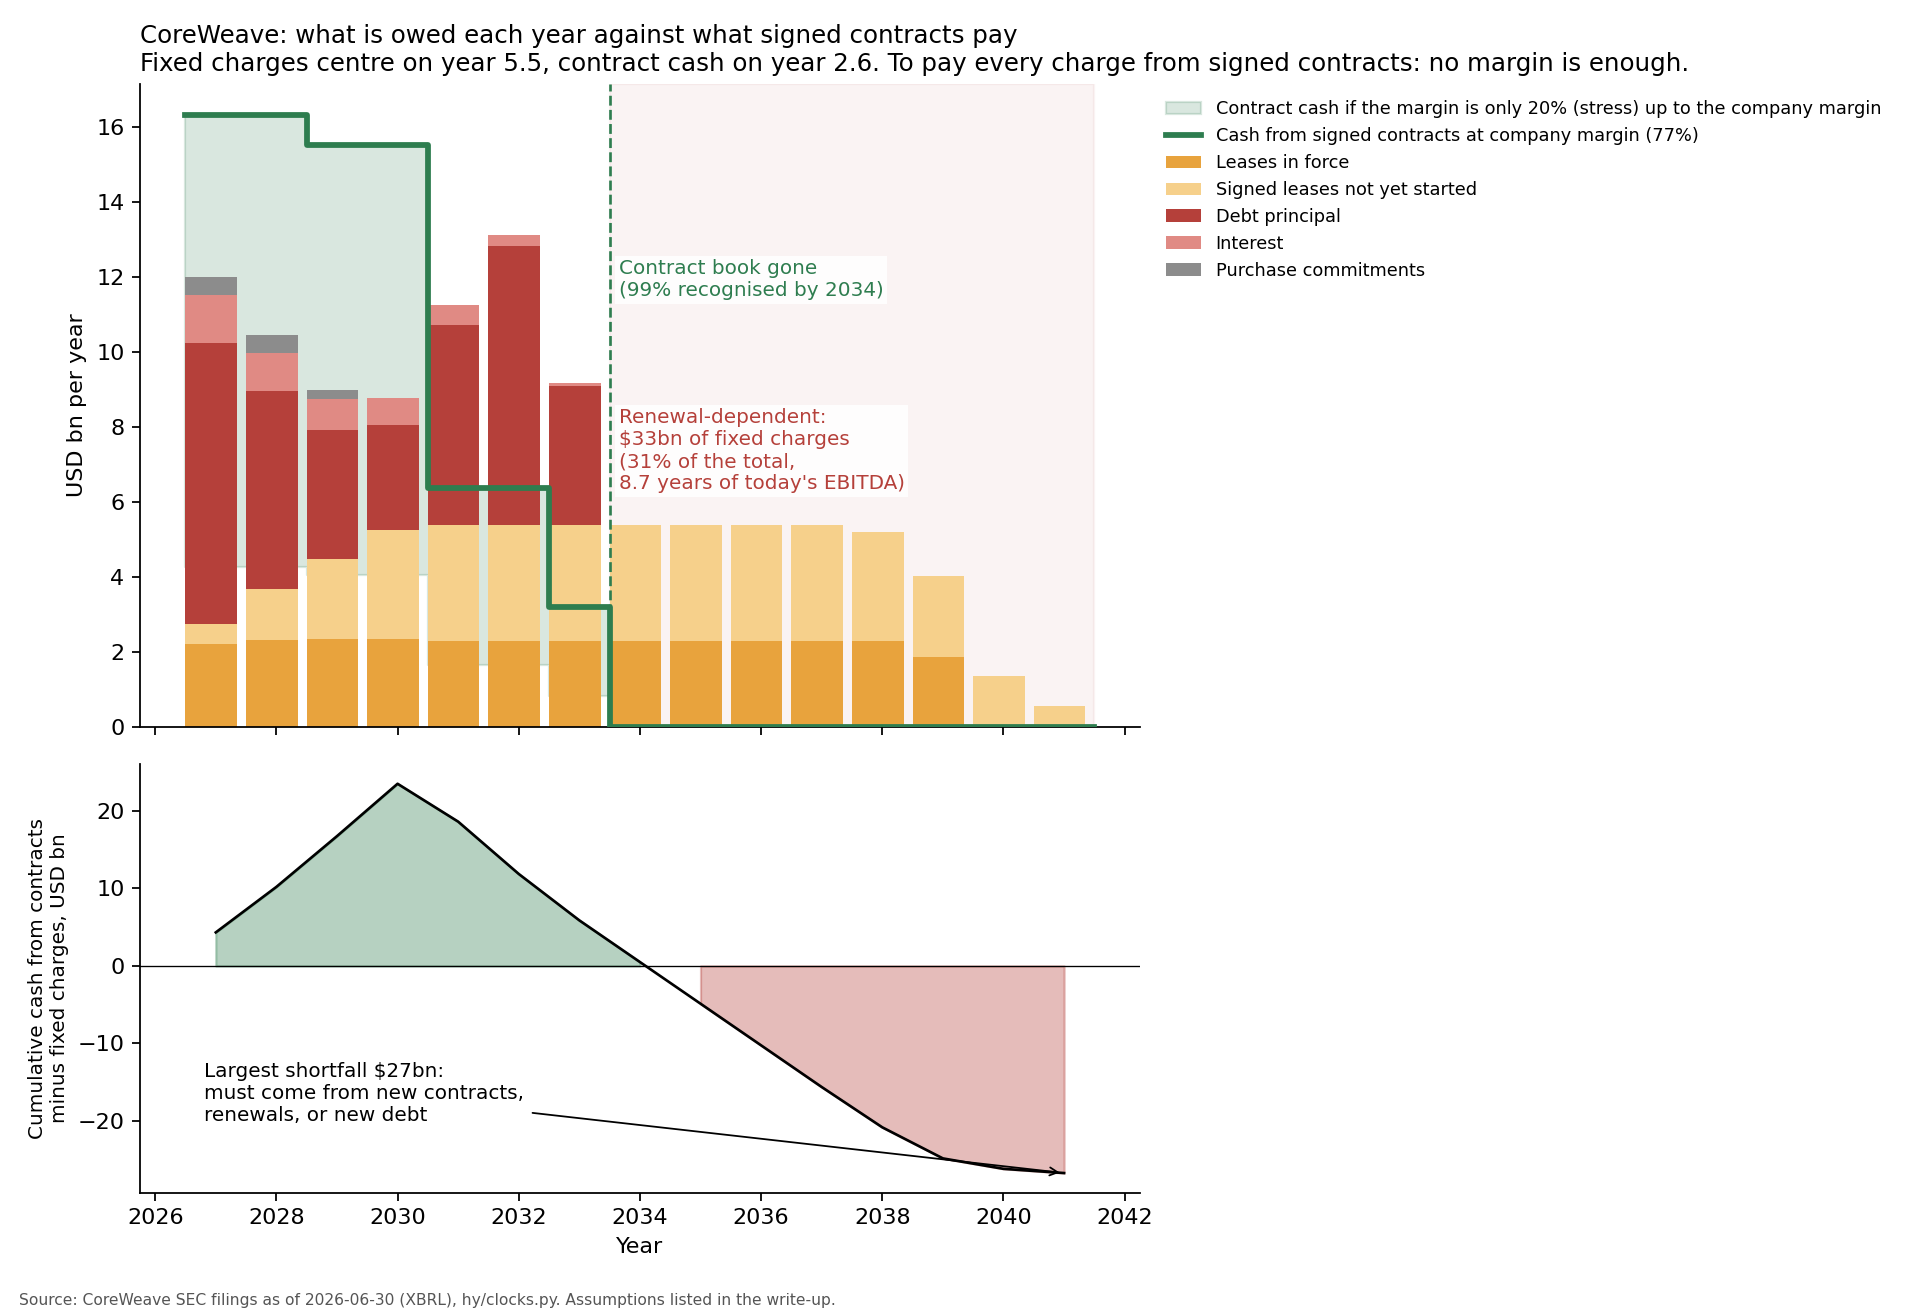
\includegraphics[width=0.95\linewidth]{figures/clocks_all_CRWV.png}\caption*{The two clocks (section G2.1).}\end{figure}
\begin{figure}[H]\centering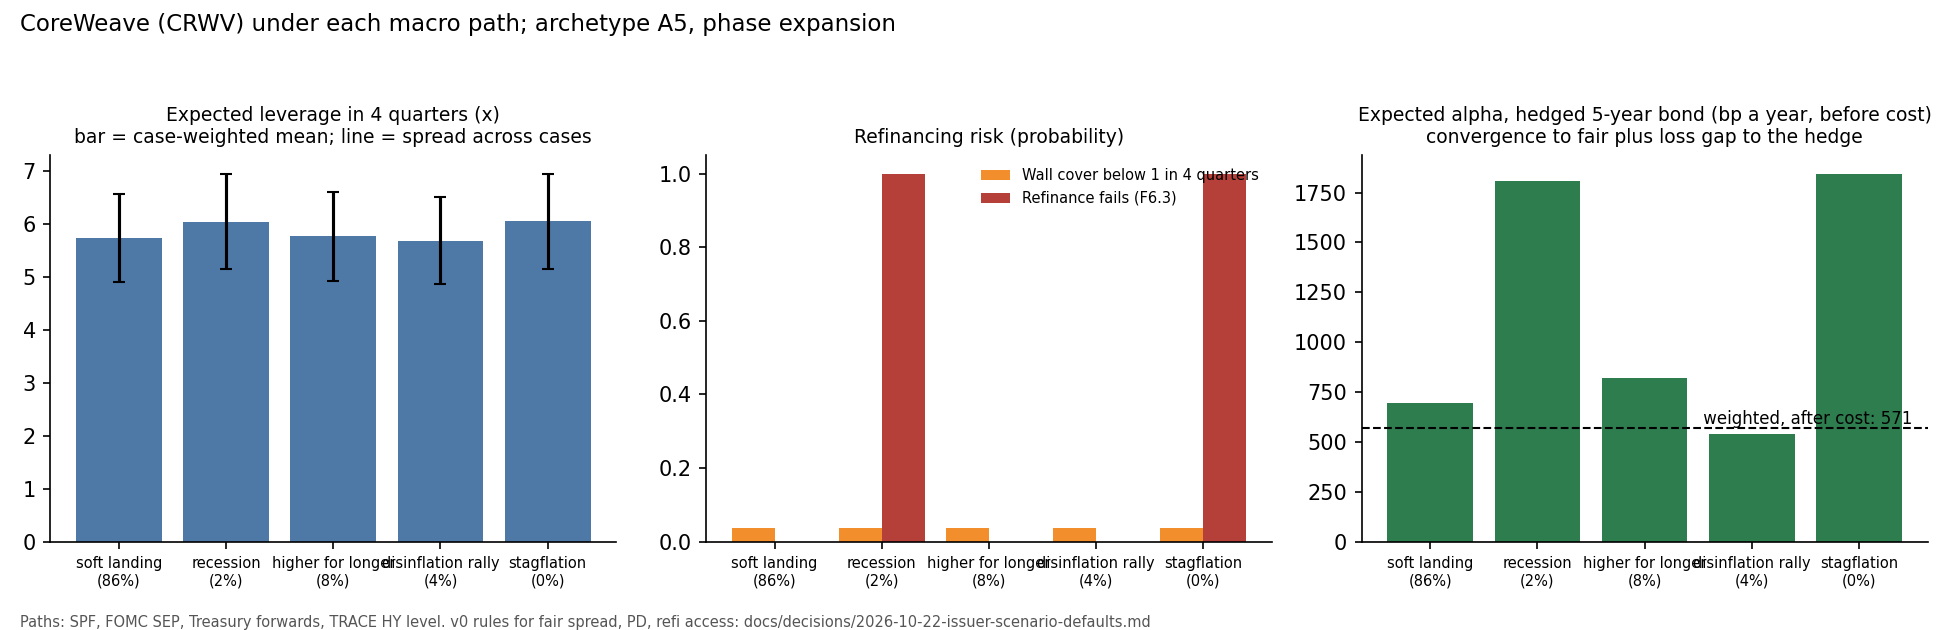
\includegraphics[width=0.95\linewidth]{figures/scenarios_CRWV.png}\caption*{The company under each economic story (section G2.2).}\end{figure}
\begin{figure}[H]\centering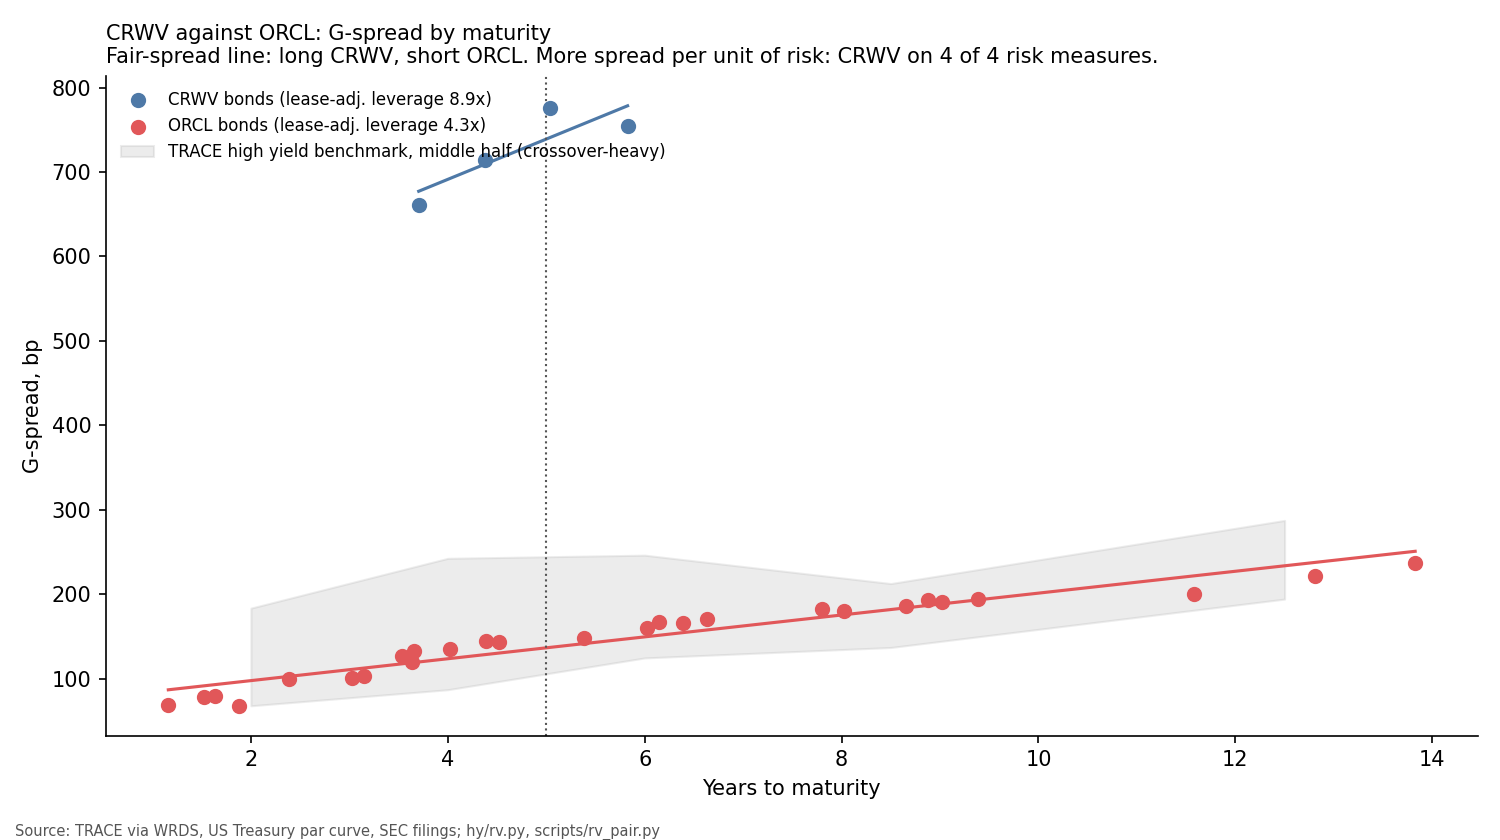
\includegraphics[width=0.85\linewidth]{figures/rv_CRWV_ORCL.png}\caption*{The pair (section G2.3).}\end{figure}
\newpage
\section*{Oracle (ORCL)}\pdfbookmark[1]{ORCL}{bm-ORCL}\label{memo-start-ORCL}
\par\noindent\fcolorbox{gray}{gray!6}{\parbox{\dimexpr\linewidth-2\fboxsep-2\fboxrule-1pt}{\sloppy \textbf{Recommendation.} Pass. This is a view of the company, not a trade: the expected profit does not beat trading costs. If the money went elsewhere, the best alternative in this run is NCLH. Position size and hedge: open until the call passes.}}

\subsection*{The combined view: four groups, one estimate}
Each group of methods estimates the same thing: what the bond should earn above a hedge, in bp a year. The combined estimate weighs the four groups. It ranks 6 of the issuers in this run. 4 of 5 groups point the same way as the combination.
\begin{center}\footnotesize\setlength{\tabcolsep}{3.5pt}\begin{tabular}{@{}lrrrl@{}}\toprule
Group & bp a year & Weight & Adds & Call \\\midrule
G1. Core process & +92 & 45\% & +41 & \textcolor{amber}{leans to owning} \\
G2 clocks. Two clocks & -158 & 20\% & -32 & \textcolor{bad}{against owning} \\
G2 rest. Built methods (rest) & -88 & 12\% & -10 & \textcolor{bad}{against owning} \\
G3. Credit skills & -215 & 12\% & -25 & \textcolor{bad}{against owning} \\
G4. Books & -16 & 12\% & -2 & \textcolor{bad}{against owning} \\
\textbf{Combined, before trading costs} &  &  & \textbf{-27} &  \\
Trading costs &  &  & -173 &  \\
\textbf{Combined, after trading costs} &  &  & \textbf{-201} &  \\
Weighted cases and stories alone, after costs &  &  & -173 &  \\
Calibrated: after-cost number x measured slope 0.079 &  &  & -16 &  \\
\bottomrule\end{tabular}\end{center}
Against the weighted cases and stories alone, the combination is 27 bp a year lower: the other methods take away from the case for owning the bond. A group that supports owning must beat the trading costs on its own. The weights are the user's choice: core process 45\%, two clocks 20\%, and 11.7\% each for the rest of the built methods, the credit skills and the books. The backtest alone would have put most weight on the built methods.
\par\noindent\fcolorbox{gray}{gray!6}{\parbox{\dimexpr\linewidth-2\fboxsep-2\fboxrule-1pt}{\sloppy \textbf{Alpha sizes are uncalibrated.} The backtest (2008 to 2026) shows that this kind of estimate ranks bonds well but overstates the size of the move. Realised alpha has been about 0.08 times the predicted alpha (standard error 0.05; 0.25 since 2019). The calibrated number multiplies by that slope: -16 bp a year after costs (-51 on the 2019 slope). The slope is not above zero by two standard errors, so the number ranks the bond but does not size it. Decision page: 2026-10-22-alpha-backtest-design. The backtest has no default-loss term yet.}}

\section*{G1. Core process: Gatto's steps, our method and rulebook, the relative value paper}
\par\noindent\fcolorbox{gray}{gray!6}{\parbox{\dimexpr\linewidth-2\fboxsep-2\fboxrule-1pt}{\sloppy \textbf{Verdict: \textcolor{amber}{leans to owning}.} This group reads Gatto's seven steps, our method and rulebook, and the relative value paper. Its estimate of expected profit is +92 bp a year before trading costs (costs are 173 bp a year); 3 of 4 of its weighted estimates point the same way. It carries 45\% of the combined view and ranks 2 of the issuers on this group alone. Best alternative for the same money: NCLH.}}
\begin{center}\footnotesize\setlength{\tabcolsep}{3.5pt}\begin{tabular}{@{}p{6.2cm}rrrp{4.2cm}@{}}\toprule
Estimate & bp a year & Weight in group & Adds & Where it comes from \\\midrule
Default chance the price assumes (shown, weight 0) & +6 & 0\% & +0 & F9; mapping C2 \\
Earnings quality, add-backs, FCF check (can only lower) & -167 & 25\% & -42 & F3; ebitda-addback-treatment; hy-model-standards \\
Access to new money and the funding gap & +96 & 25\% & +24 & F4; RV PDF E75-E76 \\
Debt against market value & +297 & 25\% & +74 & F7.7 \\
Return above cash, repriced in every story & +143 & 25\% & +36 & RV PDF E50-E60; C1, C3 \\
\bottomrule\end{tabular}\end{center}
\subsection*{G1.1 Thesis}
The bond pays 136 bp over Treasuries at 5 years. A company with its leverage (4.3x with leases) pays 135 bp on the fair line, so the bond is cheap by 1 bp. The bills outlast the signed contracts (section G2.1), so part of the extra spread pays for a renewal bet that the line does not see. What would reveal it, and when: open question.
\subsection*{G1.2 The business}
\begin{enumerate}
\item \textbf{What it sells:} Oracle provides products and services that build, run and support enterprise information technology (IT) frameworks. Our products and services include enterprise applications and infrastructure offerings that incorporate and are enhanced by artificial intelligence (AI) technologies, including embedded AI-driven automation and analytics and generative AI capabilities.
\item \textbf{How it earns:} revenue 71.8bn a year at a 47\% EBITDA margin.
\item \textbf{What it must spend to stand still:} rent of about \$5.5bn a year, plus maintenance capital spending.
\item \textbf{Competition:} open question.
\item \textbf{What breaks it:} net retention and bookings fall; cost cuts reverse.
\end{enumerate}
Business type: A6.
\subsection*{G1.3 Earnings, normalised}
Last 12 months: EBITDA \$33.9bn at a 47\% margin; margin trend over 8 quarters 3.8 (t-statistic: above 1 rising, below $-1$ falling). One-off items \$-0.6bn. Free cash flow \$-28.7bn: -85\% of EBITDA. Earnings-quality flags raised: EQ7 conversion, EQ5 recurrence, FCF check (waterfall against OCF less capex) (of 5 tests the data supports). The add-back detail is in section G3.1.
\subsection*{G1.4 Cash, the funding gap, and the refinancing shock}
\begin{center}\footnotesize\setlength{\tabcolsep}{3.5pt}\begin{tabular}{@{}lr@{}}\toprule
Item & Value \\\midrule
Cash & \$37.0bn \\
Unused credit lines (tagged) & \$0.0bn \\
Less cash needed to run & \$0.4bn \\
Liquidity & \$36.6bn \\
Runway at today's cash burn, all capital spending (quarters) & 5.1 \\
First quarter cash runs out, severe case, maintenance spending only & no shortfall in 8 quarters \\
First quarter cash runs out, severe case, all committed spending & 2 \\
\textbf{Runway we quote (the shortest)} & \textbf{2.0} (severe, committed capex) \\
Debt due in the next 18 months & \$7.2bn \\
Cash to meet debt due in a year, base case & 7.34x \\
Refinancing access score, likely story (0 to 6) & 3 \\
\bottomrule\end{tabular}\end{center}
\textbf{Funding gap if no lender refinances.} We add cash, the unused lines and the free cash flow of the cases, then take off the debt as it falls due, quarter by quarter. The minimum cash kept back is one month of cash operating costs (\$3.2bn).
\begin{center}\footnotesize\setlength{\tabcolsep}{3.5pt}\begin{tabular}{@{}lr@{}}\toprule
Measure & Value \\\midrule
Lowest point, likely story (maintenance spending only) & \$37.2bn \\
First quarter below zero, likely story & none in 8 quarters \\
Lowest point with all capital spending & \$-148.7bn \\
First quarter below zero with all capital spending & quarter 2 \\
Lowest point, severe case & \$35.1bn \\
Severe case with all capital spending: first quarter below zero & quarter 2 \\
Lowest point, weighted over the stories & \$37.2bn \\
Debt due inside 8 quarters, share of all debt & 14\% \\
\bottomrule\end{tabular}\end{center}
\textbf{Refinancing shock.} \$17.4bn falls due in the next two years. It pays about 3.71\% today (TRACE coupons of bonds due inside 27 months). Refinanced at the forecast Treasury rate plus today's spread, yearly interest changes by \$0.5bn (1.4\% of EBITDA). Interest cover after refinancing: 6.1x; after capital spending -7.5x. Free cash flow after the shock: -23.3\% of debt.
\subsection*{G1.5 Debt: going-concern view}
\begin{center}\footnotesize\setlength{\tabcolsep}{3.5pt}\begin{tabular}{@{}lr@{}}\toprule
Measure & Value \\\midrule
Debt & \$125.3bn \\
Lease liabilities & \$43.8bn \\
EBITDA, last 12 months & \$33.9bn \\
Debt / EBITDA & 3.7x \\
(Debt + leases) / (EBITDA + rent) & 4.3x \\
Net debt / EBITDA & 2.6x \\
Coverage (after all capital spending) & -8.2x \\
Fixed-charge cover (after maintenance spending) & 2.75x \\
\bottomrule\end{tabular}\end{center}
\begin{center}\footnotesize\setlength{\tabcolsep}{3.5pt}\begin{tabular}{@{}lrrrrr@{}}\toprule
Bond & Coupon & Matures & Price & Yield & Spread (bp) \\\midrule
68389XBN4 & 3.25\% & 2027-11-15 & 97.9 & 5.13\% & 69 \\
68389XCD5 & 2.30\% & 2028-03-25 & 95.6 & 5.32\% & 78 \\
68389XCM5 & 4.50\% & 2028-05-06 & 98.6 & 5.37\% & 80 \\
68389XCY9 & 4.80\% & 2028-08-03 & 99.1 & 5.32\% & 68 \\
68389XDW2 & 4.55\% & 2029-02-04 & 97.5 & 5.69\% & 99 \\
68389XCS2 & 4.20\% & 2029-09-27 & 95.7 & 5.76\% & 101 \\
\bottomrule\end{tabular}\end{center}
Claims view (who is paid what in a default): open question until the debt documents are read.
\subsection*{G1.6 Company value}
Market value of the whole company \$540bn (shares \$451bn plus net debt): 15.9x EBITDA; debt is 23\% of it. Our own valuation range and the bonds' recovery if the company defaults: open questions (they need a peer set and a distressed multiple).
\subsection*{G1.7 The decision against cash}
We put the same money in the bond nearest five years (68389XCZ6, 5.25\% due 2032-02-03, price 95.37 plus 0.63 accrued) or in six-month Treasury bills at 4.20\%. In each story the bond either survives and is repriced, or defaults and returns 35 per 100 (a 40\% recovery paid a year later, valued at 15\% a year). In default the holder loses 64\% of the price paid.
\begin{center}\footnotesize\setlength{\tabcolsep}{3.5pt}\begin{tabular}{@{}lr@{}}\toprule
Measure & Value \\\midrule
Expected return above cash, bp a year & +143 \\
Chance of a loss over six months & 9.2\% \\
Chance of doing worse than cash & 9.2\% \\
Average loss in the worst 5\% of outcomes & 7.7\% \\
Same, with rates and the market hedged out, bp a year & -10 \\
Best alternative in this run (worst 5\% loss within the 25\% budget) & NCLH \\
Return given up against that alternative, bp a year & +304 \\
\bottomrule\end{tabular}\end{center}
\section*{G2. Built methods: two clocks, stories and cases, relative value, the gate}
\par\noindent\fcolorbox{gray}{gray!6}{\parbox{\dimexpr\linewidth-2\fboxsep-2\fboxrule-1pt}{\sloppy \textbf{Verdict: \textcolor{bad}{against owning}.} This group reads the spread level, the fair line and the pair, the economic stories, the health panel. Its estimate of expected profit is -88 bp a year before trading costs (costs are 173 bp a year); 4 of 5 of its weighted estimates point the same way. It carries 12\% of the combined view and ranks 8 of the issuers on this group alone. Gate: pass.}}
\begin{center}\footnotesize\setlength{\tabcolsep}{3.5pt}\begin{tabular}{@{}p{6.2cm}rrrp{4.2cm}@{}}\toprule
Estimate & bp a year & Weight in group & Adds & Where it comes from \\\midrule
Spread level: the extra pay over the market (carry) & -31 & 42\% & -13 & Spec S14 E0; K15 \\
Weighted cases and stories & -0 & 25\% & -0 & M5.4, M7.5 \\
Spread against the fair line & +3 & 17\% & +1 & M7.4, M7.5 \\
The pair & -776 & 8\% & -65 & M7.4; F10 S4 \\
Health panel & -130 & 8\% & -11 & F8 \\
\bottomrule\end{tabular}\end{center}
\subsection*{G2.1 The two clocks: bills against what pays for them}
\par\noindent\fcolorbox{gray}{gray!6}{\parbox{\dimexpr\linewidth-2\fboxsep-2\fboxrule-1pt}{\sloppy \textbf{Verdict: \textcolor{bad}{against owning}.} This group reads the bills the company owes against the revenue customers have signed for. Its estimate of expected profit is -158 bp a year before trading costs (costs are 173 bp a year); 1 of 1 of its weighted estimates point the same way. It carries 20\% of the combined view and ranks 7 of the issuers on this group alone. The clocks count as their own bucket in the combined view.}}
\begin{center}\footnotesize\setlength{\tabcolsep}{3.5pt}\begin{tabular}{@{}p{6.2cm}rrrp{4.2cm}@{}}\toprule
Estimate & bp a year & Weight in group & Adds & Where it comes from \\\midrule
The two clocks & -158 & 100\% & -158 & M4.7 \\
\bottomrule\end{tabular}\end{center}
Fixed bills total \$549.0bn, centred 8.2 years out: leases in force \$63.2bn, signed leases not yet started \$288.0bn, debt principal \$130.1bn, interest \$33.5bn, purchase commitments \$34.1bn. That is 13.9 years of today's EBITDAR; next year's bills take 75\% of it.
\begin{center}\footnotesize\setlength{\tabcolsep}{3.5pt}\begin{tabular}{@{}lr@{}}\toprule
Measure & Value \\\midrule
Signed contracts (RPO) & \$664.0bn \\
Where bills centre / where contract cash centres & year 8.2 / year 3.4 \\
Contracts 99\% booked by & year 10 \\
Margin needed for contracts to pay every bill & 83\% \\
Company margin (EBITDAR) & 55\% \\
Share of bills paid by contracts at that margin & 66\% \\
Bills due after the contracts end & \$203.8bn (37\%) \\
\quad of which debt to refinance & \$46.4bn (8\%) \\
\quad of which rent and purchases to recontract & \$157.4bn (29\%) \\
Revenue to sign after the contracts end & 4.8 years of today's revenue \\
Largest running shortfall & \$184.8bn \\
Top three customers & n/a \\
Share paid by contracts at a 0.20 margin & 24\% \\
Share paid by contracts at a 0.35 margin & 42\% \\
Share paid by contracts at a 0.50 margin & 60\% \\
Share paid by contracts at a 0.55 margin & 67\% \\
\bottomrule\end{tabular}\end{center}
\subsection*{G2.2 Economic stories and cases}
Cases on the most likely story (soft landing), stage of the cycle: expansion.
\begin{center}\scriptsize\setlength{\tabcolsep}{3.5pt}\begin{tabular}{@{}lrrrrrrr@{}}\toprule
Case & Weight & Growth / qtr & Leverage in 1 yr & Peak leverage & Lowest liquidity & Cash runs out & Refi fails \\\midrule
base & 60\% & 5.0\% & 3.0x & 3.5x & \$40.4bn & no & no \\
down moderate & 15\% & 3.3\% & 3.2x & 3.5x & \$40.6bn & no & no \\
down severe & 5\% & 2.3\% & 4.3x & 4.3x & \$39.1bn & no & no \\
upside & 20\% & 6.6\% & 2.8x & 3.4x & \$40.3bn & no & no \\
\bottomrule\end{tabular}\end{center}
\begin{center}\scriptsize\setlength{\tabcolsep}{3.5pt}\begin{tabular}{@{}lrrrrrr@{}}\toprule
Story & Chance & Leverage in 1 yr & Peak leverage (down) & Refi fails & Default chance & Expected profit (bp/yr) \\\midrule
soft landing & 86\% & 3.1x & 4.3x & 0\% & 0.9\% & -0 \\
recession & 2\% & 3.2x & 4.4x & 0\% & 2.4\% & 0 \\
higher for longer & 8\% & 3.1x & 4.3x & 0\% & 1.1\% & -0 \\
disinflation rally & 4\% & 3.1x & 4.2x & 0\% & 0.7\% & -0 \\
stagflation & 0\% & 3.2x & 4.4x & 0\% & 2.5\% & 0 \\
\bottomrule\end{tabular}\end{center}
\subsection*{G2.3 Relative value and the pair}
Fair line: log spread = -5.64 + 0.312 x leverage, fitted on 8 issuers in this run. 5-year spread 136 bp against a fair 135 bp.
\textbf{Against peers.} Peers are the high yield bonds that traded in 2026-08-31 (733 bonds with leverage on file), in the same 3 to 7 year maturity bucket. Sector: Information Technology. Rating class: BB (implied by leverage). A positive value means the issuer pays more than the median peer.
\begin{center}\footnotesize\setlength{\tabcolsep}{3.5pt}\begin{tabular}{@{}lrr@{}}\toprule
Peer group & Excess spread to peers (ESP) & Spread per turn against peers (E13) \\\midrule
Sector and rating & -5\% & -12\% \\
Sector only & -3\% & -5\% \\
Rating only & -5\% & -12\% \\
\bottomrule\end{tabular}\end{center}
The sector and rating cell has fewer than five other issuers, so that row uses the rating cell.
\textbf{SPiDER} (spread per unit of debt to 10-year average EBITDA; Dynkin et al. 2021, ch. 14): cheaper than 32\% of the peer bonds across all sectors, and -40\% against sector and rating peers. It has no weight in the score: its edge beyond spread level is small (t 1.3 at 12 months).
\textbf{Against CRWV.} Spreads at 5 years: CRWV 739 bp, ORCL 136 bp.
\begin{center}\footnotesize\setlength{\tabcolsep}{3.5pt}\begin{tabular}{@{}lrrr@{}}\toprule
Spread per & CRWV & ORCL & Cheaper \\\midrule
turn of leverage & 83 & 32 & CRWV \\
year of EBITDA that depends on renewal & 85 & 23 & CRWV \\
unit of breakeven margin & 721 & 165 & CRWV \\
year of clock gap & 257 & 28 & CRWV \\
\bottomrule\end{tabular}\end{center}
The fair line favours long CRWV, short ORCL: a gap of 159 bp, which halves in about 17 weeks on six months of trades. Under the stories the pair earns soft landing +348, recession +918, higher for longer +414, disinflation rally +270, stagflation +935 bp a year; weighted +363 bp before costs.
\subsection*{G2.4 Expected profit and price against our view}
Hedged 5-year bond over six months: -0 bp a year before trading costs, -173 bp after. It does not beat costs. The expected default loss is charged on the price paid: 64\% of it in default, not 60\% of face.
\begin{center}\footnotesize\setlength{\tabcolsep}{3.5pt}\begin{tabular}{@{}p{5.2cm}rrrrl@{}}\toprule
Question & Price assumes & Our view & Gap & Noise & Gap bigger than noise? \\\midrule
Default chance at the v0 price of risk (shown, not tested) & 1.1\% & 1.0\% & -0.1\% & open & not tested \\
Breakeven default probability, 12 months (loss on price) & 2.1\% & 1.0\% & -1.2\% & 1.1\% & yes \\
Leverage the spread is pricing & 4.33 & 4.30 & -0.03 & 0.90 & no \\
Spread against fair (bp) & 136 & 135 & -1 & 38 & no \\
Rating class & open & BBB & open & open & not tested \\
Recovery if default (per 1 of face, discounted for delay) & open & 0.35 & open & open & not tested \\
\bottomrule\end{tabular}\end{center}
The first row turns the spread into a default chance with a fixed price of risk. That is not a real default chance, so it is shown but not tested. The breakeven row asks a cleaner question: is our default chance below the rate at which the spread only just pays for default losses?
\subsection*{G2.5 Risks and the health panel}
\begin{itemize}\item Earnings after capital spending do not cover interest. Tracked by: coverage (-8.19). Resolves when: capital spending falls, or earnings rise.\item Little of the earnings turns into free cash. Tracked by: cash conversion (fcf / ebitda) (-0.85). Resolves when: growth spending ends.\item Free cash flow repays little debt. Tracked by: free cash flow / debt (-0.23). Resolves when: free cash flow turns positive.\item Earnings-quality flags are raised. Tracked by: earnings-quality flags (3.00). Resolves when: flags clear in the next two quarters.\end{itemize}
\begin{center}\footnotesize\setlength{\tabcolsep}{3.5pt}\begin{tabular}{@{}lrl@{}}\toprule
Measure & Value & Band \\\midrule
Coverage & -8.19 & \textcolor{bad}{red} \\
Cash conversion (FCF / EBITDA) & -0.85 & \textcolor{bad}{red} \\
Free cash flow / debt & -0.23 & \textcolor{bad}{red} \\
Earnings-quality flags & 3.00 & \textcolor{bad}{red} \\
Refinancing access score (0 to 6) & 3.00 & \textcolor{amber}{amber} \\
Fixed-charge cover & 2.75 & \textcolor{good}{green} \\
Cash to meet debt due in 1 year (base case) & 7.34 & \textcolor{good}{green} \\
Margin trend (t-statistic) & 3.77 & \textcolor{good}{green} \\
Weight on the downside cases & 0.20 & \textcolor{good}{green} \\
Chance debt due in 1 year is not covered & 0.00 & \textcolor{good}{green} \\
Chance cash runs out within 2 years & 0.00 & \textcolor{good}{green} \\
\bottomrule\end{tabular}\end{center}
\section*{G3. Credit skills: the lender's checklists applied to a public bond}
\par\noindent\fcolorbox{gray}{gray!6}{\parbox{\dimexpr\linewidth-2\fboxsep-2\fboxrule-1pt}{\sloppy \textbf{Verdict: \textcolor{bad}{against owning}.} This group reads the lender's checklists: add-backs, covenants, watchlist, trend, memo structure. Its estimate of expected profit is -215 bp a year before trading costs (costs are 173 bp a year); 1 of 1 of its weighted estimates point the same way. It carries 12\% of the combined view and ranks 6 of the issuers on this group alone. Its estimates can only lower the combined number: a clean checklist earns no credit. Watchlist: watchlist.}}
\begin{center}\footnotesize\setlength{\tabcolsep}{3.5pt}\begin{tabular}{@{}p{6.2cm}rrrp{4.2cm}@{}}\toprule
Estimate & bp a year & Weight in group & Adds & Where it comes from \\\midrule
Watchlist tier (can only lower) & -215 & 100\% & -215 & borrower-monitoring; covenant-compliance \\
\bottomrule\end{tabular}\end{center}
\subsection*{G3.1 Add-backs and their cash effect}
Reported EBITDA over the last 12 months is \$33.3bn. The company's own measure adds back \$0.6bn of one-off items to reach \$33.9bn: 1.7\% of reported EBITDA (a negative figure is a one-off gain taken out). This is under the 5\% line for one item. They do not recur in three quarters running. If every add-back were paid in cash, free cash flow would be \$-29.3bn. The two roads to free cash flow (the EBITDA bridge, \$-49.4bn; operating cash flow less capital spending, \$-28.7bn) differ by 61\% of EBITDA: above the 10\% tolerance, so an earnings-quality flag is raised. The add-back table by category is an open question: the data has one total line.
\subsection*{G3.2 Covenant headroom}
The 10-Q and 10-K text state no maintenance test level. Public bonds are often tested only when the company borrows more or pays out cash. Headroom is an open question until the credit agreement is read.
\subsection*{G3.3 Watchlist and trajectory}
Watchlist tier: \textbf{watchlist} because free cash flow is negative. EBITDA against the same months a year earlier: 38.3\% (no plan is public, so last year stands in for it).
\begin{center}\footnotesize\setlength{\tabcolsep}{3.5pt}\begin{tabular}{@{}llll@{}}\toprule
Measure & Direction & How much weight & Change on a year earlier, last quarter \\\midrule
revenue & improving & trend & 29.6\% \\
EBITDA & improving & trend & 53.1\% \\
EBITDA margin & improving & trend & 18.1\% \\
cash conversion & deteriorating & observation & -873.5\% \\
\bottomrule\end{tabular}\end{center}
One quarter is an observation, two a data point, three or four a trend. The measures point different ways; the memo must explain why.
\subsection*{G3.4 Memo structure check}
\begin{center}\footnotesize\setlength{\tabcolsep}{3.5pt}\begin{tabular}{@{}lp{9cm}l@{}}\toprule
Section & Requires & Status \\\midrule
Executive summary & the business in one sentence, the opportunity, 2 to 3 reasons, 2 to 3 risks & \textcolor{good}{pass} \\
Capital structure & each tranche with face, coupon, maturity; senior, total and net leverage; LTV & \textcolor{amber}{open} \\
Terms & maintenance covenant levels and test dates; incurrence baskets; call terms & \textcolor{amber}{open} \\
Investment merits & free cash flow generation and the base-case deleveraging path & \textcolor{good}{pass} \\
Key risks & 3 to 5 issuer-specific risks, each with a mitigant & \textcolor{good}{pass} \\
Historical financials & at least 3 years, quarterly where available & \textcolor{good}{pass} \\
EBITDA adjustments & reported-to-adjusted bridge with the load as a share of EBITDA and the 5\% flag & \textcolor{amber}{open} \\
Model output & base and downside: EBITDA, FCF, leverage path, covenant headroom, liquidity runway & \textcolor{amber}{open} \\
\bottomrule\end{tabular}\end{center}
\textbf{Rules that do not transfer to a public bond:}\begin{itemize}\item The compliance certificate is the source of truth; public bonds have none. Headroom here uses our own ratio against a level parsed from the filing text. (covenant-compliance)\item Equity cures, step-down schedules and window-dressing checks need the credit agreement and monthly revolver balances. (covenant-compliance)\item Performance against the sponsor plan: no plan is public. The proxy is the same quarters a year earlier. (borrower-monitoring)\item Add-back caps and the certificate reconciliation live in the credit agreement. Compustat gives one special-items line, not the category table. (ebitda-addback-treatment)\item Sources and uses at entry, the sponsor case and the management call apply to new loans, not to bonds bought in the secondary market. (credit-memo-standards)\item Monthly lender packages do not exist for public issuers; XBRL quarters replace them. (quarterly-package-extraction)\end{itemize}
\section*{G4. Books: Kricheff, and Ganguin and Bilardello (S\&P)}
\par\noindent\fcolorbox{gray}{gray!6}{\parbox{\dimexpr\linewidth-2\fboxsep-2\fboxrule-1pt}{\sloppy \textbf{Verdict: \textcolor{bad}{against owning}.} This group reads Kricheff's cash bridge and ratios; the S\&P risk profiles and rating anchor. Its estimate of expected profit is -16 bp a year before trading costs (costs are 173 bp a year); 1 of 2 of its weighted estimates point the same way. It carries 12\% of the combined view and ranks 5 of the issuers on this group alone. S\&P anchor class: BBB.}}
\begin{center}\footnotesize\setlength{\tabcolsep}{3.5pt}\begin{tabular}{@{}p{6.2cm}rrrp{4.2cm}@{}}\toprule
Estimate & bp a year & Weight in group & Adds & Where it comes from \\\midrule
Spread against the S\&P risk score & -31 & 50\% & -16 & Ganguin and Bilardello ch. 10 \\
Spread per turn of leverage (with the trap guard) & +0 & 50\% & +0 & Kricheff ch. 21 \\
\bottomrule\end{tabular}\end{center}
\subsection*{G4.1 Kricheff's cash-flow bridge and ratio set}
\begin{center}\footnotesize\setlength{\tabcolsep}{3.5pt}\begin{tabular}{@{}lr@{}}\toprule
Line (last 12 months) & Value \\\midrule
Adjusted EBITDA & \$33.9bn \\
less capital spending & \$75.7bn \\
less cash interest & \$5.1bn \\
less cash taxes & \$2.8bn \\
less increase in working capital & \$-0.3bn \\
\textbf{Free cash flow} & \textbf{\$-49.4bn} \\
Check: free cash flow before capital spending less operating cash flow & \$-20.7bn \\
Free cash flow after dividends & open (dividends not loaded) \\
\bottomrule\end{tabular}\end{center}
\begin{center}\footnotesize\setlength{\tabcolsep}{3.5pt}\begin{tabular}{@{}lrlr@{}}\toprule
Ratio & Value & Ratio & Value \\\midrule
EBITDA / cash interest & 6.6x & Debt / EBITDA & 3.7x \\
(EBITDA $-$ capex) / interest & -8.2x & Net debt / EBITDA & 2.6x \\
(EBITDA $-$ maintenance capex) / interest & 4.6x & Free cash flow / debt & -23.0\% \\
EBITDA / debt (highest rate at 1x cover) & 27.0\% & Market value / EBITDA & 15.9x \\
Equity cushion (1 $-$ debt / market value) & 77\% & Spread per turn of leverage & 37 bp \\
\bottomrule\end{tabular}\end{center}
Kricheff's snapshot rule: operating cash flow does not cover capital spending, so the issuer lives on the capital markets and needs the detailed liquidity work of section G1.4. Spread per turn compares the bond with the run's median of 38 bp a turn. Kricheff warns that a high spread per turn can mean weak cash flow, not value; read it with free cash flow / debt. The book measures leverage through each bond's rank; with no face by rank, total leverage stands in.
\subsection*{G4.2 The S\&P risk profiles and the rating anchor}
S\&P adds leases to debt and scores each ratio against the median of each rating class (CreditStats 2002, from the book). Scores run from 1 (safest) to 10 (default).
\begin{center}\footnotesize\setlength{\tabcolsep}{3.5pt}\begin{tabular}{@{}lrrrr@{}}\toprule
Ratio & Value & Score & BB median & B median \\\midrule
Debt / (debt + market value of equity) & 27\% & 1.2 & 57.5\% & 78.5\% \\
Funds from operations / debt & 28\% & 6.1 & 19.5\% & 10.8\% \\
Free operating cash flow / debt & -17\% & 10.0 & 8.5\% & 2.5\% \\
EBITDA / interest (with lease interest) & 4.0x & 6.8 & 3.2x & 1.8x \\
EBITDA margin & 47\% & 3.0 &  &  \\
\bottomrule\end{tabular}\end{center}
Financial risk score 5.9. Business risk score 5.0: industry 5, steadiness of sales 5 (year-on-year growth varies by 7.8\%), customer spread 5. The book puts 45\% of the weight on business risk for this class, so the default risk score is 5.5: the \textbf{BBB} class. The line from score to spread across the run did not slope upward, so it gives no estimate. The 2005 edition has no modern anchor table; its own weighting table stands in for it.
\section*{Coming events, open questions, and the record}
\begin{itemize}\item Next quarterly results (estimated from filing cadence): 2026-12-12 (estimate).\item Debt due by 1.0 years out:  - \$7.2bn.\end{itemize}
\textbf{Open questions, most important first:}\begin{enumerate}\item A dated catalyst that would close the gap (G2).\item The observable and level that would prove the call wrong (G8).\item Face amount of each tranche and the secured debt ahead of the bonds (debt note table).\item Claims view: allowed claims by class and the entity map (framework F5).\item Maintenance covenant levels: none stated in the 10-Q or 10-K text; read the credit agreement exhibit (public bonds are often incurrence-only).\item Revolver commitment, draw, and borrowing base: not tagged; read the credit agreement note.\item F4 points 3 (unencumbered assets) and 6 (sponsor support) are scored 0 until read.\item Recovery, delay and the required return on a defaulted claim are v0 (R = 0.4, tau = 1 year, k = 15\%); the claims view and documents replace them.\item Peer set of at least four issuers of the same archetype (F3.3) for the valuation range (F7.1).\item Distressed multiple (F7.3) and the recovery of the bonds if the company defaults (F7.9).\end{enumerate}
\textbf{Record (filled at exit):} exit date; return against the rating-matched index; worst point against the index; reason; the rule that would have helped.
\newpage
\begin{figure}[H]\centering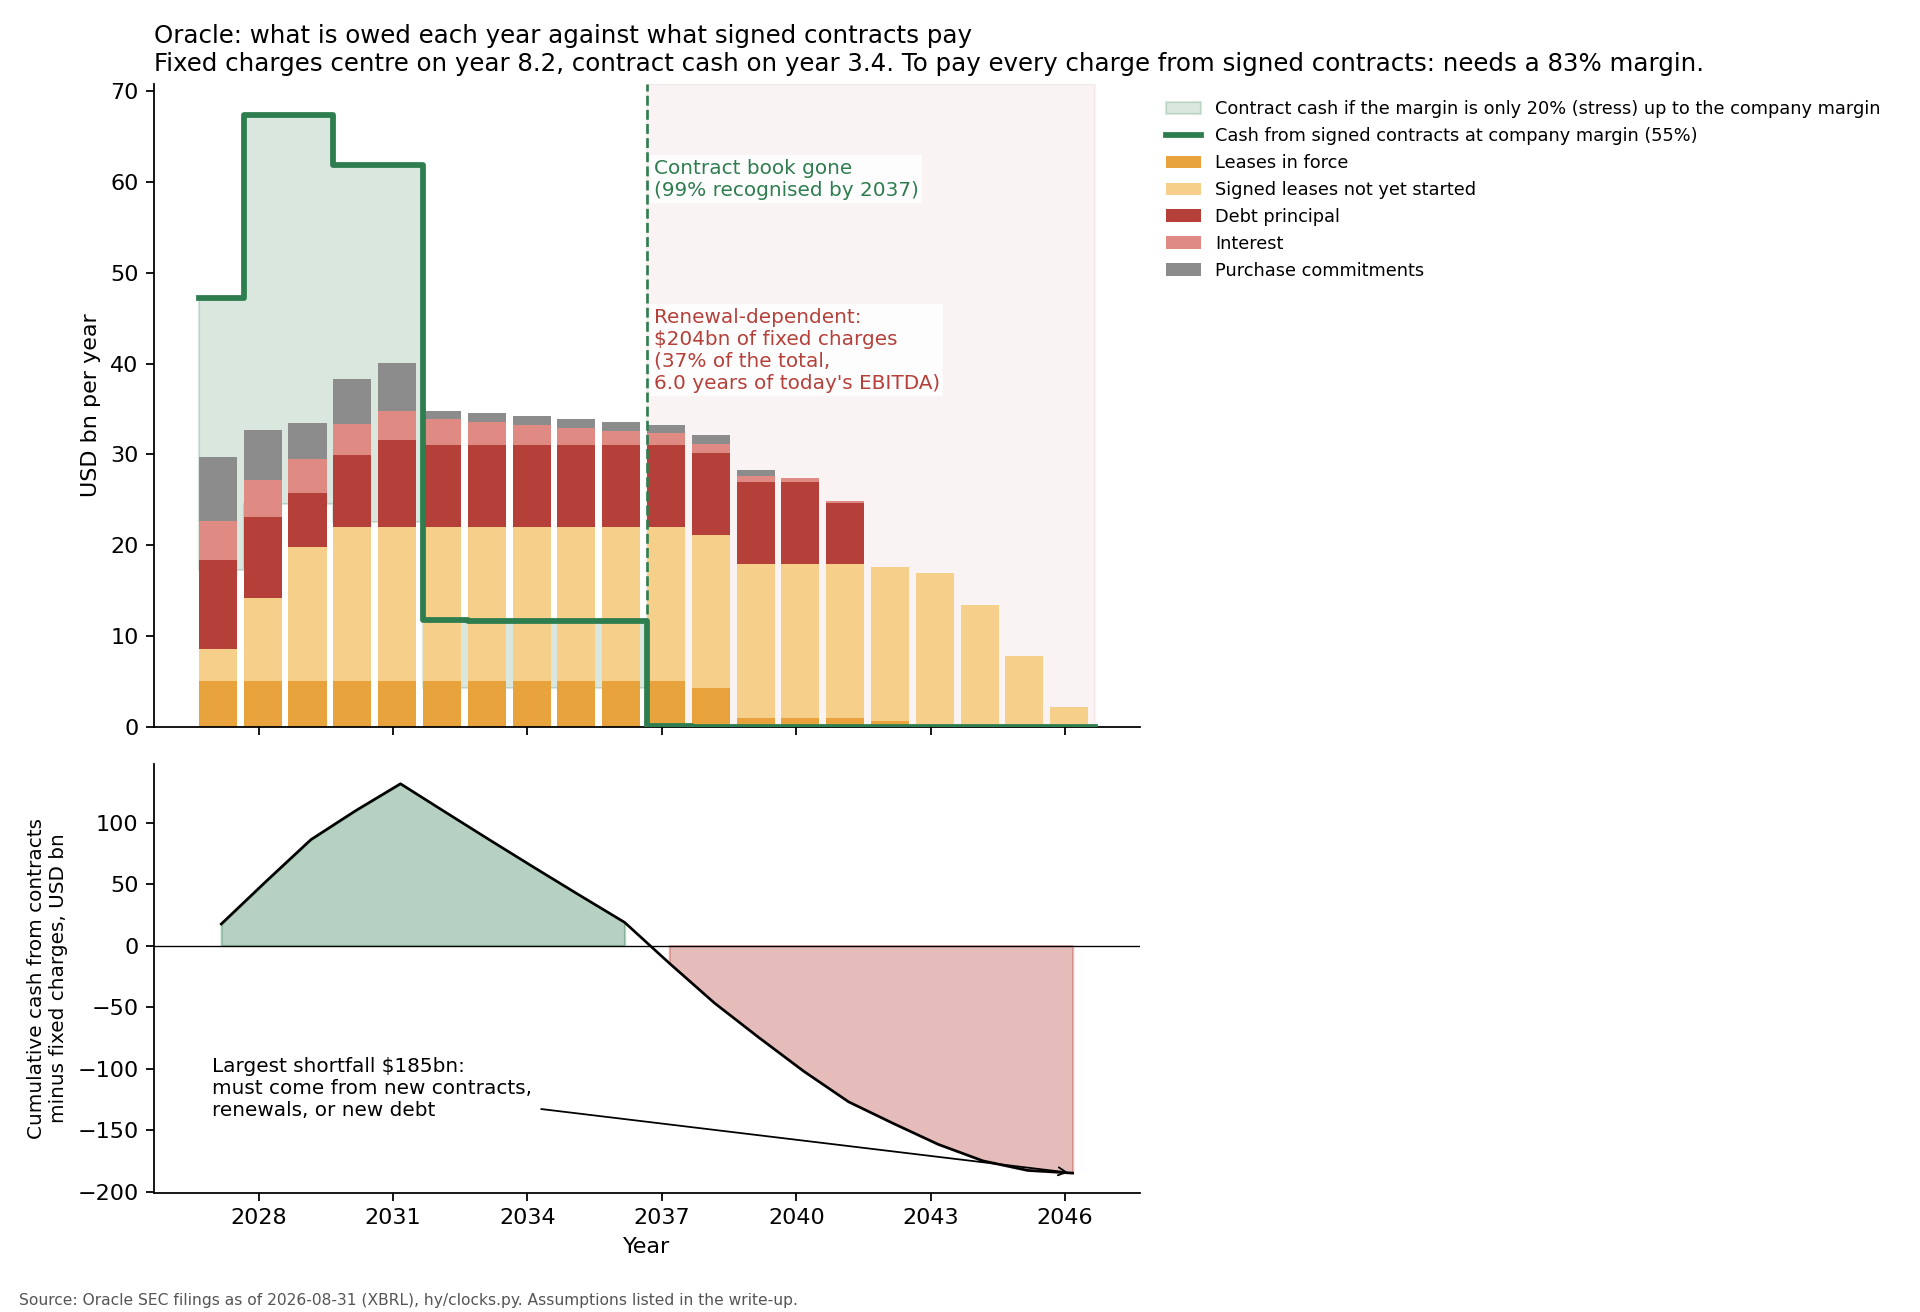
\includegraphics[width=0.95\linewidth]{figures/clocks_all_ORCL.png}\caption*{The two clocks (section G2.1).}\end{figure}
\begin{figure}[H]\centering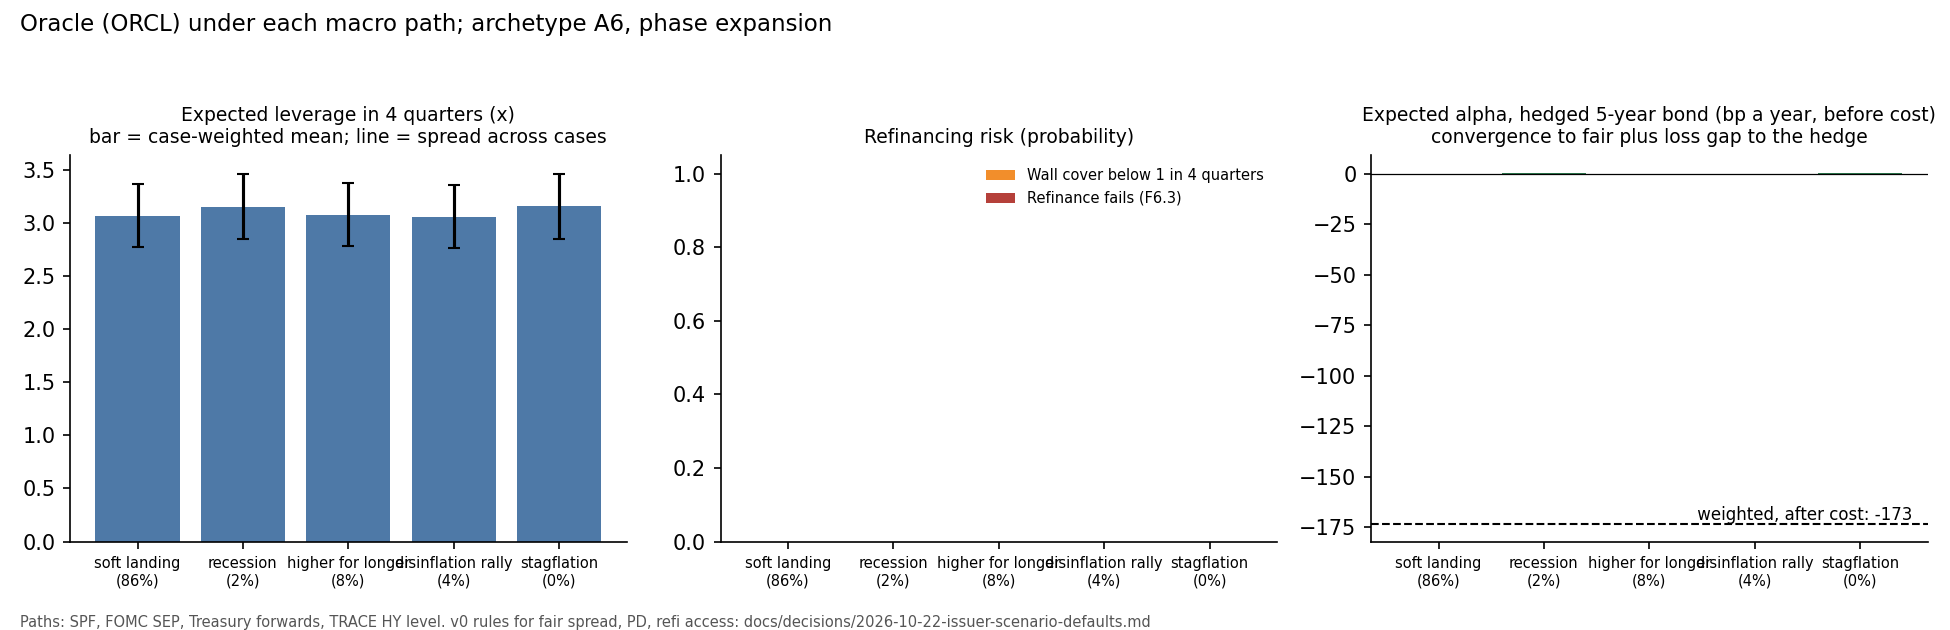
\includegraphics[width=0.95\linewidth]{figures/scenarios_ORCL.png}\caption*{The company under each economic story (section G2.2).}\end{figure}
\begin{figure}[H]\centering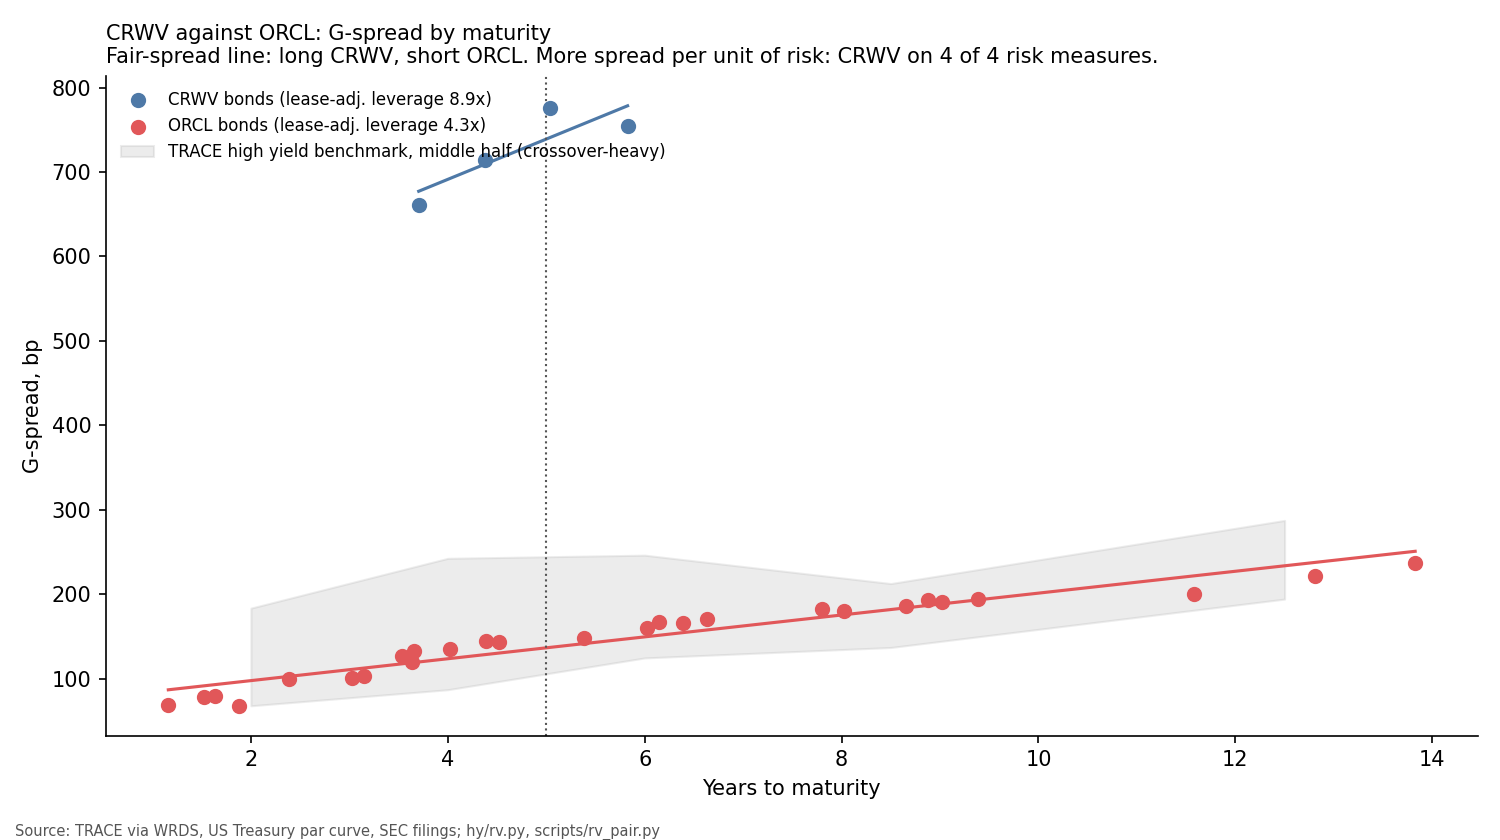
\includegraphics[width=0.85\linewidth]{figures/rv_CRWV_ORCL.png}\caption*{The pair (section G2.3).}\end{figure}
\newpage
\section*{HCA Healthcare (HCA)}\pdfbookmark[1]{HCA}{bm-HCA}\label{memo-start-HCA}
\par\noindent\fcolorbox{gray}{gray!6}{\parbox{\dimexpr\linewidth-2\fboxsep-2\fboxrule-1pt}{\sloppy \textbf{Recommendation.} Pass. This is a view of the company, not a trade: no gap between price and our view is bigger than the noise; the expected profit does not beat trading costs; the checks point in different directions. If the money went elsewhere, the best alternative in this run is NCLH. Position size and hedge: open until the call passes.}}

\subsection*{The combined view: four groups, one estimate}
Each group of methods estimates the same thing: what the bond should earn above a hedge, in bp a year. The combined estimate weighs the four groups. It ranks 4 of the issuers in this run. 2 of 5 groups point the same way as the combination.
\begin{center}\footnotesize\setlength{\tabcolsep}{3.5pt}\begin{tabular}{@{}lrrrl@{}}\toprule
Group & bp a year & Weight & Adds & Call \\\midrule
G1. Core process & +47 & 45\% & +21 & \textcolor{amber}{leans to owning} \\
G2 clocks. Two clocks & +197 & 20\% & +39 & \textcolor{good}{supports owning} \\
G2 rest. Built methods (rest) & -82 & 12\% & -10 & \textcolor{bad}{against owning} \\
G3. Credit skills & +0 & 12\% & +0 & \textcolor{good}{no objection} \\
G4. Books & -113 & 12\% & -13 & \textcolor{bad}{against owning} \\
\textbf{Combined, before trading costs} &  &  & \textbf{+38} &  \\
Trading costs &  &  & -176 &  \\
\textbf{Combined, after trading costs} &  &  & \textbf{-139} &  \\
Weighted cases and stories alone, after costs &  &  & -231 &  \\
Calibrated: after-cost number x measured slope 0.079 &  &  & -11 &  \\
\bottomrule\end{tabular}\end{center}
Against the weighted cases and stories alone, the combination is 92 bp a year higher: the other methods add to the case for owning the bond. A group that supports owning must beat the trading costs on its own. The weights are the user's choice: core process 45\%, two clocks 20\%, and 11.7\% each for the rest of the built methods, the credit skills and the books. The backtest alone would have put most weight on the built methods.
\par\noindent\fcolorbox{gray}{gray!6}{\parbox{\dimexpr\linewidth-2\fboxsep-2\fboxrule-1pt}{\sloppy \textbf{Alpha sizes are uncalibrated.} The backtest (2008 to 2026) shows that this kind of estimate ranks bonds well but overstates the size of the move. Realised alpha has been about 0.08 times the predicted alpha (standard error 0.05; 0.25 since 2019). The calibrated number multiplies by that slope: -11 bp a year after costs (-35 on the 2019 slope). The slope is not above zero by two standard errors, so the number ranks the bond but does not size it. Decision page: 2026-10-22-alpha-backtest-design. The backtest has no default-loss term yet.}}

\section*{G1. Core process: Gatto's steps, our method and rulebook, the relative value paper}
\par\noindent\fcolorbox{gray}{gray!6}{\parbox{\dimexpr\linewidth-2\fboxsep-2\fboxrule-1pt}{\sloppy \textbf{Verdict: \textcolor{amber}{leans to owning}.} This group reads Gatto's seven steps, our method and rulebook, and the relative value paper. Its estimate of expected profit is +47 bp a year before trading costs (costs are 176 bp a year); 2 of 4 of its weighted estimates point the same way. It carries 45\% of the combined view and ranks 4 of the issuers on this group alone. Best alternative for the same money: NCLH.}}
\begin{center}\footnotesize\setlength{\tabcolsep}{3.5pt}\begin{tabular}{@{}p{6.2cm}rrrp{4.2cm}@{}}\toprule
Estimate & bp a year & Weight in group & Adds & Where it comes from \\\midrule
Default chance the price assumes (shown, weight 0) & -6 & 0\% & -0 & F9; mapping C2 \\
Earnings quality, add-backs, FCF check (can only lower) & +0 & 25\% & +0 & F3; ebitda-addback-treatment; hy-model-standards \\
Access to new money and the funding gap & +96 & 25\% & +24 & F4; RV PDF E75-E76 \\
Debt against market value & +124 & 25\% & +31 & F7.7 \\
Return above cash, repriced in every story & -32 & 25\% & -8 & RV PDF E50-E60; C1, C3 \\
\bottomrule\end{tabular}\end{center}
\subsection*{G1.1 Thesis}
The bond pays 68 bp over Treasuries at 5 years. A company with its leverage (2.9x with leases) pays 88 bp on the fair line, so the bond is expensive by 20 bp. What would reveal it, and when: open question.
\subsection*{G1.2 The business}
\begin{enumerate}
\item \textbf{What it sells:} HCA Healthcare, Inc. is one of the leading health care services companies in the United States. At December 31, 2025, we operated 190 hospitals, comprised of 179 general acute care hospitals, seven behavioral hospitals, and four rehabilitation hospitals.
\item \textbf{How it earns:} revenue 76.4bn a year at a 20\% EBITDA margin.
\item \textbf{What it must spend to stand still:} rent of about \$0.0bn a year, plus maintenance capital spending.
\item \textbf{Competition:} open question.
\item \textbf{What breaks it:} a reimbursement rule change, bad debt, or labour cost inflation.
\end{enumerate}
Business type: A2.
\subsection*{G1.3 Earnings, normalised}
Last 12 months: EBITDA \$15.6bn at a 20\% margin; margin trend over 8 quarters 1.3 (t-statistic: above 1 rising, below $-1$ falling). One-off items \$0.0bn. Free cash flow \$7.9bn: 51\% of EBITDA. Earnings-quality flags raised: none (of 4 tests the data supports). The add-back detail is in section G3.1.
\subsection*{G1.4 Cash, the funding gap, and the refinancing shock}
\begin{center}\footnotesize\setlength{\tabcolsep}{3.5pt}\begin{tabular}{@{}lr@{}}\toprule
Item & Value \\\midrule
Cash & \$1.1bn \\
Unused credit lines (tagged) & \$0.0bn \\
Less cash needed to run & \$0.4bn \\
Liquidity & \$0.7bn \\
Runway at today's cash burn, all capital spending (quarters) & no burn \\
First quarter cash runs out, severe case, maintenance spending only & no shortfall in 8 quarters \\
First quarter cash runs out, severe case, all committed spending & no shortfall in 8 quarters \\
\textbf{Runway we quote (the shortest)} & \textbf{none in 8 quarters} \\
Debt due in the next 18 months & \$2.5bn \\
Cash to meet debt due in a year, base case & 3.27x \\
Refinancing access score, likely story (0 to 6) & 4 \\
\bottomrule\end{tabular}\end{center}
\textbf{Funding gap if no lender refinances.} We add cash, the unused lines and the free cash flow of the cases, then take off the debt as it falls due, quarter by quarter. The minimum cash kept back is one month of cash operating costs (\$5.1bn).
\begin{center}\footnotesize\setlength{\tabcolsep}{3.5pt}\begin{tabular}{@{}lr@{}}\toprule
Measure & Value \\\midrule
Lowest point, likely story (maintenance spending only) & \$-2.4bn \\
First quarter below zero, likely story & quarter 1 \\
Lowest point with all capital spending & \$-2.6bn \\
First quarter below zero with all capital spending & quarter 1 \\
Lowest point, severe case & \$-4.5bn \\
Severe case with all capital spending: first quarter below zero & quarter 1 \\
Lowest point, weighted over the stories & \$-2.4bn \\
Debt due inside 8 quarters, share of all debt & 14\% \\
\bottomrule\end{tabular}\end{center}
\textbf{Refinancing shock.} \$6.2bn falls due in the next two years. It pays about 5.72\% today (TRACE coupons of bonds due inside 27 months). Refinanced at the forecast Treasury rate plus today's spread, yearly interest changes by \$0.0bn (0.0\% of EBITDA). Interest cover after refinancing: 7.0x; after capital spending 4.7x. Free cash flow after the shock: 17.3\% of debt.
\subsection*{G1.5 Debt: going-concern view}
\begin{center}\footnotesize\setlength{\tabcolsep}{3.5pt}\begin{tabular}{@{}lr@{}}\toprule
Measure & Value \\\midrule
Debt & \$45.8bn \\
Lease liabilities & \$0.0bn \\
EBITDA, last 12 months & \$15.6bn \\
Debt / EBITDA & 2.9x \\
(Debt + leases) / (EBITDA + rent) & 2.9x \\
Net debt / EBITDA & 2.9x \\
Coverage (after all capital spending) & 4.7x \\
Fixed-charge cover (after maintenance spending) & 5.38x \\
\bottomrule\end{tabular}\end{center}
\begin{center}\footnotesize\setlength{\tabcolsep}{3.5pt}\begin{tabular}{@{}lrrrrr@{}}\toprule
Bond & Coupon & Matures & Price & Yield & Spread (bp) \\\midrule
197677AJ6 & 7.05\% & 2027-12-01 & 102.3 & 5.09\% & 63 \\
404119CY3 & 5.00\% & 2028-03-01 & 100.0 & 4.97\% & 45 \\
404119CP2 & 5.20\% & 2028-06-01 & 100.2 & 5.07\% & 48 \\
404121AJ4 & 5.63\% & 2028-09-01 & 100.8 & 5.02\% & 36 \\
404119BW8 & 5.87\% & 2029-02-01 & 101.3 & 5.14\% & 44 \\
404119CJ6 & 3.38\% & 2029-03-15 & 96.1 & 5.06\% & 35 \\
\bottomrule\end{tabular}\end{center}
Claims view (who is paid what in a default): open question until the debt documents are read.
\subsection*{G1.6 Company value}
Market value of the whole company \$130bn (shares \$85bn plus net debt): 8.3x EBITDA; debt is 35\% of it. Our own valuation range and the bonds' recovery if the company defaults: open questions (they need a peer set and a distressed multiple).
\subsection*{G1.7 The decision against cash}
We put the same money in the bond nearest five years (404119DJ5, 4.70\% due 2031-05-15, price 96.93 plus 1.61 accrued) or in six-month Treasury bills at 4.20\%. In each story the bond either survives and is repriced, or defaults and returns 35 per 100 (a 40\% recovery paid a year later, valued at 15\% a year). In default the holder loses 65\% of the price paid.
\begin{center}\footnotesize\setlength{\tabcolsep}{3.5pt}\begin{tabular}{@{}lr@{}}\toprule
Measure & Value \\\midrule
Expected return above cash, bp a year & -32 \\
Chance of a loss over six months & 8.7\% \\
Chance of doing worse than cash & 9.0\% \\
Average loss in the worst 5\% of outcomes & 5.8\% \\
Same, with rates and the market hedged out, bp a year & -105 \\
Best alternative in this run (worst 5\% loss within the 25\% budget) & NCLH \\
Return given up against that alternative, bp a year & +478 \\
\bottomrule\end{tabular}\end{center}
\section*{G2. Built methods: two clocks, stories and cases, relative value, the gate}
\par\noindent\fcolorbox{gray}{gray!6}{\parbox{\dimexpr\linewidth-2\fboxsep-2\fboxrule-1pt}{\sloppy \textbf{Verdict: \textcolor{bad}{against owning}.} This group reads the spread level, the fair line and the pair, the economic stories, the health panel. Its estimate of expected profit is -82 bp a year before trading costs (costs are 176 bp a year); 4 of 5 of its weighted estimates point the same way. It carries 12\% of the combined view and ranks 6 of the issuers on this group alone. Gate: pass.}}
\begin{center}\footnotesize\setlength{\tabcolsep}{3.5pt}\begin{tabular}{@{}p{6.2cm}rrrp{4.2cm}@{}}\toprule
Estimate & bp a year & Weight in group & Adds & Where it comes from \\\midrule
Spread level: the extra pay over the market (carry) & -99 & 42\% & -41 & Spec S14 E0; K15 \\
Weighted cases and stories & -55 & 25\% & -14 & M5.4, M7.5 \\
Spread against the fair line & -49 & 17\% & -8 & M7.4, M7.5 \\
The pair & -428 & 8\% & -36 & M7.4; F10 S4 \\
Health panel & +200 & 8\% & +17 & F8 \\
\bottomrule\end{tabular}\end{center}
\subsection*{G2.1 The two clocks: bills against what pays for them}
\par\noindent\fcolorbox{gray}{gray!6}{\parbox{\dimexpr\linewidth-2\fboxsep-2\fboxrule-1pt}{\sloppy \textbf{Verdict: \textcolor{good}{supports owning}.} This group reads the bills the company owes against the revenue customers have signed for. Its estimate of expected profit is +197 bp a year before trading costs (costs are 176 bp a year); 1 of 1 of its weighted estimates point the same way. It carries 20\% of the combined view and ranks 1 of the issuers on this group alone. The clocks count as their own bucket in the combined view.}}
\begin{center}\footnotesize\setlength{\tabcolsep}{3.5pt}\begin{tabular}{@{}p{6.2cm}rrrp{4.2cm}@{}}\toprule
Estimate & bp a year & Weight in group & Adds & Where it comes from \\\midrule
The two clocks & +197 & 100\% & +197 & M4.7 \\
\bottomrule\end{tabular}\end{center}
Fixed bills total \$59.2bn, centred 4.4 years out: leases in force \$3.2bn, debt principal \$45.8bn, interest \$10.2bn. That is 3.8 years of today's EBITDAR; next year's bills take 44\% of it.
The company discloses no material signed revenue, so the second clock is today's earnings held flat (chart at the end).
\subsection*{G2.2 Economic stories and cases}
Cases on the most likely story (soft landing), stage of the cycle: expansion.
\begin{center}\scriptsize\setlength{\tabcolsep}{3.5pt}\begin{tabular}{@{}lrrrrrrr@{}}\toprule
Case & Weight & Growth / qtr & Leverage in 1 yr & Peak leverage & Lowest liquidity & Cash runs out & Refi fails \\\midrule
base & 64\% & 1.6\% & 2.8x & 2.9x & \$2.8bn & no & no \\
down moderate & 11\% & 0.7\% & 2.9x & 2.9x & \$2.9bn & no & no \\
down severe & 4\% & 0.3\% & 3.9x & 3.9x & \$0.6bn & no & no \\
upside & 21\% & 2.5\% & 2.7x & 2.9x & \$2.7bn & no & no \\
\bottomrule\end{tabular}\end{center}
\begin{center}\scriptsize\setlength{\tabcolsep}{3.5pt}\begin{tabular}{@{}lrrrrrr@{}}\toprule
Story & Chance & Leverage in 1 yr & Peak leverage (down) & Refi fails & Default chance & Expected profit (bp/yr) \\\midrule
soft landing & 86\% & 2.8x & 3.9x & 0\% & 0.6\% & -53 \\
recession & 2\% & 2.9x & 4.0x & 0\% & 1.6\% & -137 \\
higher for longer & 8\% & 2.8x & 3.9x & 0\% & 0.7\% & -62 \\
disinflation rally & 4\% & 2.8x & 3.9x & 0\% & 0.5\% & -41 \\
stagflation & 0\% & 2.9x & 4.0x & 0\% & 1.6\% & -139 \\
\bottomrule\end{tabular}\end{center}
\subsection*{G2.3 Relative value and the pair}
Fair line: log spread = -5.64 + 0.312 x leverage, fitted on 8 issuers in this run. 5-year spread 68 bp against a fair 88 bp.
\textbf{Against peers.} Peers are the high yield bonds that traded in 2026-08-31 (733 bonds with leverage on file), in the same 3 to 7 year maturity bucket. Sector: Health Care. Rating class: BB (implied by leverage). A positive value means the issuer pays more than the median peer.
\begin{center}\footnotesize\setlength{\tabcolsep}{3.5pt}\begin{tabular}{@{}lrr@{}}\toprule
Peer group & Excess spread to peers (ESP) & Spread per turn against peers (E13) \\\midrule
Sector and rating & -52\% & -45\% \\
Sector only & -86\% & -71\% \\
Rating only & -52\% & -45\% \\
\bottomrule\end{tabular}\end{center}
The sector and rating cell has fewer than five other issuers, so that row uses the rating cell.
\textbf{SPiDER} (spread per unit of debt to 10-year average EBITDA; Dynkin et al. 2021, ch. 14): cheaper than 22\% of the peer bonds across all sectors, and -54\% against sector and rating peers. It has no weight in the score: its edge beyond spread level is small (t 1.3 at 12 months).
\textbf{Against THC.} Spreads at 5 years: HCA 68 bp, THC 123 bp.
\begin{center}\footnotesize\setlength{\tabcolsep}{3.5pt}\begin{tabular}{@{}lrrr@{}}\toprule
Spread per & HCA & THC & Cheaper \\\midrule
turn of leverage & 23 & 40 & THC \\
\bottomrule\end{tabular}\end{center}
The fair line favours long THC, short HCA: a gap of 51 bp, which halves in about 5 weeks on six months of trades. Under the stories the pair earns soft landing +120, recession +314, higher for longer +143, disinflation rally +93, stagflation +320 bp a year; weighted +125 bp before costs.
\subsection*{G2.4 Expected profit and price against our view}
Hedged 5-year bond over six months: -55 bp a year before trading costs, -231 bp after. It does not beat costs. The expected default loss is charged on the price paid: 65\% of it in default, not 60\% of face.
\begin{center}\footnotesize\setlength{\tabcolsep}{3.5pt}\begin{tabular}{@{}p{5.2cm}rrrrl@{}}\toprule
Question & Price assumes & Our view & Gap & Noise & Gap bigger than noise? \\\midrule
Default chance at the v0 price of risk (shown, not tested) & 0.6\% & 0.6\% & 0.1\% & open & not tested \\
Breakeven default probability, 12 months (loss on price) & 1.1\% & 0.6\% & -0.4\% & 0.5\% & no \\
Leverage the spread is pricing & 2.11 & 2.93 & 0.82 & 0.90 & no \\
Spread against fair (bp) & 68 & 88 & 20 & 25 & no \\
Rating class & open & BBB & open & open & not tested \\
Recovery if default (per 1 of face, discounted for delay) & open & 0.35 & open & open & not tested \\
\bottomrule\end{tabular}\end{center}
The first row turns the spread into a default chance with a fixed price of risk. That is not a real default chance, so it is shown but not tested. The breakeven row asks a cleaner question: is our default chance below the rate at which the spread only just pays for default losses?
\subsection*{G2.5 Risks and the health panel}
\begin{center}\footnotesize\setlength{\tabcolsep}{3.5pt}\begin{tabular}{@{}lrl@{}}\toprule
Measure & Value & Band \\\midrule
Refinancing access score (0 to 6) & 4.00 & \textcolor{amber}{amber} \\
Coverage & 4.72 & \textcolor{good}{green} \\
Fixed-charge cover & 5.38 & \textcolor{good}{green} \\
Cash conversion (FCF / EBITDA) & 0.51 & \textcolor{good}{green} \\
Free cash flow / debt & 0.17 & \textcolor{good}{green} \\
Cash to meet debt due in 1 year (base case) & 3.27 & \textcolor{good}{green} \\
Earnings-quality flags & 0.00 & \textcolor{good}{green} \\
Margin trend (t-statistic) & 1.31 & \textcolor{good}{green} \\
Weight on the downside cases & 0.15 & \textcolor{good}{green} \\
Chance debt due in 1 year is not covered & 0.00 & \textcolor{good}{green} \\
Chance cash runs out within 2 years & 0.00 & \textcolor{good}{green} \\
\bottomrule\end{tabular}\end{center}
\section*{G3. Credit skills: the lender's checklists applied to a public bond}
\par\noindent\fcolorbox{gray}{gray!6}{\parbox{\dimexpr\linewidth-2\fboxsep-2\fboxrule-1pt}{\sloppy \textbf{Verdict: \textcolor{good}{no objection}.} This group reads the lender's checklists: add-backs, covenants, watchlist, trend, memo structure. Its estimate of expected profit is +0 bp a year before trading costs (costs are 176 bp a year); 1 of 1 of its weighted estimates point the same way. It carries 12\% of the combined view and ranks 1 of the issuers on this group alone. Its estimates can only lower the combined number: a clean checklist earns no credit. Watchlist: none.}}
\begin{center}\footnotesize\setlength{\tabcolsep}{3.5pt}\begin{tabular}{@{}p{6.2cm}rrrp{4.2cm}@{}}\toprule
Estimate & bp a year & Weight in group & Adds & Where it comes from \\\midrule
Watchlist tier (can only lower) & +0 & 100\% & +0 & borrower-monitoring; covenant-compliance \\
\bottomrule\end{tabular}\end{center}
\subsection*{G3.1 Add-backs and their cash effect}
Reported EBITDA over the last 12 months is \$15.6bn. The company's own measure adds back \$0.0bn of one-off items to reach \$15.6bn: 0.0\% of reported EBITDA (a negative figure is a one-off gain taken out). This is under the 5\% line for one item. They do not recur in three quarters running. If every add-back were paid in cash, free cash flow would be \$7.9bn. The two roads to free cash flow (the EBITDA bridge, \$6.8bn; operating cash flow less capital spending, \$7.9bn) differ by 7\% of EBITDA: within the 10\% tolerance. The add-back table by category is an open question: the data has one total line.
\subsection*{G3.2 Covenant headroom}
The 10-Q and 10-K text state no maintenance test level. Public bonds are often tested only when the company borrows more or pays out cash. Headroom is an open question until the credit agreement is read.
\subsection*{G3.3 Watchlist and trajectory}
Watchlist tier: \textbf{none}: no trigger is met. EBITDA against the same months a year earlier: 11.4\% (no plan is public, so last year stands in for it). Open: liquidity against debt due cannot be read: revolver capacity not tagged.
\begin{center}\footnotesize\setlength{\tabcolsep}{3.5pt}\begin{tabular}{@{}llll@{}}\toprule
Measure & Direction & How much weight & Change on a year earlier, last quarter \\\midrule
revenue & improving & trend & 4.3\% \\
EBITDA & improving & trend & 2.1\% \\
EBITDA margin & deteriorating & observation & -2.1\% \\
cash conversion & improving & observation & 32.8\% \\
\bottomrule\end{tabular}\end{center}
One quarter is an observation, two a data point, three or four a trend. The measures point different ways; the memo must explain why.
\subsection*{G3.4 Memo structure check}
\begin{center}\footnotesize\setlength{\tabcolsep}{3.5pt}\begin{tabular}{@{}lp{9cm}l@{}}\toprule
Section & Requires & Status \\\midrule
Executive summary & the business in one sentence, the opportunity, 2 to 3 reasons, 2 to 3 risks & \textcolor{good}{pass} \\
Capital structure & each tranche with face, coupon, maturity; senior, total and net leverage; LTV & \textcolor{amber}{open} \\
Terms & maintenance covenant levels and test dates; incurrence baskets; call terms & \textcolor{amber}{open} \\
Investment merits & free cash flow generation and the base-case deleveraging path & \textcolor{good}{pass} \\
Key risks & 3 to 5 issuer-specific risks, each with a mitigant & \textcolor{amber}{open} \\
Historical financials & at least 3 years, quarterly where available & \textcolor{good}{pass} \\
EBITDA adjustments & reported-to-adjusted bridge with the load as a share of EBITDA and the 5\% flag & \textcolor{amber}{open} \\
Model output & base and downside: EBITDA, FCF, leverage path, covenant headroom, liquidity runway & \textcolor{amber}{open} \\
\bottomrule\end{tabular}\end{center}
\textbf{Rules that do not transfer to a public bond:}\begin{itemize}\item The compliance certificate is the source of truth; public bonds have none. Headroom here uses our own ratio against a level parsed from the filing text. (covenant-compliance)\item Equity cures, step-down schedules and window-dressing checks need the credit agreement and monthly revolver balances. (covenant-compliance)\item Performance against the sponsor plan: no plan is public. The proxy is the same quarters a year earlier. (borrower-monitoring)\item Add-back caps and the certificate reconciliation live in the credit agreement. Compustat gives one special-items line, not the category table. (ebitda-addback-treatment)\item Sources and uses at entry, the sponsor case and the management call apply to new loans, not to bonds bought in the secondary market. (credit-memo-standards)\item Monthly lender packages do not exist for public issuers; XBRL quarters replace them. (quarterly-package-extraction)\end{itemize}
\section*{G4. Books: Kricheff, and Ganguin and Bilardello (S\&P)}
\par\noindent\fcolorbox{gray}{gray!6}{\parbox{\dimexpr\linewidth-2\fboxsep-2\fboxrule-1pt}{\sloppy \textbf{Verdict: \textcolor{bad}{against owning}.} This group reads Kricheff's cash bridge and ratios; the S\&P risk profiles and rating anchor. Its estimate of expected profit is -113 bp a year before trading costs (costs are 176 bp a year); 1 of 2 of its weighted estimates point the same way. It carries 12\% of the combined view and ranks 6 of the issuers on this group alone. S\&P anchor class: BBB.}}
\begin{center}\footnotesize\setlength{\tabcolsep}{3.5pt}\begin{tabular}{@{}p{6.2cm}rrrp{4.2cm}@{}}\toprule
Estimate & bp a year & Weight in group & Adds & Where it comes from \\\midrule
Spread against the S\&P risk score & +22 & 50\% & +11 & Ganguin and Bilardello ch. 10 \\
Spread per turn of leverage (with the trap guard) & -249 & 50\% & -124 & Kricheff ch. 21 \\
\bottomrule\end{tabular}\end{center}
\subsection*{G4.1 Kricheff's cash-flow bridge and ratio set}
\begin{center}\footnotesize\setlength{\tabcolsep}{3.5pt}\begin{tabular}{@{}lr@{}}\toprule
Line (last 12 months) & Value \\\midrule
Adjusted EBITDA & \$15.6bn \\
less capital spending & \$5.1bn \\
less cash interest & \$2.2bn \\
less cash taxes & \$1.7bn \\
less increase in working capital & \$-0.2bn \\
\textbf{Free cash flow} & \textbf{\$6.8bn} \\
Check: free cash flow before capital spending less operating cash flow & \$-1.1bn \\
Free cash flow after dividends & open (dividends not loaded) \\
\bottomrule\end{tabular}\end{center}
\begin{center}\footnotesize\setlength{\tabcolsep}{3.5pt}\begin{tabular}{@{}lrlr@{}}\toprule
Ratio & Value & Ratio & Value \\\midrule
EBITDA / cash interest & 7.0x & Debt / EBITDA & 2.9x \\
(EBITDA $-$ capex) / interest & 4.7x & Net debt / EBITDA & 2.9x \\
(EBITDA $-$ maintenance capex) / interest & 5.4x & Free cash flow / debt & 17.0\% \\
EBITDA / debt (highest rate at 1x cover) & 34.0\% & Market value / EBITDA & 8.3x \\
Equity cushion (1 $-$ debt / market value) & 65\% & Spread per turn of leverage & 23 bp \\
\bottomrule\end{tabular}\end{center}
Kricheff's snapshot rule: operating cash flow covers capital spending. Spread per turn compares the bond with the run's median of 38 bp a turn. Kricheff warns that a high spread per turn can mean weak cash flow, not value; read it with free cash flow / debt. The book measures leverage through each bond's rank; with no face by rank, total leverage stands in.
\subsection*{G4.2 The S\&P risk profiles and the rating anchor}
S\&P adds leases to debt and scores each ratio against the median of each rating class (CreditStats 2002, from the book). Scores run from 1 (safest) to 10 (default).
\begin{center}\footnotesize\setlength{\tabcolsep}{3.5pt}\begin{tabular}{@{}lrrrr@{}}\toprule
Ratio & Value & Score & BB median & B median \\\midrule
Debt / (debt + market value of equity) & 35\% & 1.4 & 57.5\% & 78.5\% \\
Funds from operations / debt & 28\% & 6.0 & 19.5\% & 10.8\% \\
Free operating cash flow / debt & 17\% & 5.3 & 8.5\% & 2.5\% \\
EBITDA / interest (with lease interest) & 7.0x & 4.8 & 3.2x & 1.8x \\
EBITDA margin & 20\% & 3.0 &  &  \\
\bottomrule\end{tabular}\end{center}
Financial risk score 4.4. Business risk score 4.0: industry 4, steadiness of sales 3 (year-on-year growth varies by 2.1\%), customer spread 5. The book puts 55\% of the weight on business risk for this class, so the default risk score is 4.2: the \textbf{BBB} class. The line from score to spread across the run did not slope upward, so it gives no estimate. The 2005 edition has no modern anchor table; its own weighting table stands in for it.
\section*{Coming events, open questions, and the record}
\begin{itemize}\item Next quarterly results (estimated from filing cadence): 2026-10-27 (estimate).\item Debt due by 1.0 years out:  - \$2.5bn.\end{itemize}
\textbf{Open questions, most important first:}\begin{enumerate}\item A dated catalyst that would close the gap (G2).\item The observable and level that would prove the call wrong (G8).\item Face amount of each tranche and the secured debt ahead of the bonds (debt note table).\item Claims view: allowed claims by class and the entity map (framework F5).\item Maintenance covenant levels: none stated in the 10-Q or 10-K text; read the credit agreement exhibit (public bonds are often incurrence-only).\item The funding gap opens only because no revolver capacity is tagged: read the credit facility note before using the gap.\item Revolver commitment, draw, and borrowing base: not tagged; read the credit agreement note.\item F4 points 3 (unencumbered assets) and 6 (sponsor support) are scored 0 until read.\item Recovery, delay and the required return on a defaulted claim are v0 (R = 0.4, tau = 1 year, k = 15\%); the claims view and documents replace them.\item Peer set of at least four issuers of the same archetype (F3.3) for the valuation range (F7.1).\end{enumerate}
\textbf{Record (filled at exit):} exit date; return against the rating-matched index; worst point against the index; reason; the rule that would have helped.
\newpage
\begin{figure}[H]\centering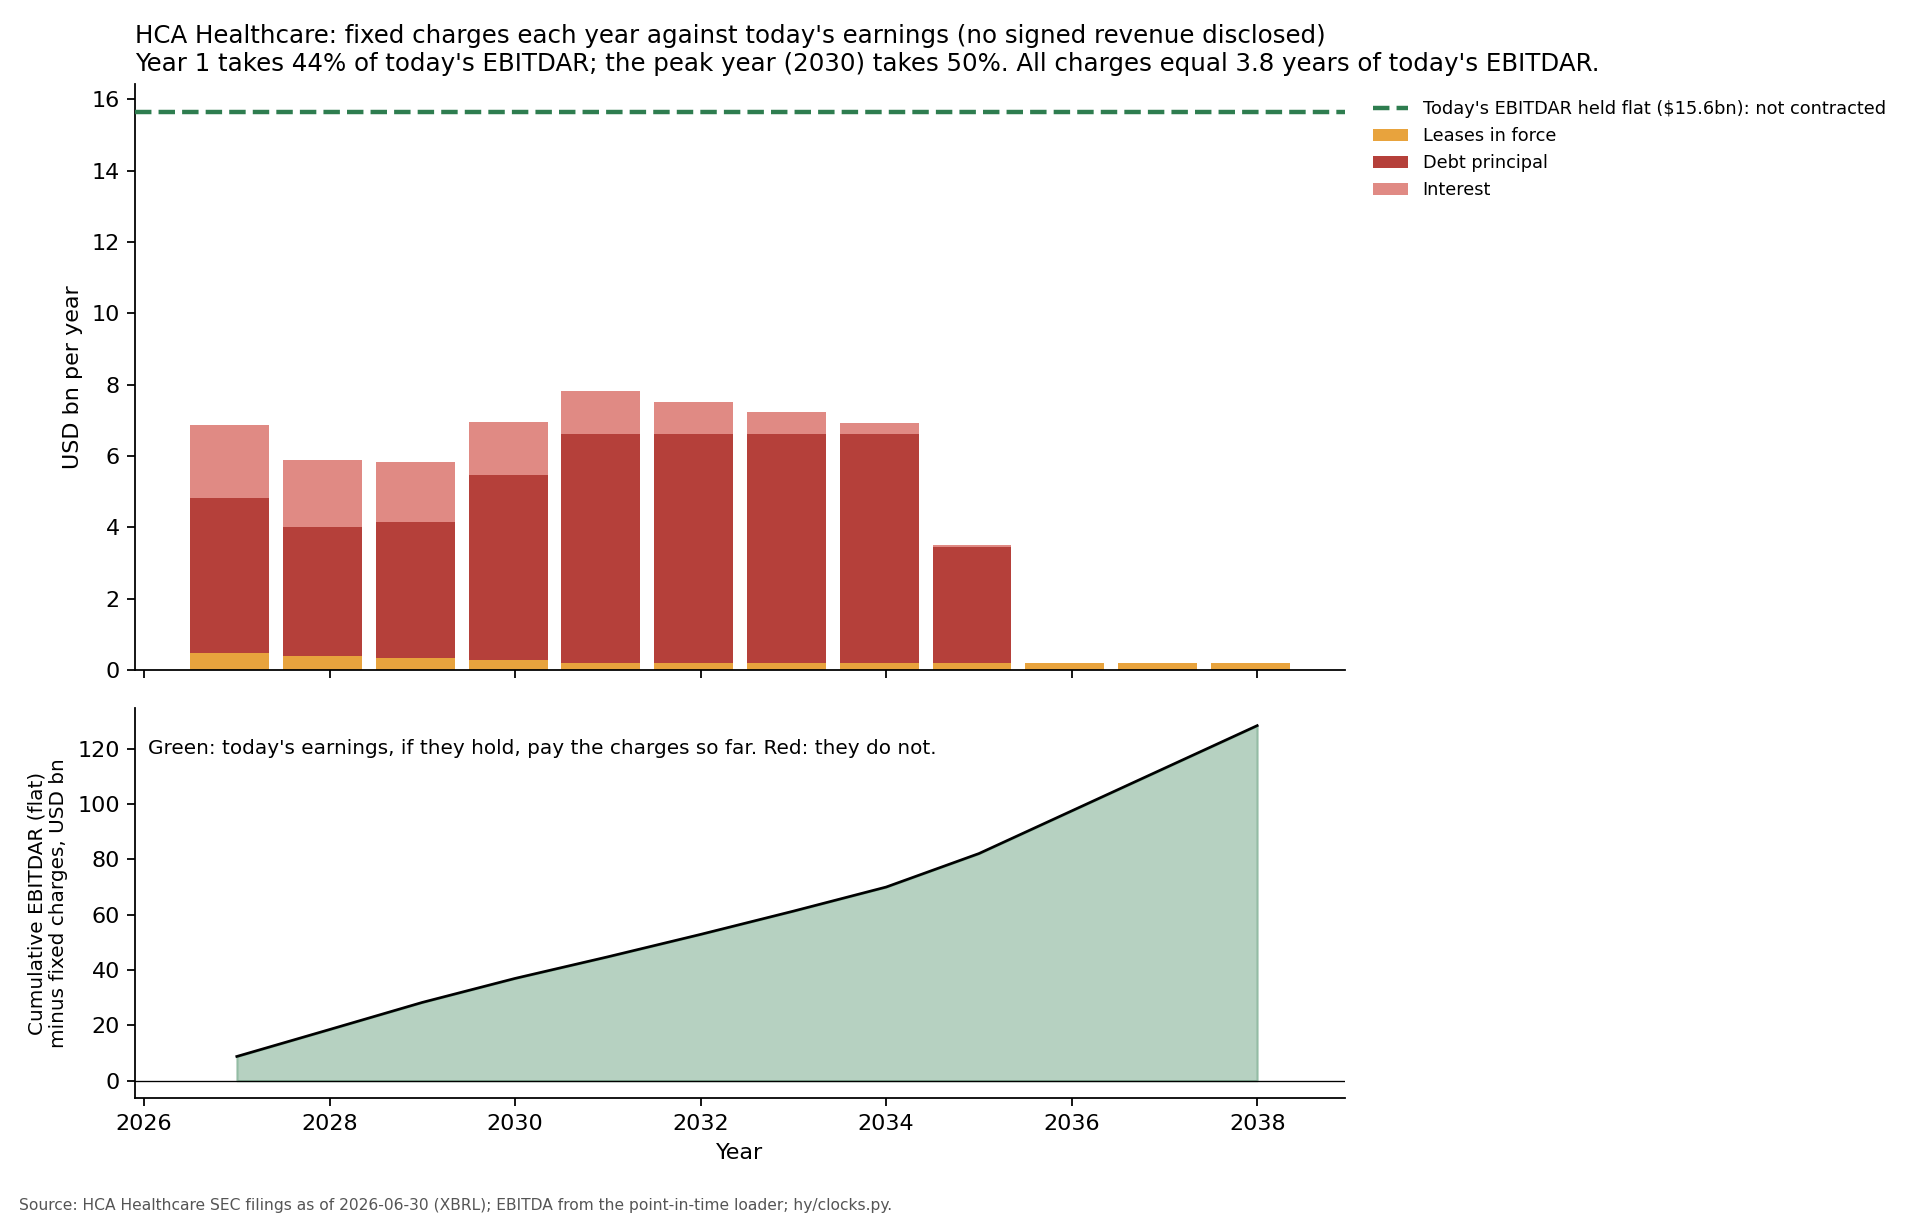
\includegraphics[width=0.95\linewidth]{figures/clocks_all_HCA.png}\caption*{The two clocks (section G2.1).}\end{figure}
\begin{figure}[H]\centering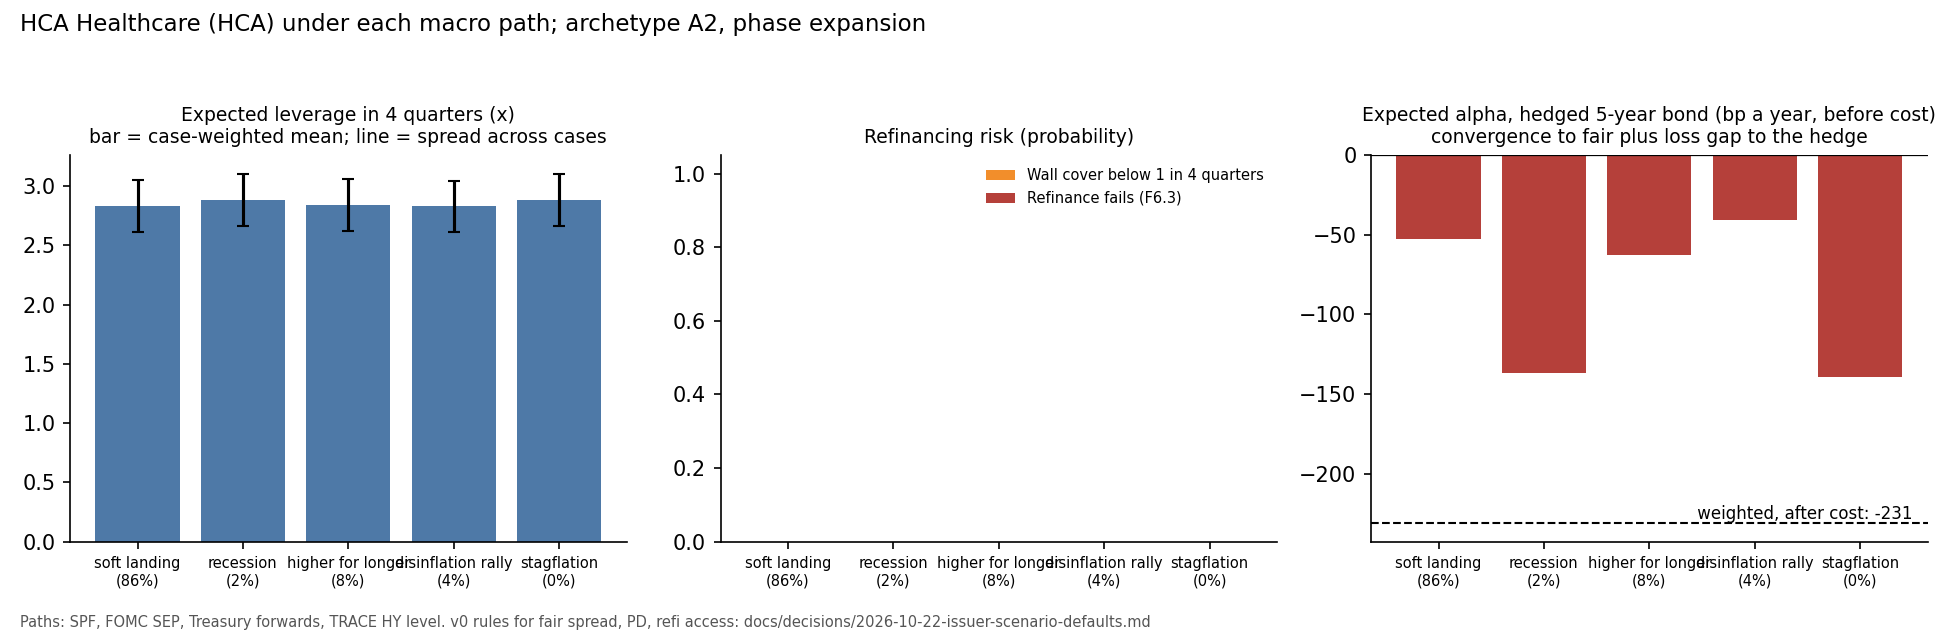
\includegraphics[width=0.95\linewidth]{figures/scenarios_HCA.png}\caption*{The company under each economic story (section G2.2).}\end{figure}
\begin{figure}[H]\centering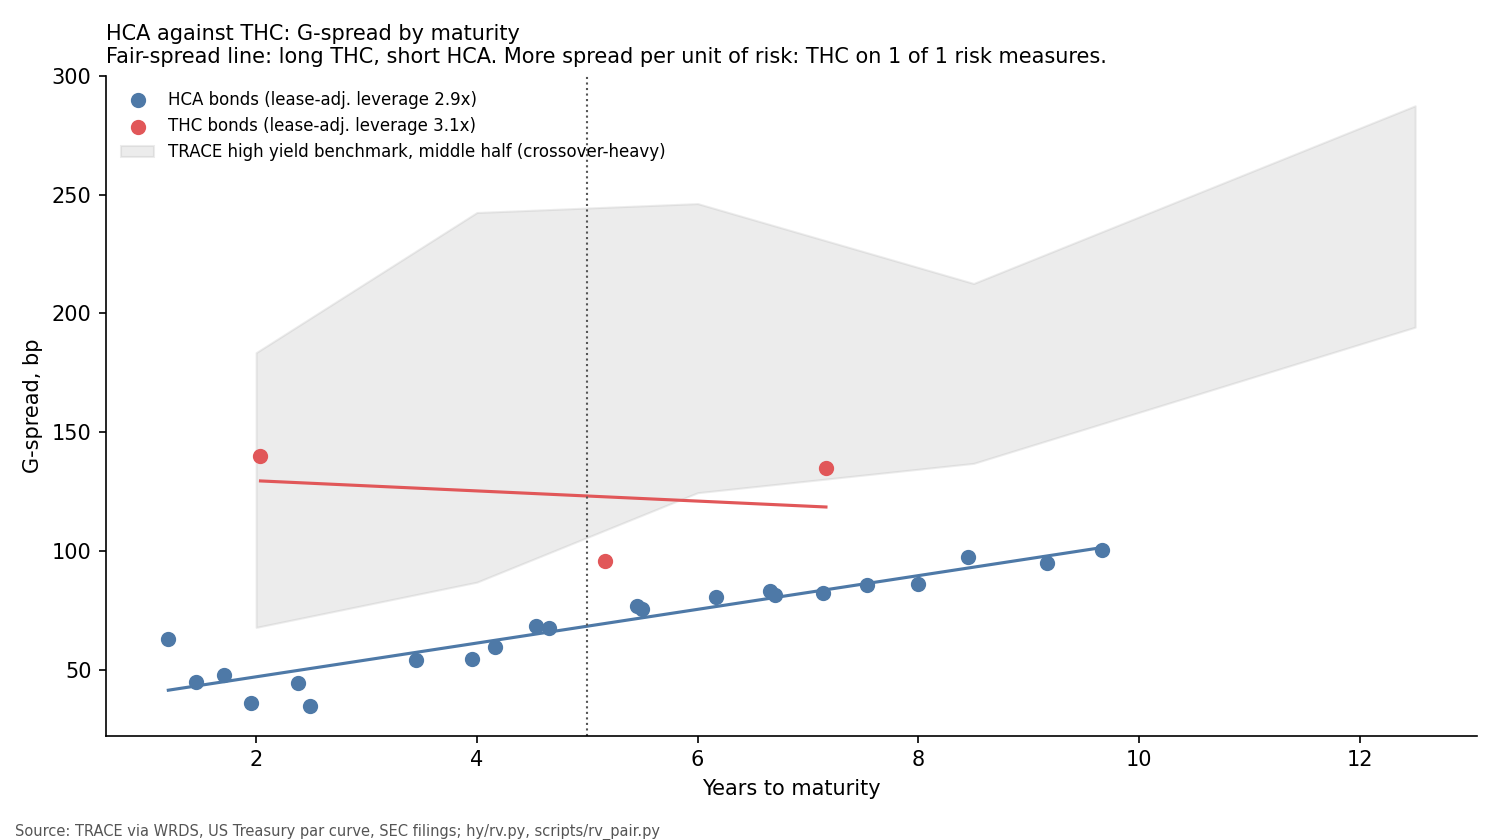
\includegraphics[width=0.85\linewidth]{figures/rv_HCA_THC.png}\caption*{The pair (section G2.3).}\end{figure}
\newpage
\section*{Tenet Healthcare (THC)}\pdfbookmark[1]{THC}{bm-THC}\label{memo-start-THC}
\par\noindent\fcolorbox{gray}{gray!6}{\parbox{\dimexpr\linewidth-2\fboxsep-2\fboxrule-1pt}{\sloppy \textbf{Recommendation.} Pass. This is a view of the company, not a trade: the expected profit does not beat trading costs. If the money went elsewhere, the best alternative in this run is NCLH. Position size and hedge: open until the call passes.}}

\subsection*{The combined view: four groups, one estimate}
Each group of methods estimates the same thing: what the bond should earn above a hedge, in bp a year. The combined estimate weighs the four groups. It ranks 2 of the issuers in this run. 4 of 5 groups point the same way as the combination.
\begin{center}\footnotesize\setlength{\tabcolsep}{3.5pt}\begin{tabular}{@{}lrrrl@{}}\toprule
Group & bp a year & Weight & Adds & Call \\\midrule
G1. Core process & +22 & 45\% & +10 & \textcolor{amber}{leans to owning} \\
G2 clocks. Two clocks & +183 & 20\% & +37 & \textcolor{good}{supports owning} \\
G2 rest. Built methods (rest) & +60 & 12\% & +7 & \textcolor{amber}{leans to owning} \\
G3. Credit skills & +0 & 12\% & +0 & \textcolor{good}{no objection} \\
G4. Books & +169 & 12\% & +20 & \textcolor{amber}{leans to owning} \\
\textbf{Combined, before trading costs} &  &  & \textbf{+73} &  \\
Trading costs &  &  & -174 &  \\
\textbf{Combined, after trading costs} &  &  & \textbf{-101} &  \\
Weighted cases and stories alone, after costs &  &  & -103 &  \\
Calibrated: after-cost number x measured slope 0.079 &  &  & -8 &  \\
\bottomrule\end{tabular}\end{center}
Against the weighted cases and stories alone, the combination is 2 bp a year higher: the other methods add to the case for owning the bond. A group that supports owning must beat the trading costs on its own. The weights are the user's choice: core process 45\%, two clocks 20\%, and 11.7\% each for the rest of the built methods, the credit skills and the books. The backtest alone would have put most weight on the built methods.
\par\noindent\fcolorbox{gray}{gray!6}{\parbox{\dimexpr\linewidth-2\fboxsep-2\fboxrule-1pt}{\sloppy \textbf{Alpha sizes are uncalibrated.} The backtest (2008 to 2026) shows that this kind of estimate ranks bonds well but overstates the size of the move. Realised alpha has been about 0.08 times the predicted alpha (standard error 0.05; 0.25 since 2019). The calibrated number multiplies by that slope: -8 bp a year after costs (-25 on the 2019 slope). The slope is not above zero by two standard errors, so the number ranks the bond but does not size it. Decision page: 2026-10-22-alpha-backtest-design. The backtest has no default-loss term yet.}}

\section*{G1. Core process: Gatto's steps, our method and rulebook, the relative value paper}
\par\noindent\fcolorbox{gray}{gray!6}{\parbox{\dimexpr\linewidth-2\fboxsep-2\fboxrule-1pt}{\sloppy \textbf{Verdict: \textcolor{amber}{leans to owning}.} This group reads Gatto's seven steps, our method and rulebook, and the relative value paper. Its estimate of expected profit is +22 bp a year before trading costs (costs are 174 bp a year); 2 of 4 of its weighted estimates point the same way. It carries 45\% of the combined view and ranks 5 of the issuers on this group alone. Best alternative for the same money: NCLH.}}
\begin{center}\footnotesize\setlength{\tabcolsep}{3.5pt}\begin{tabular}{@{}p{6.2cm}rrrp{4.2cm}@{}}\toprule
Estimate & bp a year & Weight in group & Adds & Where it comes from \\\midrule
Default chance the price assumes (shown, weight 0) & +20 & 0\% & +0 & F9; mapping C2 \\
Earnings quality, add-backs, FCF check (can only lower) & +0 & 25\% & +0 & F3; ebitda-addback-treatment; hy-model-standards \\
Access to new money and the funding gap & +96 & 25\% & +24 & F4; RV PDF E75-E76 \\
Debt against market value & -106 & 25\% & -27 & F7.7 \\
Return above cash, repriced in every story & +99 & 25\% & +25 & RV PDF E50-E60; C1, C3 \\
\bottomrule\end{tabular}\end{center}
\subsection*{G1.1 Thesis}
The bond pays 123 bp over Treasuries at 5 years. A company with its leverage (3.1x with leases) pays 93 bp on the fair line, so the bond is cheap by 30 bp. The bills outlast the signed contracts (section G2.1), so part of the extra spread pays for a renewal bet that the line does not see. What would reveal it, and when: open question.
\subsection*{G1.2 The business}
\begin{enumerate}
\item \textbf{What it sells:} Tenet Healthcare Corporation (“Tenet”) is a diversified healthcare services company with its headquarters in Dallas, Texas, and a Global Business Center (“GBC”) in the Philippines that supports various enterprise-wide administrative functions. We operate our expansive, nationwide care delivery network through direct and indirect subsidiaries, as well as downstream partnerships and joint ventures; the terms “we,” “our” and “us,” as used in this report and unless otherwise stated or indicated by t
\item \textbf{How it earns:} revenue 21.8bn a year at a 20\% EBITDA margin.
\item \textbf{What it must spend to stand still:} rent of about \$0.0bn a year, plus maintenance capital spending.
\item \textbf{Competition:} open question.
\item \textbf{What breaks it:} a reimbursement rule change, bad debt, or labour cost inflation.
\end{enumerate}
Business type: A2.
\subsection*{G1.3 Earnings, normalised}
Last 12 months: EBITDA \$4.3bn at a 20\% margin; margin trend over 8 quarters 1.4 (t-statistic: above 1 rising, below $-1$ falling). One-off items \$0.4bn. Free cash flow \$3.0bn: 71\% of EBITDA. Earnings-quality flags raised: EQ5 recurrence (of 4 tests the data supports). The add-back detail is in section G3.1.
\subsection*{G1.4 Cash, the funding gap, and the refinancing shock}
\begin{center}\footnotesize\setlength{\tabcolsep}{3.5pt}\begin{tabular}{@{}lr@{}}\toprule
Item & Value \\\midrule
Cash & \$2.2bn \\
Unused credit lines (tagged) & \$0.0bn \\
Less cash needed to run & \$0.1bn \\
Liquidity & \$2.1bn \\
Runway at today's cash burn, all capital spending (quarters) & no burn \\
First quarter cash runs out, severe case, maintenance spending only & no shortfall in 8 quarters \\
First quarter cash runs out, severe case, all committed spending & no shortfall in 8 quarters \\
\textbf{Runway we quote (the shortest)} & \textbf{none in 8 quarters} \\
Debt due in the next 18 months & \$0.1bn \\
Cash to meet debt due in a year, base case & 55.10x \\
Refinancing access score, likely story (0 to 6) & 3 \\
\bottomrule\end{tabular}\end{center}
\textbf{Funding gap if no lender refinances.} We add cash, the unused lines and the free cash flow of the cases, then take off the debt as it falls due, quarter by quarter. The minimum cash kept back is one month of cash operating costs (\$0.1bn).
\begin{center}\footnotesize\setlength{\tabcolsep}{3.5pt}\begin{tabular}{@{}lr@{}}\toprule
Measure & Value \\\midrule
Lowest point, likely story (maintenance spending only) & \$2.6bn \\
First quarter below zero, likely story & none in 8 quarters \\
Lowest point with all capital spending & \$2.6bn \\
First quarter below zero with all capital spending & none in 8 quarters \\
Lowest point, severe case & \$2.5bn \\
Severe case with all capital spending: first quarter below zero & no gap in 8 quarters \\
Lowest point, weighted over the stories & \$2.6bn \\
Debt due inside 8 quarters, share of all debt & 13\% \\
\bottomrule\end{tabular}\end{center}
\textbf{Refinancing shock.} \$1.7bn falls due in the next two years. It pays about 6.12\% today (TRACE coupons of bonds due inside 27 months). Refinanced at the forecast Treasury rate plus today's spread, yearly interest changes by \$0.0bn (0.1\% of EBITDA). Interest cover after refinancing: 5.1x; after capital spending 3.9x. Free cash flow after the shock: 22.8\% of debt.
\subsection*{G1.5 Debt: going-concern view}
\begin{center}\footnotesize\setlength{\tabcolsep}{3.5pt}\begin{tabular}{@{}lr@{}}\toprule
Measure & Value \\\midrule
Debt & \$13.2bn \\
Lease liabilities & \$0.0bn \\
EBITDA, last 12 months & \$4.3bn \\
Debt / EBITDA & 3.1x \\
(Debt + leases) / (EBITDA + rent) & 3.1x \\
Net debt / EBITDA & 2.6x \\
Coverage (after all capital spending) & 3.9x \\
Fixed-charge cover (after maintenance spending) & 4.16x \\
\bottomrule\end{tabular}\end{center}
\begin{center}\footnotesize\setlength{\tabcolsep}{3.5pt}\begin{tabular}{@{}lrrrrr@{}}\toprule
Bond & Coupon & Matures & Price & Yield & Spread (bp) \\\midrule
88033GDK3 & 6.12\% & 2028-10-01 & 100.1 & 6.07\% & 140 \\
88033GAV2 & 6.88\% & 2031-11-15 & 105.0 & 5.75\% & 96 \\
88033GDV9 & 6.00\% & 2033-11-15 & 98.8 & 6.21\% & 135 \\
\bottomrule\end{tabular}\end{center}
Claims view (who is paid what in a default): open question until the debt documents are read.
\subsection*{G1.6 Company value}
Market value of the whole company \$26bn (shares \$15bn plus net debt): 6.1x EBITDA; debt is 51\% of it. Our own valuation range and the bonds' recovery if the company defaults: open questions (they need a peer set and a distressed multiple).
\subsection*{G1.7 The decision against cash}
We put the same money in the bond nearest five years (88033GAV2, 6.88\% due 2031-11-15, price 104.98 plus 2.33 accrued) or in six-month Treasury bills at 4.20\%. In each story the bond either survives and is repriced, or defaults and returns 35 per 100 (a 40\% recovery paid a year later, valued at 15\% a year). In default the holder loses 68\% of the price paid.
\begin{center}\footnotesize\setlength{\tabcolsep}{3.5pt}\begin{tabular}{@{}lr@{}}\toprule
Measure & Value \\\midrule
Expected return above cash, bp a year & +99 \\
Chance of a loss over six months & 8.7\% \\
Chance of doing worse than cash & 9.0\% \\
Average loss in the worst 5\% of outcomes & 5.8\% \\
Same, with rates and the market hedged out, bp a year & +2 \\
Best alternative in this run (worst 5\% loss within the 25\% budget) & NCLH \\
Return given up against that alternative, bp a year & +348 \\
\bottomrule\end{tabular}\end{center}
\section*{G2. Built methods: two clocks, stories and cases, relative value, the gate}
\par\noindent\fcolorbox{gray}{gray!6}{\parbox{\dimexpr\linewidth-2\fboxsep-2\fboxrule-1pt}{\sloppy \textbf{Verdict: \textcolor{amber}{leans to owning}.} This group reads the spread level, the fair line and the pair, the economic stories, the health panel. Its estimate of expected profit is +60 bp a year before trading costs (costs are 174 bp a year); 4 of 5 of its weighted estimates point the same way. It carries 12\% of the combined view and ranks 3 of the issuers on this group alone. Gate: pass.}}
\begin{center}\footnotesize\setlength{\tabcolsep}{3.5pt}\begin{tabular}{@{}p{6.2cm}rrrp{4.2cm}@{}}\toprule
Estimate & bp a year & Weight in group & Adds & Where it comes from \\\midrule
Spread level: the extra pay over the market (carry) & -45 & 42\% & -19 & Spec S14 E0; K15 \\
Weighted cases and stories & +71 & 25\% & +18 & M5.4, M7.5 \\
Spread against the fair line & +72 & 17\% & +12 & M7.4, M7.5 \\
The pair & +428 & 8\% & +36 & M7.4; F10 S4 \\
Health panel & +158 & 8\% & +13 & F8 \\
\bottomrule\end{tabular}\end{center}
\subsection*{G2.1 The two clocks: bills against what pays for them}
\par\noindent\fcolorbox{gray}{gray!6}{\parbox{\dimexpr\linewidth-2\fboxsep-2\fboxrule-1pt}{\sloppy \textbf{Verdict: \textcolor{good}{supports owning}.} This group reads the bills the company owes against the revenue customers have signed for. Its estimate of expected profit is +183 bp a year before trading costs (costs are 174 bp a year); 1 of 1 of its weighted estimates point the same way. It carries 20\% of the combined view and ranks 2 of the issuers on this group alone. The clocks count as their own bucket in the combined view.}}
\begin{center}\footnotesize\setlength{\tabcolsep}{3.5pt}\begin{tabular}{@{}p{6.2cm}rrrp{4.2cm}@{}}\toprule
Estimate & bp a year & Weight in group & Adds & Where it comes from \\\midrule
The two clocks & +183 & 100\% & +183 & M4.7 \\
\bottomrule\end{tabular}\end{center}
Fixed bills total \$17.7bn, centred 3.3 years out: leases in force \$1.5bn, debt principal \$13.3bn, interest \$2.9bn. That is 4.2 years of today's EBITDAR; next year's bills take 46\% of it.
\begin{center}\footnotesize\setlength{\tabcolsep}{3.5pt}\begin{tabular}{@{}lr@{}}\toprule
Measure & Value \\\midrule
Signed contracts (RPO) & \$1.7bn \\
Where bills centre / where contract cash centres & year 3.3 / year 1.0 \\
Contracts 99\% booked by & year 2 \\
Margin needed for contracts to pay every bill & over 100\% (no margin is enough) \\
Company margin (EBITDAR) & 20\% \\
Share of bills paid by contracts at that margin & 2\% \\
Bills due after the contracts end & \$12.8bn (72\%) \\
\quad of which debt to refinance & \$11.8bn (66\%) \\
\quad of which rent and purchases to recontract & \$1.0bn (6\%) \\
Revenue to sign after the contracts end & 2.9 years of today's revenue \\
Largest running shortfall & \$17.4bn \\
Top three customers & n/a \\
Share paid by contracts at a 0.20 margin & 2\% \\
Share paid by contracts at a 0.35 margin & 3\% \\
Share paid by contracts at a 0.50 margin & 5\% \\
\bottomrule\end{tabular}\end{center}
\subsection*{G2.2 Economic stories and cases}
Cases on the most likely story (soft landing), stage of the cycle: expansion.
\begin{center}\scriptsize\setlength{\tabcolsep}{3.5pt}\begin{tabular}{@{}lrrrrrrr@{}}\toprule
Case & Weight & Growth / qtr & Leverage in 1 yr & Peak leverage & Lowest liquidity & Cash runs out & Refi fails \\\midrule
base & 64\% & 1.3\% & 2.9x & 3.1x & \$2.7bn & no & no \\
down moderate & 11\% & 0.4\% & 3.1x & 3.1x & \$2.7bn & no & no \\
down severe & 4\% & -0.1\% & 3.8x & 4.0x & \$2.6bn & no & no \\
upside & 21\% & 2.1\% & 2.7x & 3.0x & \$2.7bn & no & no \\
\bottomrule\end{tabular}\end{center}
\begin{center}\scriptsize\setlength{\tabcolsep}{3.5pt}\begin{tabular}{@{}lrrrrrr@{}}\toprule
Story & Chance & Leverage in 1 yr & Peak leverage (down) & Refi fails & Default chance & Expected profit (bp/yr) \\\midrule
soft landing & 86\% & 2.9x & 4.0x & 0\% & 0.7\% & 68 \\
recession & 2\% & 3.0x & 4.2x & 0\% & 1.7\% & 178 \\
higher for longer & 8\% & 2.9x & 4.0x & 0\% & 0.8\% & 81 \\
disinflation rally & 4\% & 2.9x & 4.0x & 0\% & 0.5\% & 52 \\
stagflation & 0\% & 3.0x & 4.2x & 0\% & 1.7\% & 181 \\
\bottomrule\end{tabular}\end{center}
\subsection*{G2.3 Relative value and the pair}
Fair line: log spread = -5.64 + 0.312 x leverage, fitted on 8 issuers in this run. 5-year spread 123 bp against a fair 93 bp.
\textbf{Against peers.} Peers are the high yield bonds that traded in 2026-08-31 (733 bonds with leverage on file), in the same 3 to 7 year maturity bucket. Sector: Health Care. Rating class: BB (implied by leverage). A positive value means the issuer pays more than the median peer.
\begin{center}\footnotesize\setlength{\tabcolsep}{3.5pt}\begin{tabular}{@{}lrr@{}}\toprule
Peer group & Excess spread to peers (ESP) & Spread per turn against peers (E13) \\\midrule
Sector and rating & -14\% & -6\% \\
Sector only & -74\% & -51\% \\
Rating only & -14\% & -6\% \\
\bottomrule\end{tabular}\end{center}
The sector and rating cell has fewer than five other issuers, so that row uses the rating cell.
\textbf{SPiDER} (spread per unit of debt to 10-year average EBITDA; Dynkin et al. 2021, ch. 14): cheaper than 41\% of the peer bonds across all sectors, and -26\% against sector and rating peers. It has no weight in the score: its edge beyond spread level is small (t 1.3 at 12 months).
\textbf{Against HCA.} Spreads at 5 years: HCA 68 bp, THC 123 bp.
\begin{center}\footnotesize\setlength{\tabcolsep}{3.5pt}\begin{tabular}{@{}lrrr@{}}\toprule
Spread per & HCA & THC & Cheaper \\\midrule
turn of leverage & 23 & 40 & THC \\
\bottomrule\end{tabular}\end{center}
The fair line favours long THC, short HCA: a gap of 51 bp, which halves in about 5 weeks on six months of trades. Under the stories the pair earns soft landing +120, recession +314, higher for longer +143, disinflation rally +93, stagflation +320 bp a year; weighted +125 bp before costs.
\subsection*{G2.4 Expected profit and price against our view}
Hedged 5-year bond over six months: 71 bp a year before trading costs, -103 bp after. It does not beat costs. The expected default loss is charged on the price paid: 68\% of it in default, not 60\% of face.
\begin{center}\footnotesize\setlength{\tabcolsep}{3.5pt}\begin{tabular}{@{}p{5.2cm}rrrrl@{}}\toprule
Question & Price assumes & Our view & Gap & Noise & Gap bigger than noise? \\\midrule
Default chance at the v0 price of risk (shown, not tested) & 1.0\% & 0.7\% & -0.3\% & open & not tested \\
Breakeven default probability, 12 months (loss on price) & 1.8\% & 0.7\% & -1.1\% & 0.9\% & yes \\
Leverage the spread is pricing & 4.00 & 3.11 & -0.88 & 0.90 & no \\
Spread against fair (bp) & 123 & 93 & -30 & 26 & yes \\
Rating class & open & BBB & open & open & not tested \\
Recovery if default (per 1 of face, discounted for delay) & open & 0.35 & open & open & not tested \\
\bottomrule\end{tabular}\end{center}
The first row turns the spread into a default chance with a fixed price of risk. That is not a real default chance, so it is shown but not tested. The breakeven row asks a cleaner question: is our default chance below the rate at which the spread only just pays for default losses?
\subsection*{G2.5 Risks and the health panel}
\begin{center}\footnotesize\setlength{\tabcolsep}{3.5pt}\begin{tabular}{@{}lrl@{}}\toprule
Measure & Value & Band \\\midrule
Refinancing access score (0 to 6) & 3.00 & \textcolor{amber}{amber} \\
Earnings-quality flags & 1.00 & \textcolor{amber}{amber} \\
Coverage & 3.92 & \textcolor{good}{green} \\
Fixed-charge cover & 4.16 & \textcolor{good}{green} \\
Cash conversion (FCF / EBITDA) & 0.71 & \textcolor{good}{green} \\
Free cash flow / debt & 0.23 & \textcolor{good}{green} \\
Cash to meet debt due in 1 year (base case) & 55.10 & \textcolor{good}{green} \\
Margin trend (t-statistic) & 1.35 & \textcolor{good}{green} \\
Weight on the downside cases & 0.15 & \textcolor{good}{green} \\
Chance debt due in 1 year is not covered & 0.00 & \textcolor{good}{green} \\
Chance cash runs out within 2 years & 0.00 & \textcolor{good}{green} \\
\bottomrule\end{tabular}\end{center}
\section*{G3. Credit skills: the lender's checklists applied to a public bond}
\par\noindent\fcolorbox{gray}{gray!6}{\parbox{\dimexpr\linewidth-2\fboxsep-2\fboxrule-1pt}{\sloppy \textbf{Verdict: \textcolor{good}{no objection}.} This group reads the lender's checklists: add-backs, covenants, watchlist, trend, memo structure. Its estimate of expected profit is +0 bp a year before trading costs (costs are 174 bp a year); 1 of 1 of its weighted estimates point the same way. It carries 12\% of the combined view and ranks 1 of the issuers on this group alone. Its estimates can only lower the combined number: a clean checklist earns no credit. Watchlist: none.}}
\begin{center}\footnotesize\setlength{\tabcolsep}{3.5pt}\begin{tabular}{@{}p{6.2cm}rrrp{4.2cm}@{}}\toprule
Estimate & bp a year & Weight in group & Adds & Where it comes from \\\midrule
Watchlist tier (can only lower) & +0 & 100\% & +0 & borrower-monitoring; covenant-compliance \\
\bottomrule\end{tabular}\end{center}
\subsection*{G3.1 Add-backs and their cash effect}
Reported EBITDA over the last 12 months is \$4.8bn. The company's own measure adds back \$-0.4bn of one-off items to reach \$4.3bn: -8.5\% of reported EBITDA (a negative figure is a one-off gain taken out). This is above the 5\% line the lender's checklist sets for one item. They do not recur in three quarters running. If every add-back were paid in cash, free cash flow would be \$3.0bn. The two roads to free cash flow (the EBITDA bridge, \$3.0bn; operating cash flow less capital spending, \$3.0bn) differ by 1\% of EBITDA: within the 10\% tolerance. The add-back table by category is an open question: the data has one total line.
\subsection*{G3.2 Covenant headroom}
The 10-Q and 10-K text state no maintenance test level. Public bonds are often tested only when the company borrows more or pays out cash. Headroom is an open question until the credit agreement is read.
\subsection*{G3.3 Watchlist and trajectory}
Watchlist tier: \textbf{none}: no trigger is met. EBITDA against the same months a year earlier: n/a (no plan is public, so last year stands in for it).
\begin{center}\footnotesize\setlength{\tabcolsep}{3.5pt}\begin{tabular}{@{}llll@{}}\toprule
Measure & Direction & How much weight & Change on a year earlier, last quarter \\\midrule
revenue & improving & trend & 6.8\% \\
EBITDA & open & no data & n/a \\
EBITDA margin & open & no data & n/a \\
cash conversion & open & no data & n/a \\
\bottomrule\end{tabular}\end{center}
One quarter is an observation, two a data point, three or four a trend.
\subsection*{G3.4 Memo structure check}
\begin{center}\footnotesize\setlength{\tabcolsep}{3.5pt}\begin{tabular}{@{}lp{9cm}l@{}}\toprule
Section & Requires & Status \\\midrule
Executive summary & the business in one sentence, the opportunity, 2 to 3 reasons, 2 to 3 risks & \textcolor{good}{pass} \\
Capital structure & each tranche with face, coupon, maturity; senior, total and net leverage; LTV & \textcolor{amber}{open} \\
Terms & maintenance covenant levels and test dates; incurrence baskets; call terms & \textcolor{amber}{open} \\
Investment merits & free cash flow generation and the base-case deleveraging path & \textcolor{good}{pass} \\
Key risks & 3 to 5 issuer-specific risks, each with a mitigant & \textcolor{amber}{open} \\
Historical financials & at least 3 years, quarterly where available & \textcolor{good}{pass} \\
EBITDA adjustments & reported-to-adjusted bridge with the load as a share of EBITDA and the 5\% flag & \textcolor{amber}{open} \\
Model output & base and downside: EBITDA, FCF, leverage path, covenant headroom, liquidity runway & \textcolor{amber}{open} \\
\bottomrule\end{tabular}\end{center}
\textbf{Rules that do not transfer to a public bond:}\begin{itemize}\item The compliance certificate is the source of truth; public bonds have none. Headroom here uses our own ratio against a level parsed from the filing text. (covenant-compliance)\item Equity cures, step-down schedules and window-dressing checks need the credit agreement and monthly revolver balances. (covenant-compliance)\item Performance against the sponsor plan: no plan is public. The proxy is the same quarters a year earlier. (borrower-monitoring)\item Add-back caps and the certificate reconciliation live in the credit agreement. Compustat gives one special-items line, not the category table. (ebitda-addback-treatment)\item Sources and uses at entry, the sponsor case and the management call apply to new loans, not to bonds bought in the secondary market. (credit-memo-standards)\item Monthly lender packages do not exist for public issuers; XBRL quarters replace them. (quarterly-package-extraction)\end{itemize}
\section*{G4. Books: Kricheff, and Ganguin and Bilardello (S\&P)}
\par\noindent\fcolorbox{gray}{gray!6}{\parbox{\dimexpr\linewidth-2\fboxsep-2\fboxrule-1pt}{\sloppy \textbf{Verdict: \textcolor{amber}{leans to owning}.} This group reads Kricheff's cash bridge and ratios; the S\&P risk profiles and rating anchor. Its estimate of expected profit is +169 bp a year before trading costs (costs are 174 bp a year); 2 of 2 of its weighted estimates point the same way. It carries 12\% of the combined view and ranks 1 of the issuers on this group alone. S\&P anchor class: BBB.}}
\begin{center}\footnotesize\setlength{\tabcolsep}{3.5pt}\begin{tabular}{@{}p{6.2cm}rrrp{4.2cm}@{}}\toprule
Estimate & bp a year & Weight in group & Adds & Where it comes from \\\midrule
Spread against the S\&P risk score & +133 & 50\% & +66 & Ganguin and Bilardello ch. 10 \\
Spread per turn of leverage (with the trap guard) & +205 & 50\% & +102 & Kricheff ch. 21 \\
\bottomrule\end{tabular}\end{center}
\subsection*{G4.1 Kricheff's cash-flow bridge and ratio set}
\begin{center}\footnotesize\setlength{\tabcolsep}{3.5pt}\begin{tabular}{@{}lr@{}}\toprule
Line (last 12 months) & Value \\\midrule
Adjusted EBITDA & \$4.3bn \\
less capital spending & \$1.0bn \\
less cash interest & \$0.8bn \\
less cash taxes & \$0.5bn \\
less increase in working capital & \$-1.1bn \\
\textbf{Free cash flow} & \textbf{\$3.0bn} \\
Check: free cash flow before capital spending less operating cash flow & \$-0.0bn \\
Free cash flow after dividends & open (dividends not loaded) \\
\bottomrule\end{tabular}\end{center}
\begin{center}\footnotesize\setlength{\tabcolsep}{3.5pt}\begin{tabular}{@{}lrlr@{}}\toprule
Ratio & Value & Ratio & Value \\\midrule
EBITDA / cash interest & 5.1x & Debt / EBITDA & 3.1x \\
(EBITDA $-$ capex) / interest & 3.9x & Net debt / EBITDA & 2.6x \\
(EBITDA $-$ maintenance capex) / interest & 4.2x & Free cash flow / debt & 23.0\% \\
EBITDA / debt (highest rate at 1x cover) & 32.0\% & Market value / EBITDA & 6.2x \\
Equity cushion (1 $-$ debt / market value) & 49\% & Spread per turn of leverage & 40 bp \\
\bottomrule\end{tabular}\end{center}
Kricheff's snapshot rule: operating cash flow covers capital spending. Spread per turn compares the bond with the run's median of 38 bp a turn. Kricheff warns that a high spread per turn can mean weak cash flow, not value; read it with free cash flow / debt. The book measures leverage through each bond's rank; with no face by rank, total leverage stands in.
\subsection*{G4.2 The S\&P risk profiles and the rating anchor}
S\&P adds leases to debt and scores each ratio against the median of each rating class (CreditStats 2002, from the book). Scores run from 1 (safest) to 10 (default).
\begin{center}\footnotesize\setlength{\tabcolsep}{3.5pt}\begin{tabular}{@{}lrrrr@{}}\toprule
Ratio & Value & Score & BB median & B median \\\midrule
Debt / (debt + market value of equity) & 47\% & 5.6 & 57.5\% & 78.5\% \\
Funds from operations / debt & 22\% & 7.1 & 19.5\% & 10.8\% \\
Free operating cash flow / debt & 23\% & 3.6 & 8.5\% & 2.5\% \\
EBITDA / interest (with lease interest) & 5.1x & 5.8 & 3.2x & 1.8x \\
EBITDA margin & 20\% & 5.0 &  &  \\
\bottomrule\end{tabular}\end{center}
Financial risk score 5.5. Business risk score 4.0: industry 4, steadiness of sales 3 (year-on-year growth varies by 4.8\%), customer spread 5. The book puts 55\% of the weight on business risk for this class, so the default risk score is 4.7: the \textbf{BBB} class. The line from score to spread across the run did not slope upward, so it gives no estimate. The 2005 edition has no modern anchor table; its own weighting table stands in for it.
\section*{Coming events, open questions, and the record}
\begin{itemize}\item Next quarterly results (estimated from filing cadence): 2026-10-28 (estimate).\item Debt due by 1.0 years out:  - \$0.1bn.\end{itemize}
\textbf{Open questions, most important first:}\begin{enumerate}\item A dated catalyst that would close the gap (G2).\item The observable and level that would prove the call wrong (G8).\item Face amount of each tranche and the secured debt ahead of the bonds (debt note table).\item Claims view: allowed claims by class and the entity map (framework F5).\item Maintenance covenant levels: none stated in the 10-Q or 10-K text; read the credit agreement exhibit (public bonds are often incurrence-only).\item Revolver commitment, draw, and borrowing base: not tagged; read the credit agreement note.\item F4 points 3 (unencumbered assets) and 6 (sponsor support) are scored 0 until read.\item Recovery, delay and the required return on a defaulted claim are v0 (R = 0.4, tau = 1 year, k = 15\%); the claims view and documents replace them.\item Peer set of at least four issuers of the same archetype (F3.3) for the valuation range (F7.1).\item Distressed multiple (F7.3) and the recovery of the bonds if the company defaults (F7.9).\end{enumerate}
\textbf{Record (filled at exit):} exit date; return against the rating-matched index; worst point against the index; reason; the rule that would have helped.
\newpage
\begin{figure}[H]\centering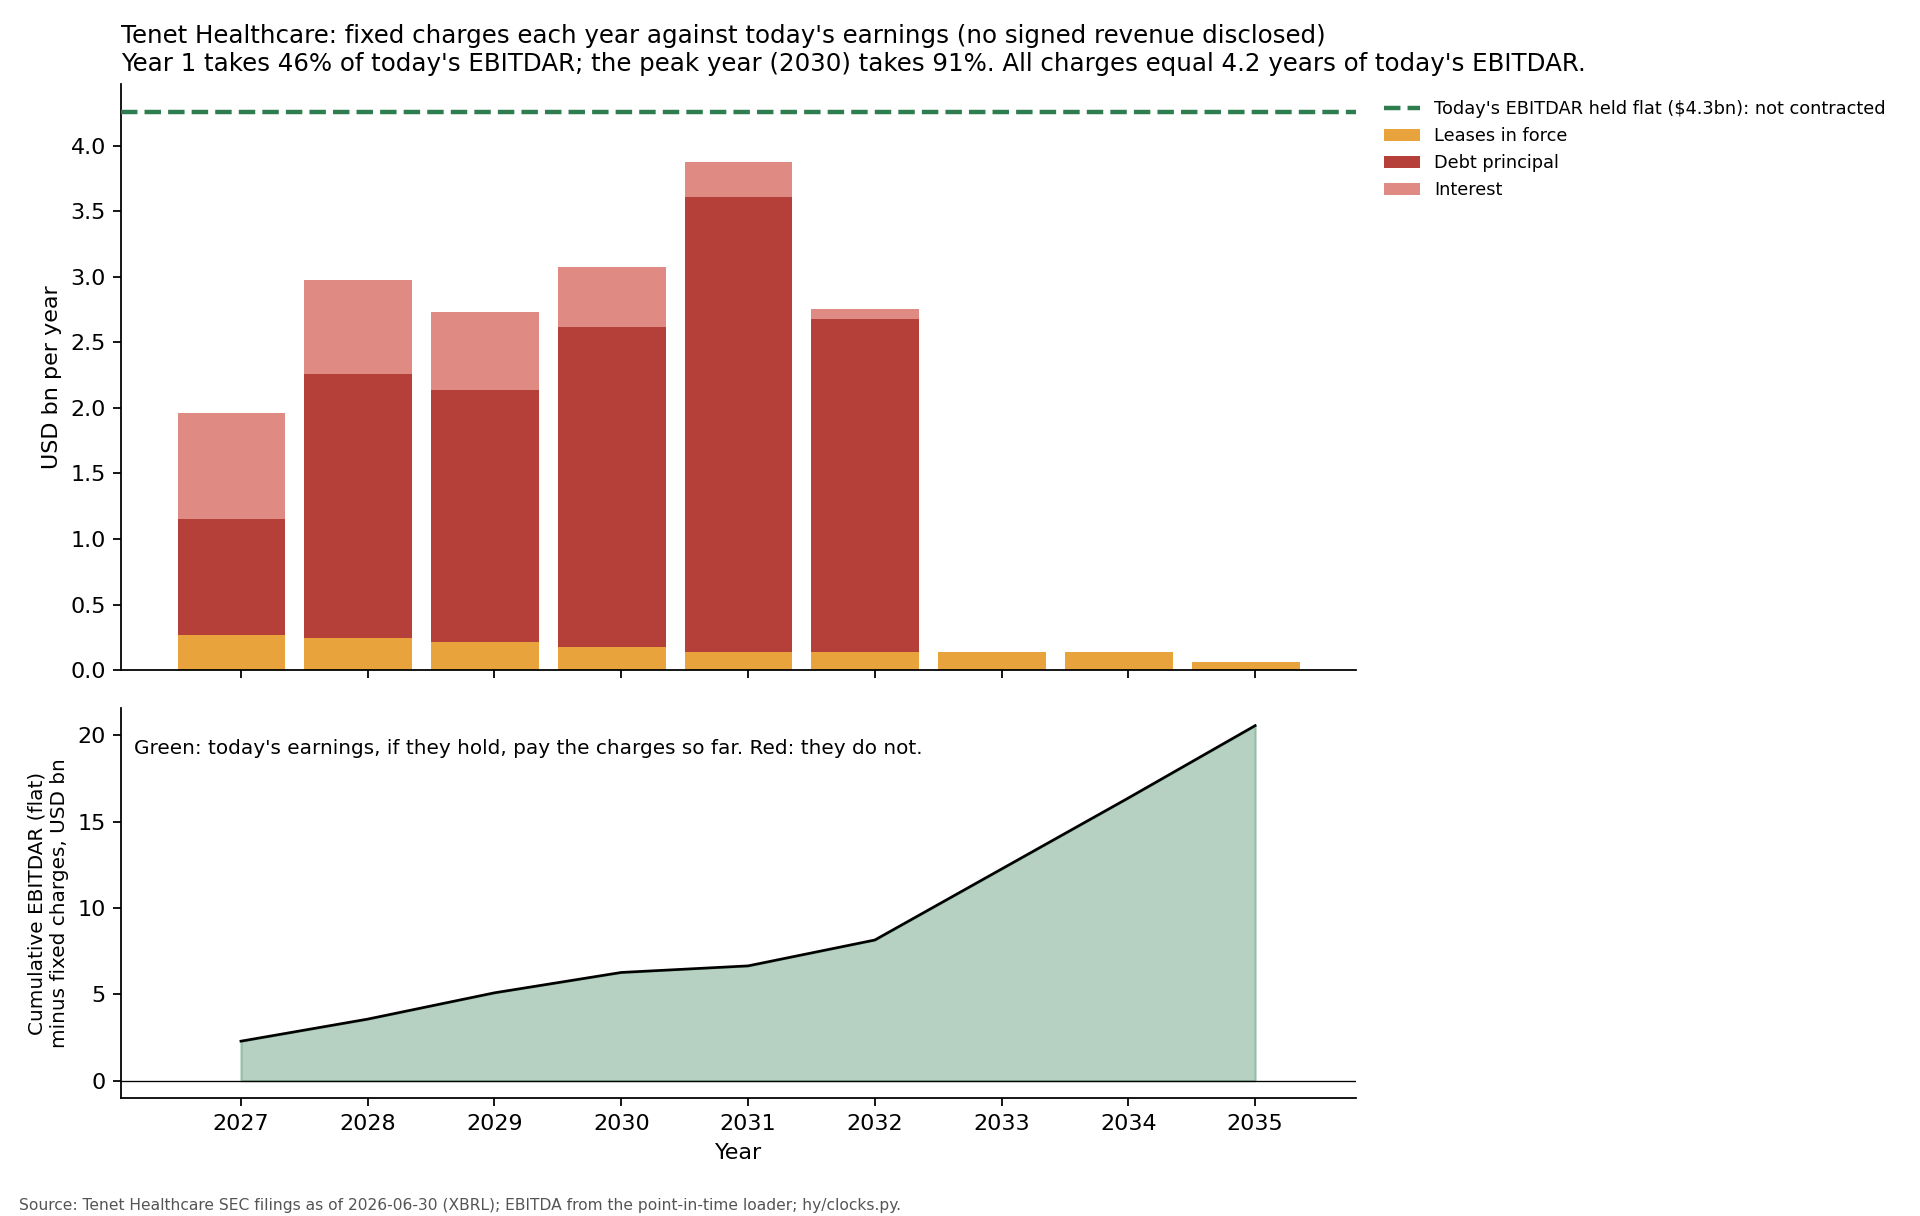
\includegraphics[width=0.95\linewidth]{figures/clocks_all_THC.png}\caption*{The two clocks (section G2.1).}\end{figure}
\begin{figure}[H]\centering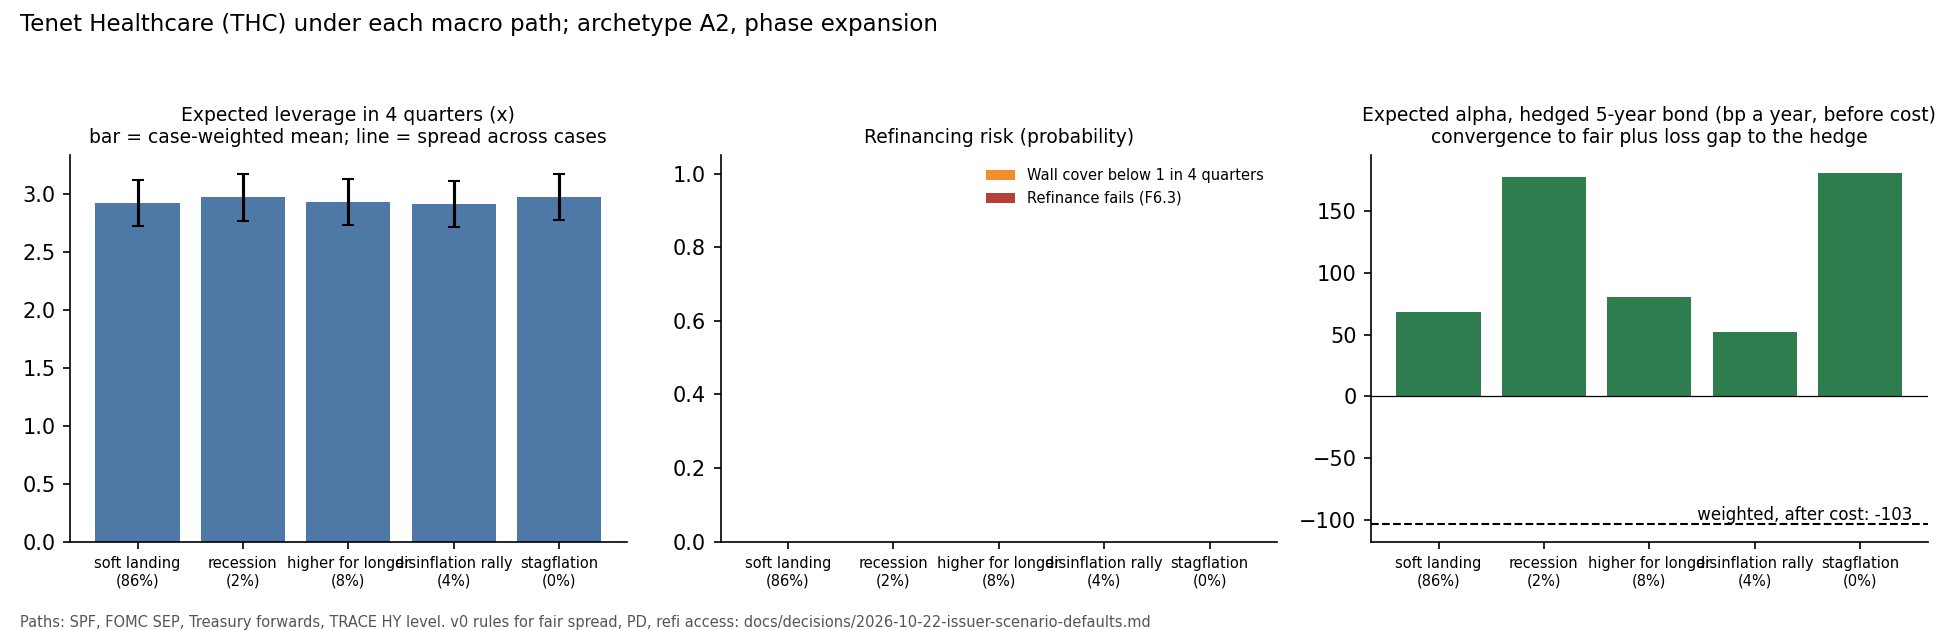
\includegraphics[width=0.95\linewidth]{figures/scenarios_THC.png}\caption*{The company under each economic story (section G2.2).}\end{figure}
\begin{figure}[H]\centering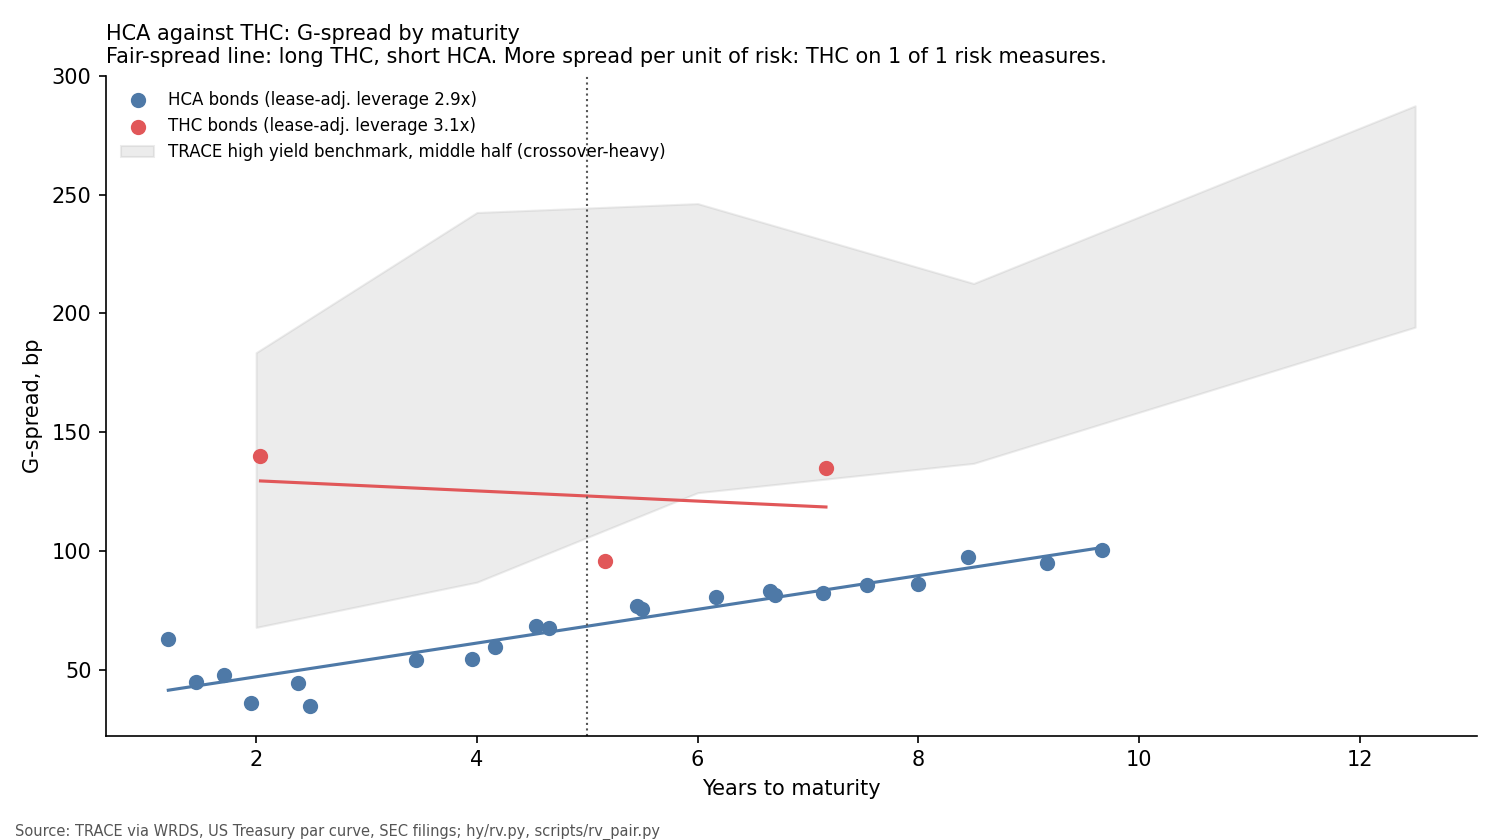
\includegraphics[width=0.85\linewidth]{figures/rv_HCA_THC.png}\caption*{The pair (section G2.3).}\end{figure}
\newpage
\section*{Carnival Corp (CCL)}\pdfbookmark[1]{CCL}{bm-CCL}\label{memo-start-CCL}
\par\noindent\fcolorbox{gray}{gray!6}{\parbox{\dimexpr\linewidth-2\fboxsep-2\fboxrule-1pt}{\sloppy \textbf{Recommendation.} Pass. This is a view of the company, not a trade: the expected profit does not beat trading costs. If the money went elsewhere, the best alternative in this run is NCLH. Position size and hedge: open until the call passes.}}

\subsection*{The combined view: four groups, one estimate}
Each group of methods estimates the same thing: what the bond should earn above a hedge, in bp a year. The combined estimate weighs the four groups. It ranks 3 of the issuers in this run. 4 of 5 groups point the same way as the combination.
\begin{center}\footnotesize\setlength{\tabcolsep}{3.5pt}\begin{tabular}{@{}lrrrl@{}}\toprule
Group & bp a year & Weight & Adds & Call \\\midrule
G1. Core process & +72 & 45\% & +32 & \textcolor{amber}{leans to owning} \\
G2 clocks. Two clocks & +88 & 20\% & +18 & \textcolor{amber}{leans to owning} \\
G2 rest. Built methods (rest) & +16 & 12\% & +2 & \textcolor{amber}{leans to owning} \\
G3. Credit skills & +0 & 12\% & +0 & \textcolor{good}{no objection} \\
G4. Books & +100 & 12\% & +12 & \textcolor{amber}{leans to owning} \\
\textbf{Combined, before trading costs} &  &  & \textbf{+63} &  \\
Trading costs &  &  & -174 &  \\
\textbf{Combined, after trading costs} &  &  & \textbf{-110} &  \\
Weighted cases and stories alone, after costs &  &  & -116 &  \\
Calibrated: after-cost number x measured slope 0.079 &  &  & -9 &  \\
\bottomrule\end{tabular}\end{center}
Against the weighted cases and stories alone, the combination is 6 bp a year higher: the other methods add to the case for owning the bond. A group that supports owning must beat the trading costs on its own. The weights are the user's choice: core process 45\%, two clocks 20\%, and 11.7\% each for the rest of the built methods, the credit skills and the books. The backtest alone would have put most weight on the built methods.
\par\noindent\fcolorbox{gray}{gray!6}{\parbox{\dimexpr\linewidth-2\fboxsep-2\fboxrule-1pt}{\sloppy \textbf{Alpha sizes are uncalibrated.} The backtest (2008 to 2026) shows that this kind of estimate ranks bonds well but overstates the size of the move. Realised alpha has been about 0.08 times the predicted alpha (standard error 0.05; 0.25 since 2019). The calibrated number multiplies by that slope: -9 bp a year after costs (-28 on the 2019 slope). The slope is not above zero by two standard errors, so the number ranks the bond but does not size it. Decision page: 2026-10-22-alpha-backtest-design. The backtest has no default-loss term yet.}}

\section*{G1. Core process: Gatto's steps, our method and rulebook, the relative value paper}
\par\noindent\fcolorbox{gray}{gray!6}{\parbox{\dimexpr\linewidth-2\fboxsep-2\fboxrule-1pt}{\sloppy \textbf{Verdict: \textcolor{amber}{leans to owning}.} This group reads Gatto's seven steps, our method and rulebook, and the relative value paper. Its estimate of expected profit is +72 bp a year before trading costs (costs are 174 bp a year); 3 of 4 of its weighted estimates point the same way. It carries 45\% of the combined view and ranks 3 of the issuers on this group alone. Best alternative for the same money: NCLH.}}
\begin{center}\footnotesize\setlength{\tabcolsep}{3.5pt}\begin{tabular}{@{}p{6.2cm}rrrp{4.2cm}@{}}\toprule
Estimate & bp a year & Weight in group & Adds & Where it comes from \\\midrule
Default chance the price assumes (shown, weight 0) & +20 & 0\% & +0 & F9; mapping C2 \\
Earnings quality, add-backs, FCF check (can only lower) & +0 & 25\% & +0 & F3; ebitda-addback-treatment; hy-model-standards \\
Access to new money and the funding gap & +96 & 25\% & +24 & F4; RV PDF E75-E76 \\
Debt against market value & +38 & 25\% & +9 & F7.7 \\
Return above cash, repriced in every story & +154 & 25\% & +38 & RV PDF E50-E60; C1, C3 \\
\bottomrule\end{tabular}\end{center}
\subsection*{G1.1 Thesis}
The bond pays 129 bp over Treasuries at 5 years. A company with its leverage (3.5x with leases) pays 105 bp on the fair line, so the bond is cheap by 24 bp. What would reveal it, and when: open question.
\subsection*{G1.2 The business}
\begin{enumerate}
\item \textbf{What it sells:} A. Overview I.Summary Carnival Corporation was incorporated in Panama in 1974 and Carnival plc was incorporated in England and Wales in 2000.
\item \textbf{How it earns:} revenue 27.3bn a year at a 27\% EBITDA margin.
\item \textbf{What it must spend to stand still:} rent of about \$0.0bn a year, plus maintenance capital spending.
\item \textbf{Competition:} open question.
\item \textbf{What breaks it:} contracts roll off or churn; the asset value cycle turns.
\end{enumerate}
Business type: A5.
\subsection*{G1.3 Earnings, normalised}
Last 12 months: EBITDA \$7.3bn at a 27\% margin; margin trend over 8 quarters -0.7 (t-statistic: above 1 rising, below $-1$ falling). One-off items \$-0.1bn. Free cash flow \$3.2bn: 44\% of EBITDA. Earnings-quality flags raised: EQ5 recurrence (of 4 tests the data supports). The add-back detail is in section G3.1.
\subsection*{G1.4 Cash, the funding gap, and the refinancing shock}
\begin{center}\footnotesize\setlength{\tabcolsep}{3.5pt}\begin{tabular}{@{}lr@{}}\toprule
Item & Value \\\midrule
Cash & \$2.2bn \\
Unused credit lines (tagged) & \$0.0bn \\
Less cash needed to run & \$0.1bn \\
Liquidity & \$2.1bn \\
Runway at today's cash burn, all capital spending (quarters) & no burn \\
First quarter cash runs out, severe case, maintenance spending only & no shortfall in 8 quarters \\
First quarter cash runs out, severe case, all committed spending & no shortfall in 8 quarters \\
\textbf{Runway we quote (the shortest)} & \textbf{none in 8 quarters} \\
Debt due in the next 18 months & \$3.3bn \\
Cash to meet debt due in a year, base case & 6.49x \\
Refinancing access score, likely story (0 to 6) & 3 \\
\bottomrule\end{tabular}\end{center}
\textbf{Funding gap if no lender refinances.} We add cash, the unused lines and the free cash flow of the cases, then take off the debt as it falls due, quarter by quarter. The minimum cash kept back is one month of cash operating costs (\$1.7bn).
\begin{center}\footnotesize\setlength{\tabcolsep}{3.5pt}\begin{tabular}{@{}lr@{}}\toprule
Measure & Value \\\midrule
Lowest point, likely story (maintenance spending only) & \$1.1bn \\
First quarter below zero, likely story & none in 8 quarters \\
Lowest point with all capital spending & \$0.4bn \\
First quarter below zero with all capital spending & none in 8 quarters \\
Lowest point, severe case & \$-1.5bn \\
Severe case with all capital spending: first quarter below zero & quarter 2 \\
Lowest point, weighted over the stories & \$1.1bn \\
Debt due inside 8 quarters, share of all debt & 13\% \\
\bottomrule\end{tabular}\end{center}
\textbf{Refinancing shock.} \$3.3bn falls due in the next two years. It pays about 6.65\% today (TRACE coupons of bonds due inside 27 months). Refinanced at the forecast Treasury rate plus today's spread, yearly interest changes by \$-0.0bn (-0.1\% of EBITDA). Interest cover after refinancing: 6.1x; after capital spending 3.1x. Free cash flow after the shock: 12.6\% of debt.
\subsection*{G1.5 Debt: going-concern view}
\begin{center}\footnotesize\setlength{\tabcolsep}{3.5pt}\begin{tabular}{@{}lr@{}}\toprule
Measure & Value \\\midrule
Debt & \$25.6bn \\
Lease liabilities & \$0.0bn \\
EBITDA, last 12 months & \$7.3bn \\
Debt / EBITDA & 3.5x \\
(Debt + leases) / (EBITDA + rent) & 3.5x \\
Net debt / EBITDA & 3.2x \\
Coverage (after all capital spending) & 3.1x \\
Fixed-charge cover (after maintenance spending) & 3.86x \\
\bottomrule\end{tabular}\end{center}
\begin{center}\footnotesize\setlength{\tabcolsep}{3.5pt}\begin{tabular}{@{}lrrrrr@{}}\toprule
Bond & Coupon & Matures & Price & Yield & Spread (bp) \\\midrule
143658AH5 & 6.65\% & 2028-01-15 & 101.9 & 5.15\% & 66 \\
143658CB6 & 5.12\% & 2029-05-01 & 98.7 & 5.68\% & 96 \\
143658BY7 & 5.75\% & 2030-03-15 & 99.6 & 5.87\% & 111 \\
143658BZ4 & 5.87\% & 2031-06-15 & 99.1 & 6.09\% & 131 \\
143658CA8 & 5.75\% & 2032-08-01 & 98.0 & 6.16\% & 134 \\
143658BX9 & 6.12\% & 2033-02-15 & 98.9 & 6.34\% & 151 \\
\bottomrule\end{tabular}\end{center}
Claims view (who is paid what in a default): open question until the debt documents are read.
\subsection*{G1.6 Company value}
Market value of the whole company \$62bn (shares \$38bn plus net debt): 8.4x EBITDA; debt is 41\% of it. Our own valuation range and the bonds' recovery if the company defaults: open questions (they need a peer set and a distressed multiple).
\subsection*{G1.7 The decision against cash}
We put the same money in the bond nearest five years (143658BZ4, 5.88\% due 2031-06-15, price 99.11 plus 1.52 accrued) or in six-month Treasury bills at 4.20\%. In each story the bond either survives and is repriced, or defaults and returns 35 per 100 (a 40\% recovery paid a year later, valued at 15\% a year). In default the holder loses 65\% of the price paid.
\begin{center}\footnotesize\setlength{\tabcolsep}{3.5pt}\begin{tabular}{@{}lr@{}}\toprule
Measure & Value \\\midrule
Expected return above cash, bp a year & +154 \\
Chance of a loss over six months & 8.7\% \\
Chance of doing worse than cash & 9.1\% \\
Average loss in the worst 5\% of outcomes & 5.9\% \\
Same, with rates and the market hedged out, bp a year & +24 \\
Best alternative in this run (worst 5\% loss within the 25\% budget) & NCLH \\
Return given up against that alternative, bp a year & +292 \\
\bottomrule\end{tabular}\end{center}
\section*{G2. Built methods: two clocks, stories and cases, relative value, the gate}
\par\noindent\fcolorbox{gray}{gray!6}{\parbox{\dimexpr\linewidth-2\fboxsep-2\fboxrule-1pt}{\sloppy \textbf{Verdict: \textcolor{amber}{leans to owning}.} This group reads the spread level, the fair line and the pair, the economic stories, the health panel. Its estimate of expected profit is +16 bp a year before trading costs (costs are 174 bp a year); 3 of 5 of its weighted estimates point the same way. It carries 12\% of the combined view and ranks 4 of the issuers on this group alone. Gate: pass.}}
\begin{center}\footnotesize\setlength{\tabcolsep}{3.5pt}\begin{tabular}{@{}p{6.2cm}rrrp{4.2cm}@{}}\toprule
Estimate & bp a year & Weight in group & Adds & Where it comes from \\\midrule
Spread level: the extra pay over the market (carry) & -39 & 42\% & -16 & Spec S14 E0; K15 \\
Weighted cases and stories & +57 & 25\% & +14 & M5.4, M7.5 \\
Spread against the fair line & +58 & 17\% & +10 & M7.4, M7.5 \\
The pair & -22 & 8\% & -2 & M7.4; F10 S4 \\
Health panel & +117 & 8\% & +10 & F8 \\
\bottomrule\end{tabular}\end{center}
\subsection*{G2.1 The two clocks: bills against what pays for them}
\par\noindent\fcolorbox{gray}{gray!6}{\parbox{\dimexpr\linewidth-2\fboxsep-2\fboxrule-1pt}{\sloppy \textbf{Verdict: \textcolor{amber}{leans to owning}.} This group reads the bills the company owes against the revenue customers have signed for. Its estimate of expected profit is +88 bp a year before trading costs (costs are 174 bp a year); 1 of 1 of its weighted estimates point the same way. It carries 20\% of the combined view and ranks 4 of the issuers on this group alone. The clocks count as their own bucket in the combined view.}}
\begin{center}\footnotesize\setlength{\tabcolsep}{3.5pt}\begin{tabular}{@{}p{6.2cm}rrrp{4.2cm}@{}}\toprule
Estimate & bp a year & Weight in group & Adds & Where it comes from \\\midrule
The two clocks & +88 & 100\% & +88 & M4.7 \\
\bottomrule\end{tabular}\end{center}
Fixed bills total \$50.7bn, centred 4.7 years out: leases in force \$1.8bn, debt principal \$25.6bn, interest \$4.8bn, purchase commitments \$18.5bn. That is 6.9 years of today's EBITDAR; next year's bills take 63\% of it.
The company discloses no material signed revenue, so the second clock is today's earnings held flat (chart at the end).
\subsection*{G2.2 Economic stories and cases}
Cases on the most likely story (soft landing), stage of the cycle: expansion.
\begin{center}\scriptsize\setlength{\tabcolsep}{3.5pt}\begin{tabular}{@{}lrrrrrrr@{}}\toprule
Case & Weight & Growth / qtr & Leverage in 1 yr & Peak leverage & Lowest liquidity & Cash runs out & Refi fails \\\midrule
base & 64\% & 1.3\% & 3.4x & 4.2x & \$2.9bn & no & no \\
down moderate & 11\% & 1.6\% & 4.1x & 4.5x & \$2.5bn & no & no \\
down severe & 4\% & 1.6\% & 5.6x & 5.6x & \$2.2bn & no & no \\
upside & 21\% & 1.5\% & 2.9x & 3.8x & \$3.3bn & no & no \\
\bottomrule\end{tabular}\end{center}
\begin{center}\scriptsize\setlength{\tabcolsep}{3.5pt}\begin{tabular}{@{}lrrrrrr@{}}\toprule
Story & Chance & Leverage in 1 yr & Peak leverage (down) & Refi fails & Default chance & Expected profit (bp/yr) \\\midrule
soft landing & 86\% & 3.5x & 5.6x & 0\% & 0.7\% & 55 \\
recession & 2\% & 3.7x & 5.9x & 0\% & 1.9\% & 144 \\
higher for longer & 8\% & 3.5x & 5.6x & 0\% & 0.9\% & 65 \\
disinflation rally & 4\% & 3.4x & 5.5x & 0\% & 0.6\% & 43 \\
stagflation & 0\% & 3.7x & 5.9x & 0\% & 1.9\% & 146 \\
\bottomrule\end{tabular}\end{center}
\subsection*{G2.3 Relative value and the pair}
Fair line: log spread = -5.64 + 0.312 x leverage, fitted on 8 issuers in this run. 5-year spread 129 bp against a fair 105 bp.
\textbf{Against peers.} Peers are the high yield bonds that traded in 2026-08-31 (733 bonds with leverage on file), in the same 3 to 7 year maturity bucket. Sector: Consumer Discretionary. Rating class: BB (implied by leverage). A positive value means the issuer pays more than the median peer.
\begin{center}\footnotesize\setlength{\tabcolsep}{3.5pt}\begin{tabular}{@{}lrr@{}}\toprule
Peer group & Excess spread to peers (ESP) & Spread per turn against peers (E13) \\\midrule
Sector and rating & -10\% & -17\% \\
Sector only & -22\% & +27\% \\
Rating only & -10\% & -12\% \\
\bottomrule\end{tabular}\end{center}
\textbf{SPiDER} (spread per unit of debt to 10-year average EBITDA; Dynkin et al. 2021, ch. 14): cheaper than 18\% of the peer bonds across all sectors, and -64\% against sector and rating peers. It has no weight in the score: its edge beyond spread level is small (t 1.3 at 12 months).
\textbf{Against NCLH.} Spreads at 5 years: CCL 129 bp, NCLH 258 bp.
\begin{center}\footnotesize\setlength{\tabcolsep}{3.5pt}\begin{tabular}{@{}lrrr@{}}\toprule
Spread per & CCL & NCLH & Cheaper \\\midrule
turn of leverage & 37 & 45 & NCLH \\
\bottomrule\end{tabular}\end{center}
The fair line favours long NCLH, short CCL: a gap of 3 bp, which halves in about 3 weeks on six months of trades. Under the stories the pair earns soft landing +6, recession +156, higher for longer +35, disinflation rally -28, stagflation +118 bp a year; weighted +11 bp before costs.
\subsection*{G2.4 Expected profit and price against our view}
Hedged 5-year bond over six months: 57 bp a year before trading costs, -116 bp after. It does not beat costs. The expected default loss is charged on the price paid: 65\% of it in default, not 60\% of face.
\begin{center}\footnotesize\setlength{\tabcolsep}{3.5pt}\begin{tabular}{@{}p{5.2cm}rrrrl@{}}\toprule
Question & Price assumes & Our view & Gap & Noise & Gap bigger than noise? \\\midrule
Default chance at the v0 price of risk (shown, not tested) & 1.1\% & 0.8\% & -0.3\% & open & not tested \\
Breakeven default probability, 12 months (loss on price) & 2.0\% & 0.8\% & -1.2\% & 1.0\% & yes \\
Leverage the spread is pricing & 4.15 & 3.49 & -0.66 & 0.90 & no \\
Spread against fair (bp) & 129 & 105 & -24 & 29 & no \\
Rating class & open & BBB & open & open & not tested \\
Recovery if default (per 1 of face, discounted for delay) & open & 0.35 & open & open & not tested \\
\bottomrule\end{tabular}\end{center}
The first row turns the spread into a default chance with a fixed price of risk. That is not a real default chance, so it is shown but not tested. The breakeven row asks a cleaner question: is our default chance below the rate at which the spread only just pays for default losses?
\subsection*{G2.5 Risks and the health panel}
\begin{center}\footnotesize\setlength{\tabcolsep}{3.5pt}\begin{tabular}{@{}lrl@{}}\toprule
Measure & Value & Band \\\midrule
Refinancing access score (0 to 6) & 3.00 & \textcolor{amber}{amber} \\
Earnings-quality flags & 1.00 & \textcolor{amber}{amber} \\
Margin trend (t-statistic) & -0.72 & \textcolor{amber}{amber} \\
Coverage & 3.09 & \textcolor{good}{green} \\
Fixed-charge cover & 3.86 & \textcolor{good}{green} \\
Cash conversion (FCF / EBITDA) & 0.44 & \textcolor{good}{green} \\
Free cash flow / debt & 0.13 & \textcolor{good}{green} \\
Cash to meet debt due in 1 year (base case) & 6.49 & \textcolor{good}{green} \\
Weight on the downside cases & 0.15 & \textcolor{good}{green} \\
Chance debt due in 1 year is not covered & 0.00 & \textcolor{good}{green} \\
Chance cash runs out within 2 years & 0.00 & \textcolor{good}{green} \\
\bottomrule\end{tabular}\end{center}
\section*{G3. Credit skills: the lender's checklists applied to a public bond}
\par\noindent\fcolorbox{gray}{gray!6}{\parbox{\dimexpr\linewidth-2\fboxsep-2\fboxrule-1pt}{\sloppy \textbf{Verdict: \textcolor{good}{no objection}.} This group reads the lender's checklists: add-backs, covenants, watchlist, trend, memo structure. Its estimate of expected profit is +0 bp a year before trading costs (costs are 174 bp a year); 1 of 1 of its weighted estimates point the same way. It carries 12\% of the combined view and ranks 1 of the issuers on this group alone. Its estimates can only lower the combined number: a clean checklist earns no credit. Watchlist: none.}}
\begin{center}\footnotesize\setlength{\tabcolsep}{3.5pt}\begin{tabular}{@{}p{6.2cm}rrrp{4.2cm}@{}}\toprule
Estimate & bp a year & Weight in group & Adds & Where it comes from \\\midrule
Watchlist tier (can only lower) & +0 & 100\% & +0 & borrower-monitoring; covenant-compliance \\
\bottomrule\end{tabular}\end{center}
\subsection*{G3.1 Add-backs and their cash effect}
Reported EBITDA over the last 12 months is \$7.2bn. The company's own measure adds back \$0.1bn of one-off items to reach \$7.3bn: 1.5\% of reported EBITDA (a negative figure is a one-off gain taken out). This is under the 5\% line for one item. They do not recur in three quarters running. If every add-back were paid in cash, free cash flow would be \$3.1bn. The two roads to free cash flow (the EBITDA bridge, \$3.0bn; operating cash flow less capital spending, \$3.2bn) differ by 2\% of EBITDA: within the 10\% tolerance. The add-back table by category is an open question: the data has one total line.
\subsection*{G3.2 Covenant headroom}
The filing states these maintenance tests. We test them on our own ratio, which uses our EBITDA, not the covenant's, and the whole group.
\begin{center}\footnotesize\setlength{\tabcolsep}{3.5pt}\begin{tabular}{@{}p{3.8cm}rrrp{1.9cm}p{4.4cm}@{}}\toprule
Test & Level & Our ratio & Headroom & Band & Notes \\\midrule
Maintain minimum interest coverage & 3.00 & 6.07 & 51\% & comfortable & EBITDA / cash interest \\
minimum liquidity & 1,500.00 & 2,243.00 & 33\% & comfortable & cash only (unused lines not tagged) \\
\bottomrule\end{tabular}\end{center}
Tightest headroom we can read: 33\% (comfortable). The lender's bands: 20\% or more is comfortable, 10\% to 20\% needs attention, under 10\% is tight.
\subsection*{G3.3 Watchlist and trajectory}
Watchlist tier: \textbf{none}: no trigger is met. EBITDA against the same months a year earlier: 6.6\% (no plan is public, so last year stands in for it). Open: liquidity against debt due cannot be read: revolver capacity not tagged.
\begin{center}\footnotesize\setlength{\tabcolsep}{3.5pt}\begin{tabular}{@{}llll@{}}\toprule
Measure & Direction & How much weight & Change on a year earlier, last quarter \\\midrule
revenue & improving & trend & 5.3\% \\
EBITDA & deteriorating & observation & -3.2\% \\
EBITDA margin & deteriorating & observation & -8.1\% \\
cash conversion & improving & data point & 17.6\% \\
\bottomrule\end{tabular}\end{center}
One quarter is an observation, two a data point, three or four a trend. The measures point different ways; the memo must explain why.
\subsection*{G3.4 Memo structure check}
\begin{center}\footnotesize\setlength{\tabcolsep}{3.5pt}\begin{tabular}{@{}lp{9cm}l@{}}\toprule
Section & Requires & Status \\\midrule
Executive summary & the business in one sentence, the opportunity, 2 to 3 reasons, 2 to 3 risks & \textcolor{good}{pass} \\
Capital structure & each tranche with face, coupon, maturity; senior, total and net leverage; LTV & \textcolor{amber}{open} \\
Terms & maintenance covenant levels and test dates; incurrence baskets; call terms & \textcolor{amber}{open} \\
Investment merits & free cash flow generation and the base-case deleveraging path & \textcolor{good}{pass} \\
Key risks & 3 to 5 issuer-specific risks, each with a mitigant & \textcolor{good}{pass} \\
Historical financials & at least 3 years, quarterly where available & \textcolor{good}{pass} \\
EBITDA adjustments & reported-to-adjusted bridge with the load as a share of EBITDA and the 5\% flag & \textcolor{amber}{open} \\
Model output & base and downside: EBITDA, FCF, leverage path, covenant headroom, liquidity runway & \textcolor{good}{pass} \\
\bottomrule\end{tabular}\end{center}
\textbf{Rules that do not transfer to a public bond:}\begin{itemize}\item The compliance certificate is the source of truth; public bonds have none. Headroom here uses our own ratio against a level parsed from the filing text. (covenant-compliance)\item Equity cures, step-down schedules and window-dressing checks need the credit agreement and monthly revolver balances. (covenant-compliance)\item Performance against the sponsor plan: no plan is public. The proxy is the same quarters a year earlier. (borrower-monitoring)\item Add-back caps and the certificate reconciliation live in the credit agreement. Compustat gives one special-items line, not the category table. (ebitda-addback-treatment)\item Sources and uses at entry, the sponsor case and the management call apply to new loans, not to bonds bought in the secondary market. (credit-memo-standards)\item Monthly lender packages do not exist for public issuers; XBRL quarters replace them. (quarterly-package-extraction)\end{itemize}
\section*{G4. Books: Kricheff, and Ganguin and Bilardello (S\&P)}
\par\noindent\fcolorbox{gray}{gray!6}{\parbox{\dimexpr\linewidth-2\fboxsep-2\fboxrule-1pt}{\sloppy \textbf{Verdict: \textcolor{amber}{leans to owning}.} This group reads Kricheff's cash bridge and ratios; the S\&P risk profiles and rating anchor. Its estimate of expected profit is +100 bp a year before trading costs (costs are 174 bp a year); 2 of 2 of its weighted estimates point the same way. It carries 12\% of the combined view and ranks 3 of the issuers on this group alone. S\&P anchor class: BBB.}}
\begin{center}\footnotesize\setlength{\tabcolsep}{3.5pt}\begin{tabular}{@{}p{6.2cm}rrrp{4.2cm}@{}}\toprule
Estimate & bp a year & Weight in group & Adds & Where it comes from \\\midrule
Spread against the S\&P risk score & +106 & 50\% & +53 & Ganguin and Bilardello ch. 10 \\
Spread per turn of leverage (with the trap guard) & +94 & 50\% & +47 & Kricheff ch. 21 \\
\bottomrule\end{tabular}\end{center}
\subsection*{G4.1 Kricheff's cash-flow bridge and ratio set}
\begin{center}\footnotesize\setlength{\tabcolsep}{3.5pt}\begin{tabular}{@{}lr@{}}\toprule
Line (last 12 months) & Value \\\midrule
Adjusted EBITDA & \$7.3bn \\
less capital spending & \$3.6bn \\
less cash interest & \$1.2bn \\
less cash taxes & \$0.0bn \\
less increase in working capital & \$-0.5bn \\
\textbf{Free cash flow} & \textbf{\$3.0bn} \\
Check: free cash flow before capital spending less operating cash flow & \$-0.2bn \\
Free cash flow after dividends & open (dividends not loaded) \\
\bottomrule\end{tabular}\end{center}
\begin{center}\footnotesize\setlength{\tabcolsep}{3.5pt}\begin{tabular}{@{}lrlr@{}}\toprule
Ratio & Value & Ratio & Value \\\midrule
EBITDA / cash interest & 6.1x & Debt / EBITDA & 3.5x \\
(EBITDA $-$ capex) / interest & 3.1x & Net debt / EBITDA & 3.2x \\
(EBITDA $-$ maintenance capex) / interest & 3.9x & Free cash flow / debt & 13.0\% \\
EBITDA / debt (highest rate at 1x cover) & 29.0\% & Market value / EBITDA & 8.4x \\
Equity cushion (1 $-$ debt / market value) & 59\% & Spread per turn of leverage & 37 bp \\
\bottomrule\end{tabular}\end{center}
Kricheff's snapshot rule: operating cash flow covers capital spending. Spread per turn compares the bond with the run's median of 38 bp a turn. Kricheff warns that a high spread per turn can mean weak cash flow, not value; read it with free cash flow / debt. The book measures leverage through each bond's rank; with no face by rank, total leverage stands in.
\subsection*{G4.2 The S\&P risk profiles and the rating anchor}
S\&P adds leases to debt and scores each ratio against the median of each rating class (CreditStats 2002, from the book). Scores run from 1 (safest) to 10 (default).
\begin{center}\footnotesize\setlength{\tabcolsep}{3.5pt}\begin{tabular}{@{}lrrrr@{}}\toprule
Ratio & Value & Score & BB median & B median \\\midrule
Debt / (debt + market value of equity) & 40\% & 3.0 & 57.5\% & 78.5\% \\
Funds from operations / debt & 24\% & 6.6 & 19.5\% & 10.8\% \\
Free operating cash flow / debt & 13\% & 6.5 & 8.5\% & 2.5\% \\
EBITDA / interest (with lease interest) & 6.1x & 5.2 & 3.2x & 1.8x \\
EBITDA margin & 27\% & 3.0 &  &  \\
\bottomrule\end{tabular}\end{center}
Financial risk score 5.1. Business risk score 4.5: industry 5, steadiness of sales 3 (year-on-year growth varies by 3.7\%), customer spread 5. The book puts 45\% of the weight on business risk for this class, so the default risk score is 4.8: the \textbf{BBB} class. The line from score to spread across the run did not slope upward, so it gives no estimate. The 2005 edition has no modern anchor table; its own weighting table stands in for it.
\section*{Coming events, open questions, and the record}
\begin{itemize}\item Next quarterly results (estimated from filing cadence): 2026-09-25 (estimate).\item Debt due by 0.5 years out:  - \$0.7bn.\end{itemize}
\textbf{Open questions, most important first:}\begin{enumerate}\item A dated catalyst that would close the gap (G2).\item The observable and level that would prove the call wrong (G8).\item Face amount of each tranche and the secured debt ahead of the bonds (debt note table).\item Claims view: allowed claims by class and the entity map (framework F5).\item Revolver commitment, draw, and borrowing base: not tagged; read the credit agreement note.\item F4 points 3 (unencumbered assets) and 6 (sponsor support) are scored 0 until read.\item Recovery, delay and the required return on a defaulted claim are v0 (R = 0.4, tau = 1 year, k = 15\%); the claims view and documents replace them.\item Peer set of at least four issuers of the same archetype (F3.3) for the valuation range (F7.1).\item Distressed multiple (F7.3) and the recovery of the bonds if the company defaults (F7.9).\item Add-back table by class C1 to C10: read the company's adjusted EBITDA reconciliation (8-K exhibit 99); Compustat gives one special-items line, so the 5\% test runs on the total.\end{enumerate}
\textbf{Record (filled at exit):} exit date; return against the rating-matched index; worst point against the index; reason; the rule that would have helped.
\newpage
\begin{figure}[H]\centering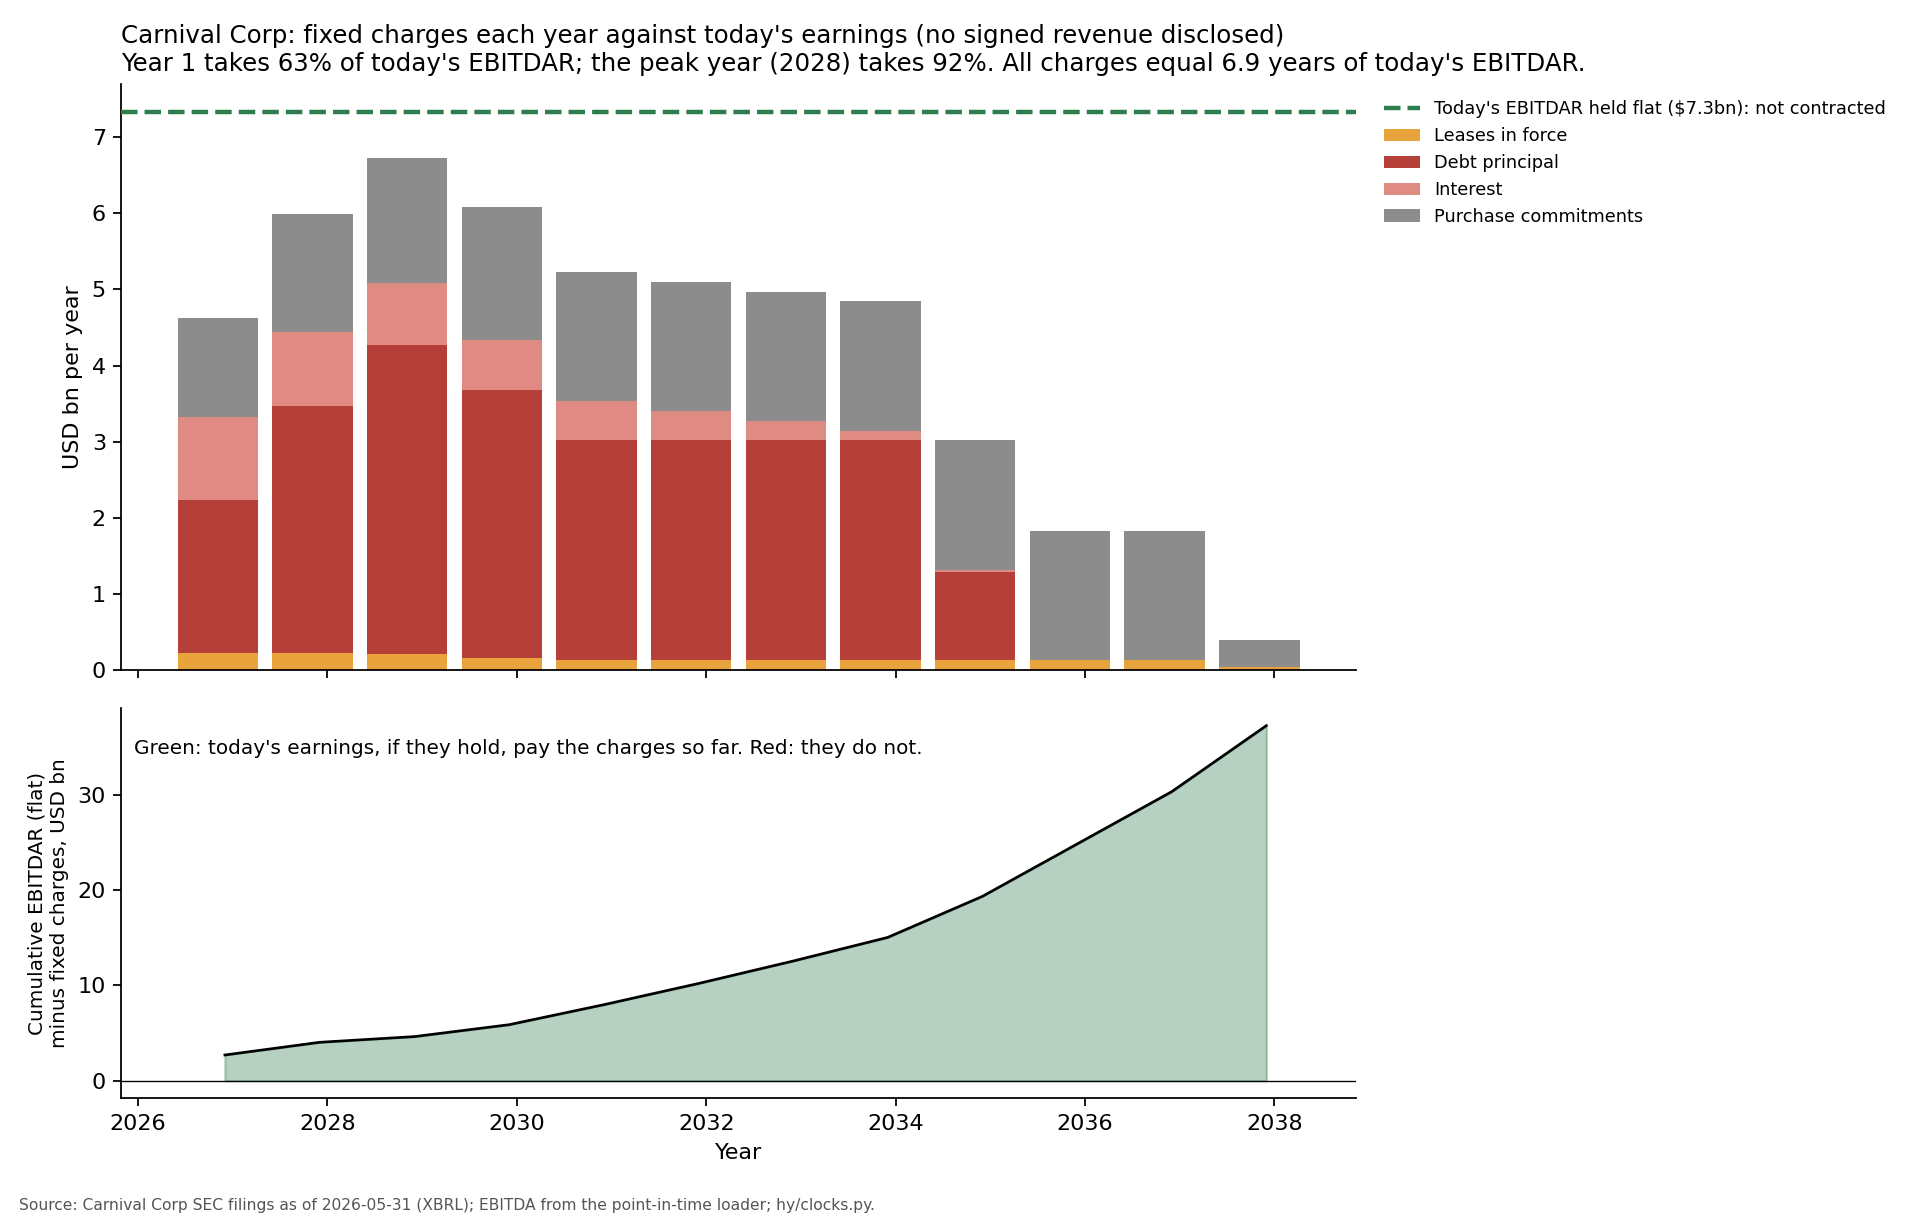
\includegraphics[width=0.95\linewidth]{figures/clocks_all_CCL.png}\caption*{The two clocks (section G2.1).}\end{figure}
\begin{figure}[H]\centering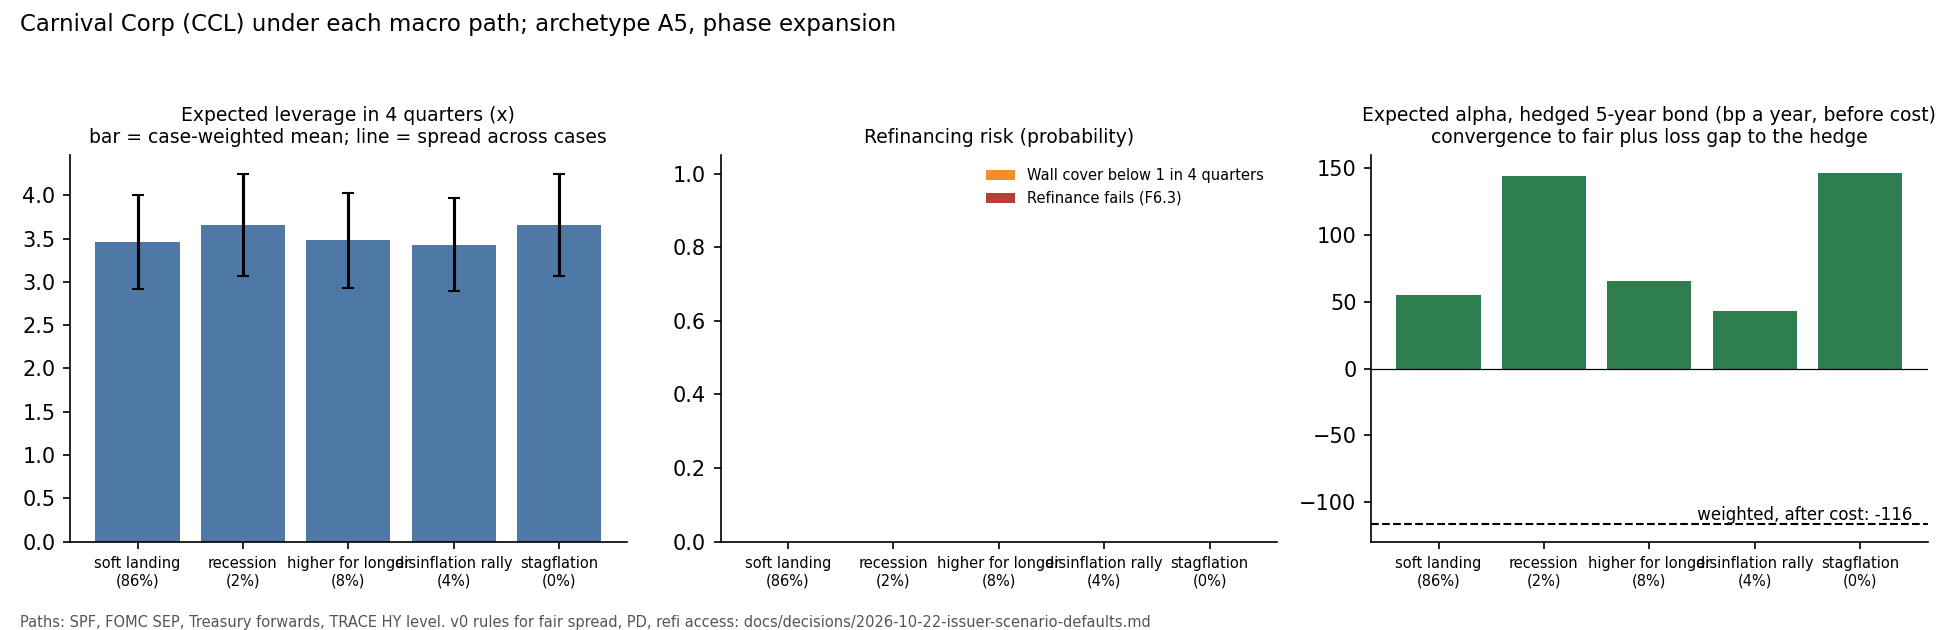
\includegraphics[width=0.95\linewidth]{figures/scenarios_CCL.png}\caption*{The company under each economic story (section G2.2).}\end{figure}
\begin{figure}[H]\centering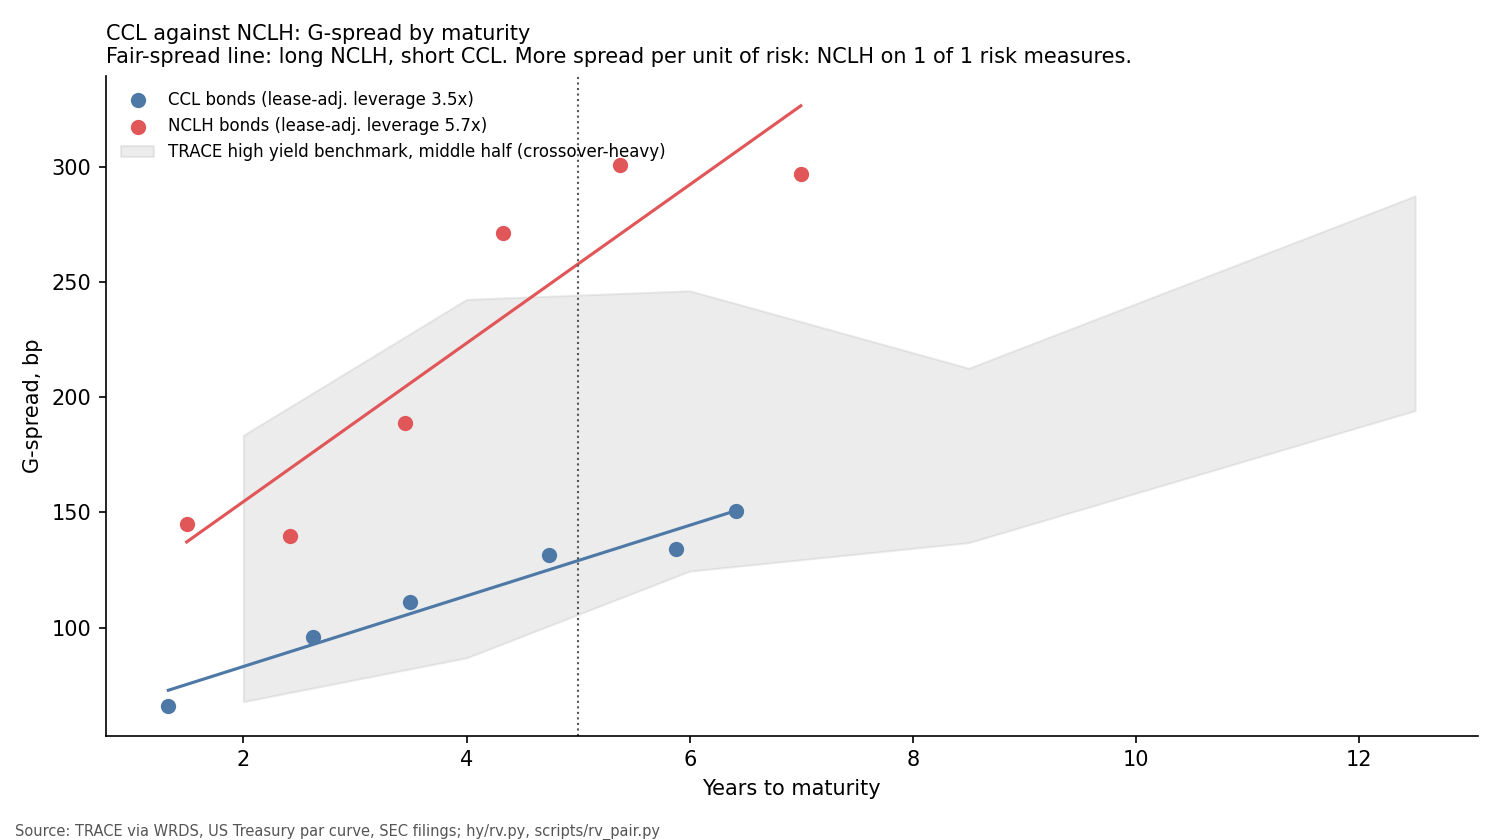
\includegraphics[width=0.85\linewidth]{figures/rv_CCL_NCLH.png}\caption*{The pair (section G2.3).}\end{figure}
\newpage
\section*{Norwegian Cruise Line Holdings (NCLH)}\pdfbookmark[1]{NCLH}{bm-NCLH}\label{memo-start-NCLH}
\par\noindent\fcolorbox{gray}{gray!6}{\parbox{\dimexpr\linewidth-2\fboxsep-2\fboxrule-1pt}{\sloppy \textbf{Recommendation.} Pass. This is a view of the company, not a trade: no gap between price and our view is bigger than the noise; the expected profit does not beat trading costs. If the money went elsewhere, the best alternative in this run is CCL. Position size and hedge: open until the call passes.}}

\subsection*{The combined view: four groups, one estimate}
Each group of methods estimates the same thing: what the bond should earn above a hedge, in bp a year. The combined estimate weighs the four groups. It ranks 5 of the issuers in this run. 2 of 5 groups point the same way as the combination.
\begin{center}\footnotesize\setlength{\tabcolsep}{3.5pt}\begin{tabular}{@{}lrrrl@{}}\toprule
Group & bp a year & Weight & Adds & Call \\\midrule
G1. Core process & -58 & 45\% & -26 & \textcolor{bad}{against owning} \\
G2 clocks. Two clocks & +102 & 20\% & +20 & \textcolor{amber}{leans to owning} \\
G2 rest. Built methods (rest) & +62 & 12\% & +7 & \textcolor{amber}{leans to owning} \\
G3. Credit skills & -215 & 12\% & -25 & \textcolor{bad}{against owning} \\
G4. Books & +11 & 12\% & +1 & \textcolor{amber}{leans to owning} \\
\textbf{Combined, before trading costs} &  &  & \textbf{-22} &  \\
Trading costs &  &  & -168 &  \\
\textbf{Combined, after trading costs} &  &  & \textbf{-190} &  \\
Weighted cases and stories alone, after costs &  &  & -100 &  \\
Calibrated: after-cost number x measured slope 0.079 &  &  & -15 &  \\
\bottomrule\end{tabular}\end{center}
Against the weighted cases and stories alone, the combination is 90 bp a year lower: the other methods take away from the case for owning the bond. A group that supports owning must beat the trading costs on its own. The weights are the user's choice: core process 45\%, two clocks 20\%, and 11.7\% each for the rest of the built methods, the credit skills and the books. The backtest alone would have put most weight on the built methods.
\par\noindent\fcolorbox{gray}{gray!6}{\parbox{\dimexpr\linewidth-2\fboxsep-2\fboxrule-1pt}{\sloppy \textbf{Alpha sizes are uncalibrated.} The backtest (2008 to 2026) shows that this kind of estimate ranks bonds well but overstates the size of the move. Realised alpha has been about 0.08 times the predicted alpha (standard error 0.05; 0.25 since 2019). The calibrated number multiplies by that slope: -15 bp a year after costs (-48 on the 2019 slope). The slope is not above zero by two standard errors, so the number ranks the bond but does not size it. Decision page: 2026-10-22-alpha-backtest-design. The backtest has no default-loss term yet.}}

\section*{G1. Core process: Gatto's steps, our method and rulebook, the relative value paper}
\par\noindent\fcolorbox{gray}{gray!6}{\parbox{\dimexpr\linewidth-2\fboxsep-2\fboxrule-1pt}{\sloppy \textbf{Verdict: \textcolor{bad}{against owning}.} This group reads Gatto's seven steps, our method and rulebook, and the relative value paper. Its estimate of expected profit is -58 bp a year before trading costs (costs are 168 bp a year); 3 of 4 of its weighted estimates point the same way. It carries 45\% of the combined view and ranks 8 of the issuers on this group alone. Best alternative for the same money: CCL.}}
\begin{center}\footnotesize\setlength{\tabcolsep}{3.5pt}\begin{tabular}{@{}p{6.2cm}rrrp{4.2cm}@{}}\toprule
Estimate & bp a year & Weight in group & Adds & Where it comes from \\\midrule
Default chance the price assumes (shown, weight 0) & -13 & 0\% & -0 & F9; mapping C2 \\
Earnings quality, add-backs, FCF check (can only lower) & -167 & 25\% & -42 & F3; ebitda-addback-treatment; hy-model-standards \\
Access to new money and the funding gap & -247 & 25\% & -62 & F4; RV PDF E75-E76 \\
Debt against market value & -264 & 25\% & -66 & F7.7 \\
Return above cash, repriced in every story & +445 & 25\% & +111 & RV PDF E50-E60; C1, C3 \\
\bottomrule\end{tabular}\end{center}
\subsection*{G1.1 Thesis}
The bond pays 258 bp over Treasuries at 5 years. A company with its leverage (5.7x with leases) pays 208 bp on the fair line, so the bond is cheap by 50 bp. What would reveal it, and when: open question.
\subsection*{G1.2 The business}
\begin{enumerate}
\item \textbf{What it sells:} History and Development of the Company Norwegian commenced operations from Miami, Florida in 1966, launching the modern cruise industry by offering weekly departures from Miami, Florida to destinations in the Caribbean. In February 2011, NCLH, a Bermuda limited company, was formed.
\item \textbf{How it earns:} revenue 10.2bn a year at a 27\% EBITDA margin.
\item \textbf{What it must spend to stand still:} rent of about \$0.0bn a year, plus maintenance capital spending.
\item \textbf{Competition:} open question.
\item \textbf{What breaks it:} contracts roll off or churn; the asset value cycle turns.
\end{enumerate}
Business type: A5.
\subsection*{G1.3 Earnings, normalised}
Last 12 months: EBITDA \$2.7bn at a 27\% margin; margin trend over 8 quarters -0.5 (t-statistic: above 1 rising, below $-1$ falling). One-off items \$-0.2bn. Free cash flow \$-1.2bn: -44\% of EBITDA. Earnings-quality flags raised: EQ7 conversion, EQ5 recurrence (of 4 tests the data supports). The add-back detail is in section G3.1.
\subsection*{G1.4 Cash, the funding gap, and the refinancing shock}
\begin{center}\footnotesize\setlength{\tabcolsep}{3.5pt}\begin{tabular}{@{}lr@{}}\toprule
Item & Value \\\midrule
Cash & \$0.2bn \\
Unused credit lines (tagged) & \$0.0bn \\
Less cash needed to run & \$0.1bn \\
Liquidity & \$0.2bn \\
Runway at today's cash burn, all capital spending (quarters) & 0.6 \\
First quarter cash runs out, severe case, maintenance spending only & 2 \\
First quarter cash runs out, severe case, all committed spending & 1 \\
\textbf{Runway we quote (the shortest)} & \textbf{0.6} (static) \\
Debt due in the next 18 months & \$1.6bn \\
Cash to meet debt due in a year, base case & 1.80x \\
Refinancing access score, likely story (0 to 6) & 3 \\
\bottomrule\end{tabular}\end{center}
\textbf{Funding gap if no lender refinances.} We add cash, the unused lines and the free cash flow of the cases, then take off the debt as it falls due, quarter by quarter. The minimum cash kept back is one month of cash operating costs (\$0.7bn).
\begin{center}\footnotesize\setlength{\tabcolsep}{3.5pt}\begin{tabular}{@{}lr@{}}\toprule
Measure & Value \\\midrule
Lowest point, likely story (maintenance spending only) & \$-1.0bn \\
First quarter below zero, likely story & quarter 1 \\
Lowest point with all capital spending & \$-2.0bn \\
First quarter below zero with all capital spending & quarter 1 \\
Lowest point, severe case & \$-2.5bn \\
Severe case with all capital spending: first quarter below zero & quarter 1 \\
Lowest point, weighted over the stories & \$-1.0bn \\
Debt due inside 8 quarters, share of all debt & 10\% \\
\bottomrule\end{tabular}\end{center}
\textbf{Refinancing shock.} \$1.6bn falls due in the next two years. It pays about 6.12\% today (TRACE coupons of bonds due inside 27 months). Refinanced at the forecast Treasury rate plus today's spread, yearly interest changes by \$0.0bn (0.9\% of EBITDA). Interest cover after refinancing: n/a; after capital spending n/a. Free cash flow after the shock: -7.8\% of debt.
\subsection*{G1.5 Debt: going-concern view}
\begin{center}\footnotesize\setlength{\tabcolsep}{3.5pt}\begin{tabular}{@{}lr@{}}\toprule
Measure & Value \\\midrule
Debt & \$15.5bn \\
Lease liabilities & \$0.0bn \\
EBITDA, last 12 months & \$2.7bn \\
Debt / EBITDA & 5.7x \\
(Debt + leases) / (EBITDA + rent) & 5.7x \\
Net debt / EBITDA & 5.6x \\
Coverage (after all capital spending) & n/a \\
Fixed-charge cover (after maintenance spending) & n/a \\
\bottomrule\end{tabular}\end{center}
\begin{center}\footnotesize\setlength{\tabcolsep}{3.5pt}\begin{tabular}{@{}lrrrrr@{}}\toprule
Bond & Coupon & Matures & Price & Yield & Spread (bp) \\\midrule
62888HAA7 & 6.12\% & 2028-03-15 & 100.2 & 5.98\% & 145 \\
62886HBG5 & 7.75\% & 2029-02-15 & 103.3 & 6.10\% & 140 \\
62886HBP5 & 6.25\% & 2030-03-01 & 98.8 & 6.64\% & 189 \\
62886HBY6 & 5.87\% & 2031-01-15 & 94.1 & 7.48\% & 271 \\
62886HBR1 & 6.75\% & 2032-02-01 & 95.4 & 7.80\% & 301 \\
62886HBZ3 & 6.25\% & 2033-09-15 & 91.6 & 7.83\% & 297 \\
\bottomrule\end{tabular}\end{center}
Claims view (who is paid what in a default): open question until the debt documents are read.
\subsection*{G1.6 Company value}
Market value of the whole company \$25bn (shares \$10bn plus net debt): 9.2x EBITDA; debt is 62\% of it. Our own valuation range and the bonds' recovery if the company defaults: open questions (they need a peer set and a distressed multiple).
\subsection*{G1.7 The decision against cash}
We put the same money in the bond nearest five years (62886HBR1, 6.75\% due 2032-02-01, price 95.44 plus 0.85 accrued) or in six-month Treasury bills at 4.20\%. In each story the bond either survives and is repriced, or defaults and returns 35 per 100 (a 40\% recovery paid a year later, valued at 15\% a year). In default the holder loses 64\% of the price paid.
\begin{center}\footnotesize\setlength{\tabcolsep}{3.5pt}\begin{tabular}{@{}lr@{}}\toprule
Measure & Value \\\midrule
Expected return above cash, bp a year & +445 \\
Chance of a loss over six months & 11.5\% \\
Chance of doing worse than cash & 11.5\% \\
Average loss in the worst 5\% of outcomes & 15.8\% \\
Same, with rates and the market hedged out, bp a year & +143 \\
Best alternative in this run (worst 5\% loss within the 25\% budget) & CCL \\
Return given up against that alternative, bp a year & -292 \\
\bottomrule\end{tabular}\end{center}
\section*{G2. Built methods: two clocks, stories and cases, relative value, the gate}
\par\noindent\fcolorbox{gray}{gray!6}{\parbox{\dimexpr\linewidth-2\fboxsep-2\fboxrule-1pt}{\sloppy \textbf{Verdict: \textcolor{amber}{leans to owning}.} This group reads the spread level, the fair line and the pair, the economic stories, the health panel. Its estimate of expected profit is +62 bp a year before trading costs (costs are 168 bp a year); 4 of 5 of its weighted estimates point the same way. It carries 12\% of the combined view and ranks 2 of the issuers on this group alone. Gate: pass.}}
\begin{center}\footnotesize\setlength{\tabcolsep}{3.5pt}\begin{tabular}{@{}p{6.2cm}rrrp{4.2cm}@{}}\toprule
Estimate & bp a year & Weight in group & Adds & Where it comes from \\\midrule
Spread level: the extra pay over the market (carry) & +90 & 42\% & +38 & Spec S14 E0; K15 \\
Weighted cases and stories & +68 & 25\% & +17 & M5.4, M7.5 \\
Spread against the fair line & +117 & 17\% & +19 & M7.4, M7.5 \\
The pair & +22 & 8\% & +2 & M7.4; F10 S4 \\
Health panel & -162 & 8\% & -13 & F8 \\
\bottomrule\end{tabular}\end{center}
\subsection*{G2.1 The two clocks: bills against what pays for them}
\par\noindent\fcolorbox{gray}{gray!6}{\parbox{\dimexpr\linewidth-2\fboxsep-2\fboxrule-1pt}{\sloppy \textbf{Verdict: \textcolor{amber}{leans to owning}.} This group reads the bills the company owes against the revenue customers have signed for. Its estimate of expected profit is +102 bp a year before trading costs (costs are 168 bp a year); 1 of 1 of its weighted estimates point the same way. It carries 20\% of the combined view and ranks 3 of the issuers on this group alone. The clocks count as their own bucket in the combined view.}}
\begin{center}\footnotesize\setlength{\tabcolsep}{3.5pt}\begin{tabular}{@{}p{6.2cm}rrrp{4.2cm}@{}}\toprule
Estimate & bp a year & Weight in group & Adds & Where it comes from \\\midrule
The two clocks & +102 & 100\% & +102 & M4.7 \\
\bottomrule\end{tabular}\end{center}
Fixed bills total \$17.6bn, centred 5.6 years out: leases in force \$2.2bn, debt principal \$15.5bn. That is 6.5 years of today's EBITDAR; next year's bills take 41\% of it.
The company discloses no material signed revenue, so the second clock is today's earnings held flat (chart at the end).
\subsection*{G2.2 Economic stories and cases}
Cases on the most likely story (soft landing), stage of the cycle: expansion.
\begin{center}\scriptsize\setlength{\tabcolsep}{3.5pt}\begin{tabular}{@{}lrrrrrrr@{}}\toprule
Case & Weight & Growth / qtr & Leverage in 1 yr & Peak leverage & Lowest liquidity & Cash runs out & Refi fails \\\midrule
base & 64\% & 1.5\% & 5.2x & 6.3x & \$0.4bn & no & no \\
down moderate & 11\% & 1.9\% & 6.1x & 6.8x & \$0.3bn & no & no \\
down severe & 4\% & 1.8\% & 8.6x & 8.6x & \$-0.2bn & 2 & no \\
upside & 21\% & 1.8\% & 4.4x & 5.8x & \$0.5bn & no & no \\
\bottomrule\end{tabular}\end{center}
\begin{center}\scriptsize\setlength{\tabcolsep}{3.5pt}\begin{tabular}{@{}lrrrrrr@{}}\toprule
Story & Chance & Leverage in 1 yr & Peak leverage (down) & Refi fails & Default chance & Expected profit (bp/yr) \\\midrule
soft landing & 86\% & 5.3x & 8.6x & 0\% & 2.3\% & 61 \\
recession & 2\% & 5.6x & 9.2x & 100\% & 3.7\% & 300 \\
higher for longer & 8\% & 5.3x & 8.7x & 0\% & 2.3\% & 100 \\
disinflation rally & 4\% & 5.2x & 8.6x & 0\% & 2.3\% & 15 \\
stagflation & 0\% & 5.6x & 9.2x & 100\% & 4.4\% & 265 \\
\bottomrule\end{tabular}\end{center}
\subsection*{G2.3 Relative value and the pair}
Fair line: log spread = -5.64 + 0.312 x leverage, fitted on 8 issuers in this run. 5-year spread 258 bp against a fair 208 bp.
\textbf{Against peers.} Peers are the high yield bonds that traded in 2026-08-31 (733 bonds with leverage on file), in the same 3 to 7 year maturity bucket. Sector: Consumer Discretionary. Rating class: B (implied by leverage). A positive value means the issuer pays more than the median peer.
\begin{center}\footnotesize\setlength{\tabcolsep}{3.5pt}\begin{tabular}{@{}lrr@{}}\toprule
Peer group & Excess spread to peers (ESP) & Spread per turn against peers (E13) \\\midrule
Sector and rating & +28\% & +33\% \\
Sector only & +56\% & +56\% \\
Rating only & +55\% & +42\% \\
\bottomrule\end{tabular}\end{center}
\textbf{SPiDER} (spread per unit of debt to 10-year average EBITDA; Dynkin et al. 2021, ch. 14): cheaper than 20\% of the peer bonds across all sectors, and -69\% against sector and rating peers. It has no weight in the score: its edge beyond spread level is small (t 1.3 at 12 months).
\textbf{Against CCL.} Spreads at 5 years: CCL 129 bp, NCLH 258 bp.
\begin{center}\footnotesize\setlength{\tabcolsep}{3.5pt}\begin{tabular}{@{}lrrr@{}}\toprule
Spread per & CCL & NCLH & Cheaper \\\midrule
turn of leverage & 37 & 45 & NCLH \\
\bottomrule\end{tabular}\end{center}
The fair line favours long NCLH, short CCL: a gap of 3 bp, which halves in about 3 weeks on six months of trades. Under the stories the pair earns soft landing +6, recession +156, higher for longer +35, disinflation rally -28, stagflation +118 bp a year; weighted +11 bp before costs.
\subsection*{G2.4 Expected profit and price against our view}
Hedged 5-year bond over six months: 68 bp a year before trading costs, -100 bp after. It does not beat costs. The expected default loss is charged on the price paid: 64\% of it in default, not 60\% of face.
\begin{center}\footnotesize\setlength{\tabcolsep}{3.5pt}\begin{tabular}{@{}p{5.2cm}rrrrl@{}}\toprule
Question & Price assumes & Our view & Gap & Noise & Gap bigger than noise? \\\midrule
Default chance at the v0 price of risk (shown, not tested) & 2.1\% & 2.3\% & 0.2\% & open & not tested \\
Breakeven default probability, 12 months (loss on price) & 4.0\% & 2.3\% & -1.7\% & 2.0\% & no \\
Leverage the spread is pricing & 6.37 & 5.68 & -0.69 & 0.90 & no \\
Spread against fair (bp) & 258 & 208 & -50 & 58 & no \\
Rating class & open & BB & open & open & not tested \\
Recovery if default (per 1 of face, discounted for delay) & open & 0.35 & open & open & not tested \\
\bottomrule\end{tabular}\end{center}
The first row turns the spread into a default chance with a fixed price of risk. That is not a real default chance, so it is shown but not tested. The breakeven row asks a cleaner question: is our default chance below the rate at which the spread only just pays for default losses?
\subsection*{G2.5 Risks and the health panel}
\begin{itemize}\item Little of the earnings turns into free cash. Tracked by: cash conversion (fcf / ebitda) (-0.44). Resolves when: growth spending ends.\item Free cash flow repays little debt. Tracked by: free cash flow / debt (-0.08). Resolves when: free cash flow turns positive.\end{itemize}
\begin{center}\footnotesize\setlength{\tabcolsep}{3.5pt}\begin{tabular}{@{}lrl@{}}\toprule
Measure & Value & Band \\\midrule
Cash conversion (FCF / EBITDA) & -0.44 & \textcolor{bad}{red} \\
Free cash flow / debt & -0.08 & \textcolor{bad}{red} \\
Refinancing access score (0 to 6) & 3.00 & \textcolor{amber}{amber} \\
Earnings-quality flags & 2.00 & \textcolor{amber}{amber} \\
Margin trend (t-statistic) & -0.46 & \textcolor{amber}{amber} \\
Chance debt due in 1 year is not covered & 0.15 & \textcolor{amber}{amber} \\
Cash to meet debt due in 1 year (base case) & 1.80 & \textcolor{good}{green} \\
Weight on the downside cases & 0.15 & \textcolor{good}{green} \\
Chance cash runs out within 2 years & 0.04 & \textcolor{good}{green} \\
Coverage & n/a & n/a \\
Fixed-charge cover & n/a & n/a \\
\bottomrule\end{tabular}\end{center}
\section*{G3. Credit skills: the lender's checklists applied to a public bond}
\par\noindent\fcolorbox{gray}{gray!6}{\parbox{\dimexpr\linewidth-2\fboxsep-2\fboxrule-1pt}{\sloppy \textbf{Verdict: \textcolor{bad}{against owning}.} This group reads the lender's checklists: add-backs, covenants, watchlist, trend, memo structure. Its estimate of expected profit is -215 bp a year before trading costs (costs are 168 bp a year); 1 of 1 of its weighted estimates point the same way. It carries 12\% of the combined view and ranks 6 of the issuers on this group alone. Its estimates can only lower the combined number: a clean checklist earns no credit. Watchlist: watchlist.}}
\begin{center}\footnotesize\setlength{\tabcolsep}{3.5pt}\begin{tabular}{@{}p{6.2cm}rrrp{4.2cm}@{}}\toprule
Estimate & bp a year & Weight in group & Adds & Where it comes from \\\midrule
Watchlist tier (can only lower) & -215 & 100\% & -215 & borrower-monitoring; covenant-compliance \\
\bottomrule\end{tabular}\end{center}
\subsection*{G3.1 Add-backs and their cash effect}
Reported EBITDA over the last 12 months is \$2.6bn. The company's own measure adds back \$0.2bn of one-off items to reach \$2.7bn: 6.5\% of reported EBITDA (a negative figure is a one-off gain taken out). This is above the 5\% line the lender's checklist sets for one item. They do not recur in three quarters running. If every add-back were paid in cash, free cash flow would be \$-1.4bn. The two roads to free cash flow (the EBITDA bridge, n/a; operating cash flow less capital spending, \$-1.2bn) differ by n/a of EBITDA: within the 10\% tolerance. The add-back table by category is an open question: the data has one total line.
\subsection*{G3.2 Covenant headroom}
The filing states these maintenance tests. We test them on our own ratio, which uses our EBITDA, not the covenant's, and the whole group.
\begin{center}\footnotesize\setlength{\tabcolsep}{3.5pt}\begin{tabular}{@{}p{3.8cm}rrrp{1.9cm}p{4.4cm}@{}}\toprule
Test & Level & Our ratio & Headroom & Band & Notes \\\midrule
an EBITDA to consolidated debt service ratio & 1.25 & n/a & n/a & open & only tested below a trigger; EBITDA / (cash interest + debt due in 12 months) \\
free liquidity & 250.00 & 218.10 & -15\% & proxy only (open) & our ratio is only a bound for this test; cash only (unused lines not tagged) \\
\bottomrule\end{tabular}\end{center}
No test can be read on our own ratio: each one binds a narrower group of debt or needs the credit lines. Headroom stays an open question; it does not move the watchlist.
\subsection*{G3.3 Watchlist and trajectory}
Watchlist tier: \textbf{watchlist} because free cash flow is negative. EBITDA against the same months a year earlier: 10.3\% (no plan is public, so last year stands in for it). Open: liquidity against debt due cannot be read: revolver capacity not tagged.
\begin{center}\footnotesize\setlength{\tabcolsep}{3.5pt}\begin{tabular}{@{}llll@{}}\toprule
Measure & Direction & How much weight & Change on a year earlier, last quarter \\\midrule
revenue & improving & trend & 4.9\% \\
EBITDA & deteriorating & observation & -1.5\% \\
EBITDA margin & deteriorating & observation & -6.1\% \\
cash conversion & deteriorating & observation & -61.4\% \\
\bottomrule\end{tabular}\end{center}
One quarter is an observation, two a data point, three or four a trend. The measures point different ways; the memo must explain why.
\subsection*{G3.4 Memo structure check}
\begin{center}\footnotesize\setlength{\tabcolsep}{3.5pt}\begin{tabular}{@{}lp{9cm}l@{}}\toprule
Section & Requires & Status \\\midrule
Executive summary & the business in one sentence, the opportunity, 2 to 3 reasons, 2 to 3 risks & \textcolor{good}{pass} \\
Capital structure & each tranche with face, coupon, maturity; senior, total and net leverage; LTV & \textcolor{amber}{open} \\
Terms & maintenance covenant levels and test dates; incurrence baskets; call terms & \textcolor{amber}{open} \\
Investment merits & free cash flow generation and the base-case deleveraging path & \textcolor{good}{pass} \\
Key risks & 3 to 5 issuer-specific risks, each with a mitigant & \textcolor{good}{pass} \\
Historical financials & at least 3 years, quarterly where available & \textcolor{good}{pass} \\
EBITDA adjustments & reported-to-adjusted bridge with the load as a share of EBITDA and the 5\% flag & \textcolor{amber}{open} \\
Model output & base and downside: EBITDA, FCF, leverage path, covenant headroom, liquidity runway & \textcolor{amber}{open} \\
\bottomrule\end{tabular}\end{center}
\textbf{Rules that do not transfer to a public bond:}\begin{itemize}\item The compliance certificate is the source of truth; public bonds have none. Headroom here uses our own ratio against a level parsed from the filing text. (covenant-compliance)\item Equity cures, step-down schedules and window-dressing checks need the credit agreement and monthly revolver balances. (covenant-compliance)\item Performance against the sponsor plan: no plan is public. The proxy is the same quarters a year earlier. (borrower-monitoring)\item Add-back caps and the certificate reconciliation live in the credit agreement. Compustat gives one special-items line, not the category table. (ebitda-addback-treatment)\item Sources and uses at entry, the sponsor case and the management call apply to new loans, not to bonds bought in the secondary market. (credit-memo-standards)\item Monthly lender packages do not exist for public issuers; XBRL quarters replace them. (quarterly-package-extraction)\end{itemize}
\section*{G4. Books: Kricheff, and Ganguin and Bilardello (S\&P)}
\par\noindent\fcolorbox{gray}{gray!6}{\parbox{\dimexpr\linewidth-2\fboxsep-2\fboxrule-1pt}{\sloppy \textbf{Verdict: \textcolor{amber}{leans to owning}.} This group reads Kricheff's cash bridge and ratios; the S\&P risk profiles and rating anchor. Its estimate of expected profit is +11 bp a year before trading costs (costs are 168 bp a year); 1 of 2 of its weighted estimates point the same way. It carries 12\% of the combined view and ranks 4 of the issuers on this group alone. S\&P anchor class: BB.}}
\begin{center}\footnotesize\setlength{\tabcolsep}{3.5pt}\begin{tabular}{@{}p{6.2cm}rrrp{4.2cm}@{}}\toprule
Estimate & bp a year & Weight in group & Adds & Where it comes from \\\midrule
Spread against the S\&P risk score & +23 & 50\% & +11 & Ganguin and Bilardello ch. 10 \\
Spread per turn of leverage (with the trap guard) & +0 & 50\% & +0 & Kricheff ch. 21 \\
\bottomrule\end{tabular}\end{center}
\subsection*{G4.1 Kricheff's cash-flow bridge and ratio set}
\begin{center}\footnotesize\setlength{\tabcolsep}{3.5pt}\begin{tabular}{@{}lr@{}}\toprule
Line (last 12 months) & Value \\\midrule
Adjusted EBITDA & \$2.7bn \\
less capital spending & \$3.3bn \\
less cash interest & n/a \\
less cash taxes & \$0.0bn \\
less increase in working capital & \$-0.1bn \\
\textbf{Free cash flow} & \textbf{n/a} \\
Check: free cash flow before capital spending less operating cash flow & n/a \\
Free cash flow after dividends & open (dividends not loaded) \\
\bottomrule\end{tabular}\end{center}
\begin{center}\footnotesize\setlength{\tabcolsep}{3.5pt}\begin{tabular}{@{}lrlr@{}}\toprule
Ratio & Value & Ratio & Value \\\midrule
EBITDA / cash interest & n/a & Debt / EBITDA & 5.7x \\
(EBITDA $-$ capex) / interest & n/a & Net debt / EBITDA & 5.6x \\
(EBITDA $-$ maintenance capex) / interest & n/a & Free cash flow / debt & -8.0\% \\
EBITDA / debt (highest rate at 1x cover) & 18.0\% & Market value / EBITDA & 9.2x \\
Equity cushion (1 $-$ debt / market value) & 38\% & Spread per turn of leverage & 45 bp \\
\bottomrule\end{tabular}\end{center}
Kricheff's snapshot rule: operating cash flow does not cover capital spending, so the issuer lives on the capital markets and needs the detailed liquidity work of section G1.4. Spread per turn compares the bond with the run's median of 38 bp a turn. Kricheff warns that a high spread per turn can mean weak cash flow, not value; read it with free cash flow / debt. The book measures leverage through each bond's rank; with no face by rank, total leverage stands in.
\subsection*{G4.2 The S\&P risk profiles and the rating anchor}
S\&P adds leases to debt and scores each ratio against the median of each rating class (CreditStats 2002, from the book). Scores run from 1 (safest) to 10 (default).
\begin{center}\footnotesize\setlength{\tabcolsep}{3.5pt}\begin{tabular}{@{}lrrrr@{}}\toprule
Ratio & Value & Score & BB median & B median \\\midrule
Debt / (debt + market value of equity) & 61\% & 7.9 & 57.5\% & 78.5\% \\
Funds from operations / debt & 13\% & 8.9 & 19.5\% & 10.8\% \\
Free operating cash flow / debt & -8\% & 9.9 & 8.5\% & 2.5\% \\
EBITDA / interest (with lease interest) & n/a & n/a & 3.2x & 1.8x \\
EBITDA margin & 27\% & 3.0 &  &  \\
\bottomrule\end{tabular}\end{center}
Financial risk score 7.7. Business risk score 4.5: industry 5, steadiness of sales 3 (year-on-year growth varies by 4.1\%), customer spread 5. The book puts 45\% of the weight on business risk for this class, so the default risk score is 6.3: the \textbf{BB} class. The line from score to spread across the run did not slope upward, so it gives no estimate. The 2005 edition has no modern anchor table; its own weighting table stands in for it.
\section*{Coming events, open questions, and the record}
\begin{itemize}\item Next quarterly results (estimated from filing cadence): 2026-11-02 (estimate).\item Debt due by 0.5 years out:  - \$0.5bn.\end{itemize}
\textbf{Open questions, most important first:}\begin{enumerate}\item A dated catalyst that would close the gap (G2).\item The observable and level that would prove the call wrong (G8).\item Face amount of each tranche and the secured debt ahead of the bonds (debt note table).\item Claims view: allowed claims by class and the entity map (framework F5).\item Covenant 'free liquidity': our ratio is only a bound for this test (subsidiary group, narrower debt, or untagged credit lines); read the credit agreement definition.\item The funding gap opens only because no revolver capacity is tagged: read the credit facility note before using the gap.\item Revolver commitment, draw, and borrowing base: not tagged; read the credit agreement note.\item F4 points 3 (unencumbered assets) and 6 (sponsor support) are scored 0 until read.\item Recovery, delay and the required return on a defaulted claim are v0 (R = 0.4, tau = 1 year, k = 15\%); the claims view and documents replace them.\item Peer set of at least four issuers of the same archetype (F3.3) for the valuation range (F7.1).\end{enumerate}
\textbf{Record (filled at exit):} exit date; return against the rating-matched index; worst point against the index; reason; the rule that would have helped.
\newpage
\begin{figure}[H]\centering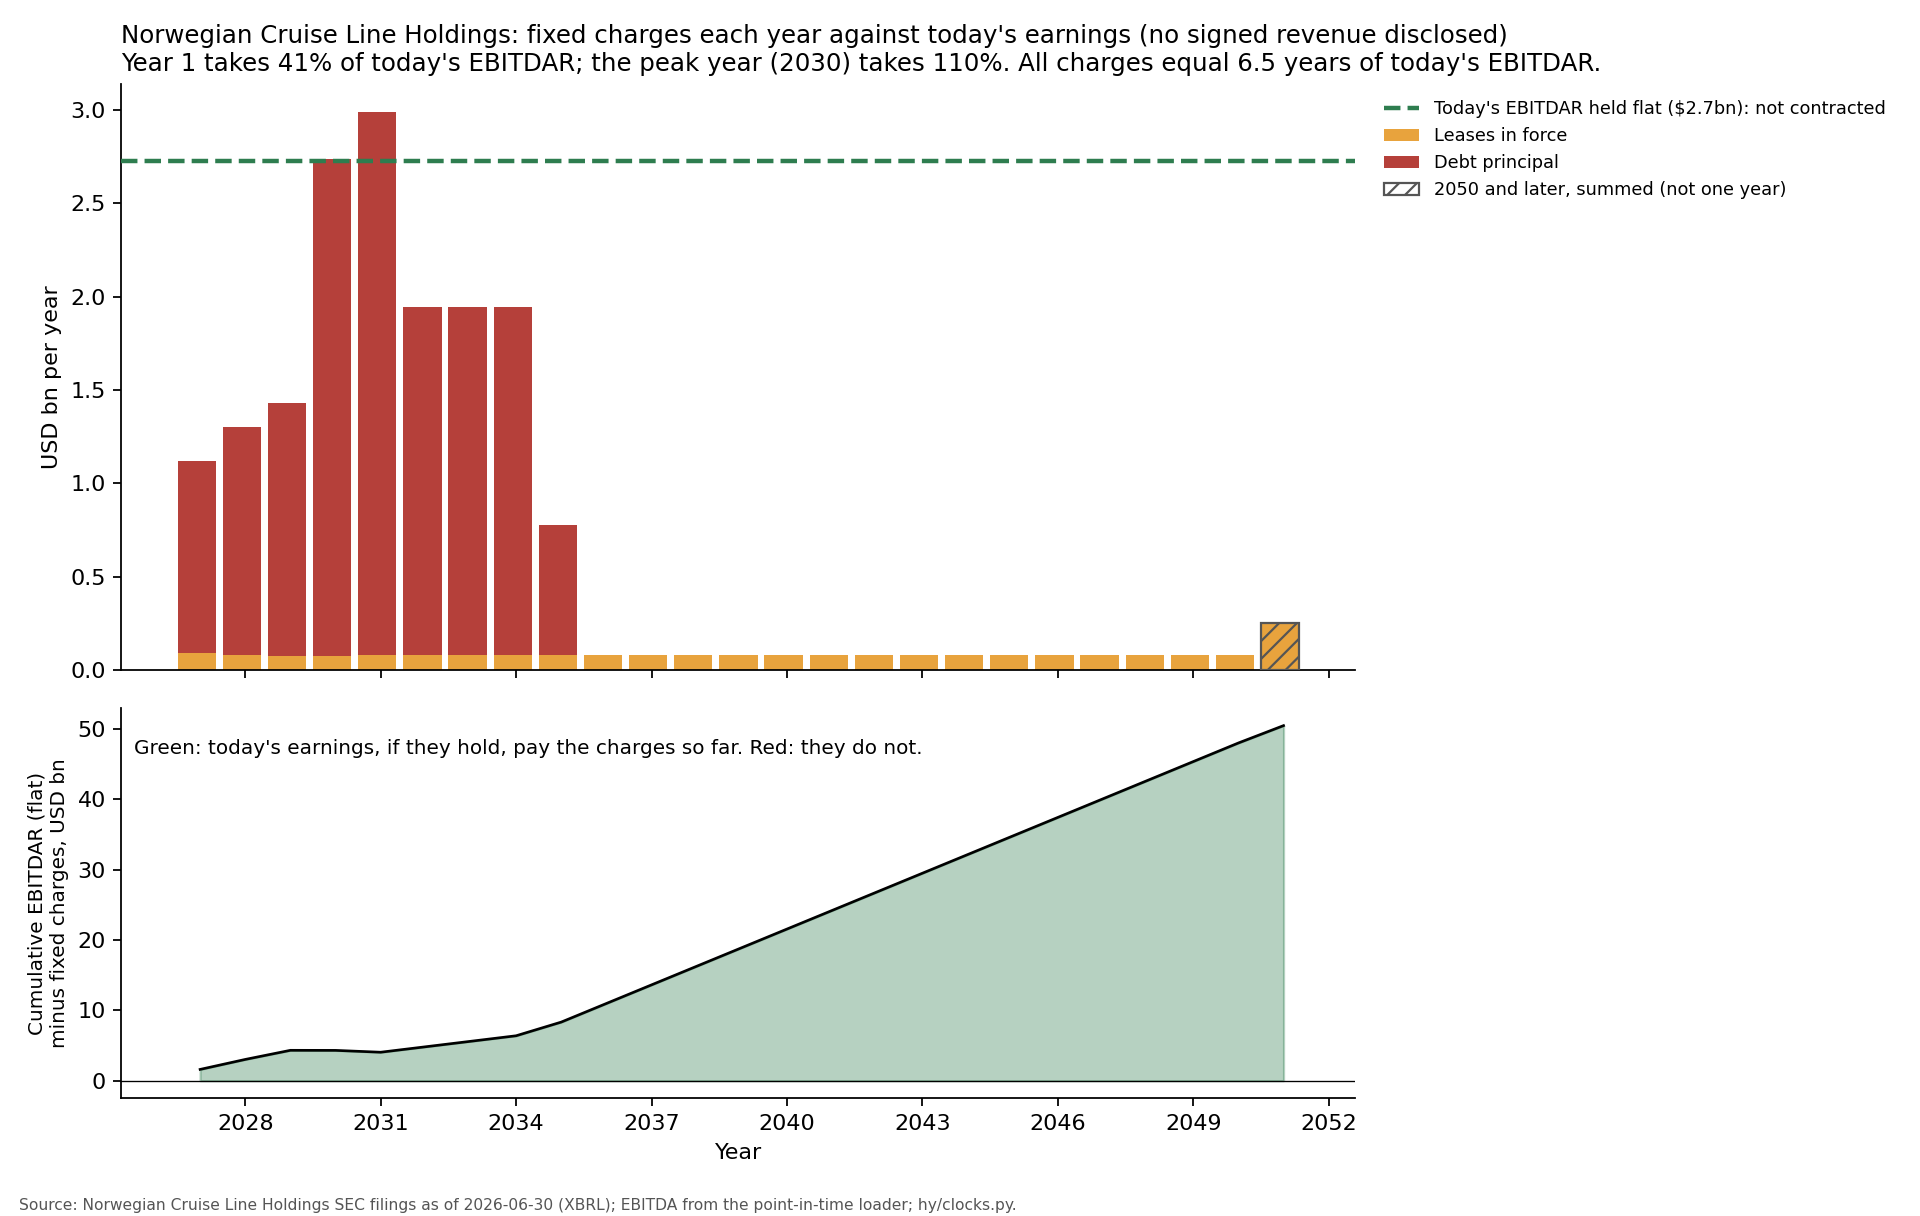
\includegraphics[width=0.95\linewidth]{figures/clocks_all_NCLH.png}\caption*{The two clocks (section G2.1).}\end{figure}
\begin{figure}[H]\centering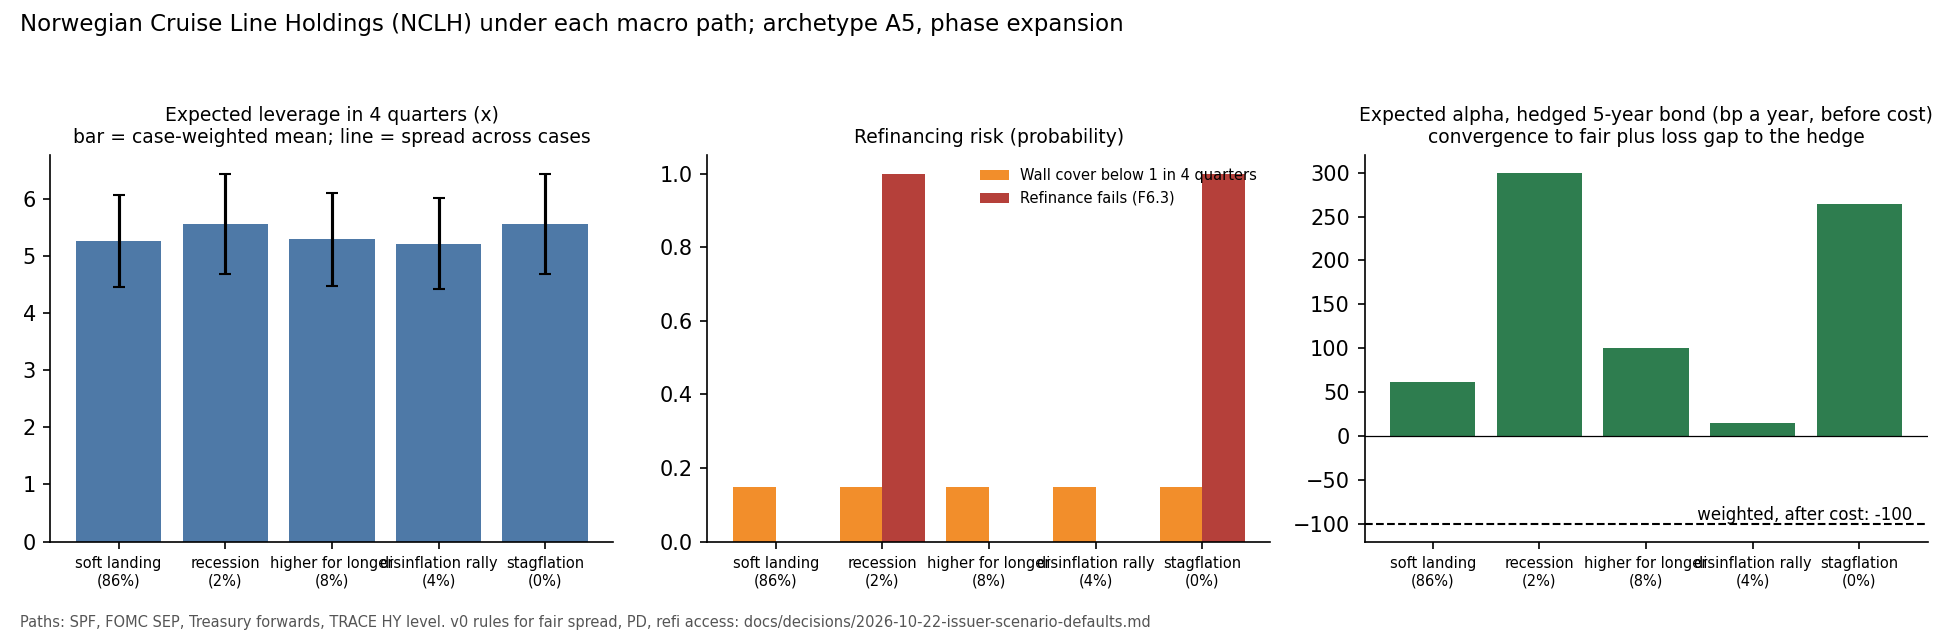
\includegraphics[width=0.95\linewidth]{figures/scenarios_NCLH.png}\caption*{The company under each economic story (section G2.2).}\end{figure}
\begin{figure}[H]\centering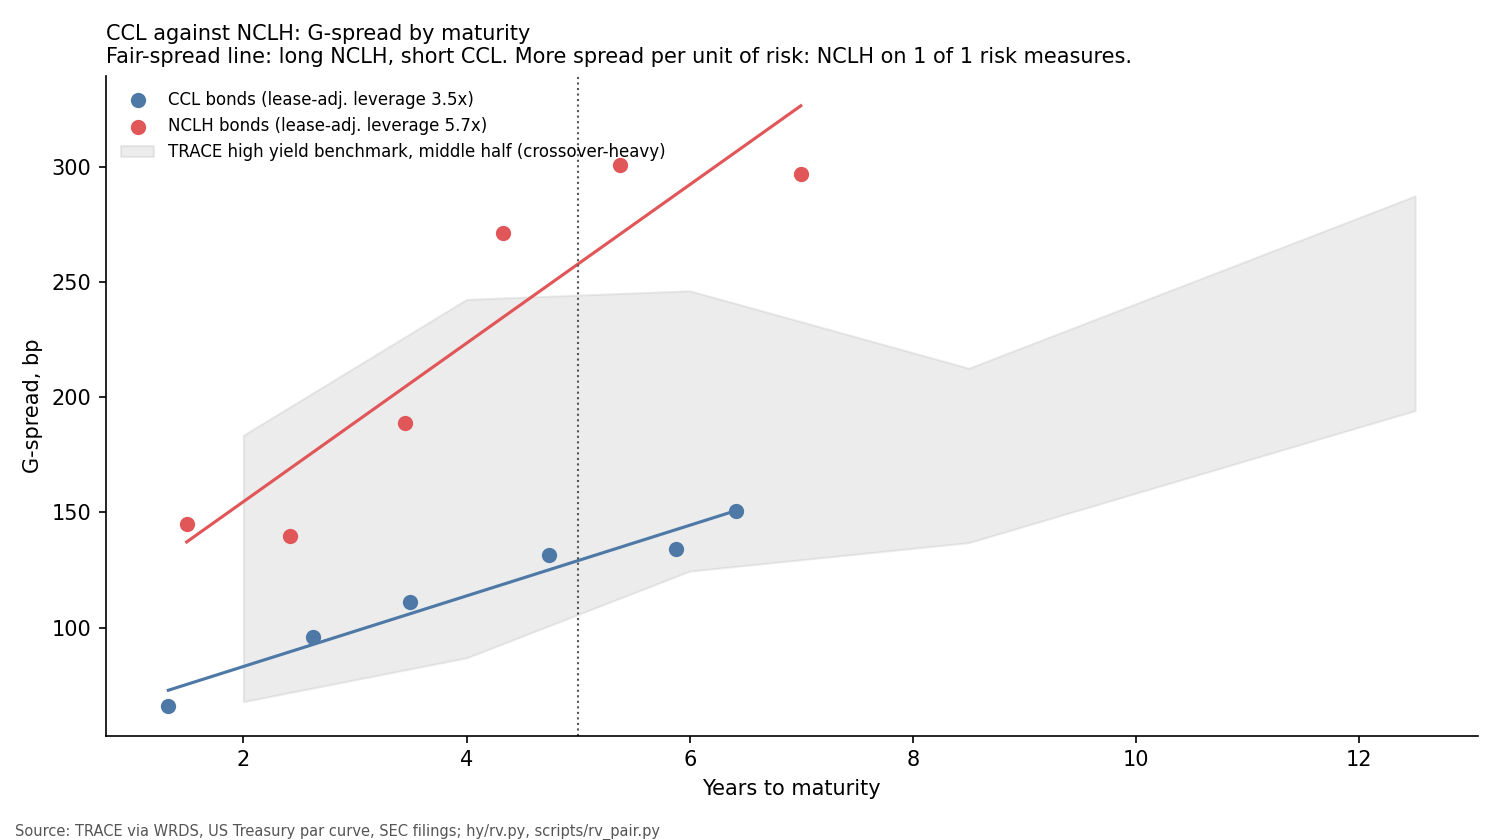
\includegraphics[width=0.85\linewidth]{figures/rv_CCL_NCLH.png}\caption*{The pair (section G2.3).}\end{figure}
\newpage
\section*{MGM Resorts International (MGM)}\pdfbookmark[1]{MGM}{bm-MGM}\label{memo-start-MGM}
\par\noindent\fcolorbox{gray}{gray!6}{\parbox{\dimexpr\linewidth-2\fboxsep-2\fboxrule-1pt}{\sloppy \textbf{Recommendation.} Pass. This is a view of the company, not a trade: the expected profit does not beat trading costs; the checks point in different directions. If the money went elsewhere, the best alternative in this run is NCLH. Position size and hedge: open until the call passes.}}

\subsection*{The combined view: four groups, one estimate}
Each group of methods estimates the same thing: what the bond should earn above a hedge, in bp a year. The combined estimate weighs the four groups. It ranks 8 of the issuers in this run. 4 of 5 groups point the same way as the combination.
\begin{center}\footnotesize\setlength{\tabcolsep}{3.5pt}\begin{tabular}{@{}lrrrl@{}}\toprule
Group & bp a year & Weight & Adds & Call \\\midrule
G1. Core process & -4 & 45\% & -2 & \textcolor{bad}{against owning} \\
G2 clocks. Two clocks & -108 & 20\% & -22 & \textcolor{bad}{against owning} \\
G2 rest. Built methods (rest) & -86 & 12\% & -10 & \textcolor{bad}{against owning} \\
G3. Credit skills & +0 & 12\% & +0 & \textcolor{good}{no objection} \\
G4. Books & -126 & 12\% & -15 & \textcolor{bad}{against owning} \\
\textbf{Combined, before trading costs} &  &  & \textbf{-48} &  \\
Trading costs &  &  & -172 &  \\
\textbf{Combined, after trading costs} &  &  & \textbf{-220} &  \\
Weighted cases and stories alone, after costs &  &  & -395 &  \\
Calibrated: after-cost number x measured slope 0.079 &  &  & -17 &  \\
\bottomrule\end{tabular}\end{center}
Against the weighted cases and stories alone, the combination is 175 bp a year higher: the other methods add to the case for owning the bond. A group that supports owning must beat the trading costs on its own. The weights are the user's choice: core process 45\%, two clocks 20\%, and 11.7\% each for the rest of the built methods, the credit skills and the books. The backtest alone would have put most weight on the built methods.
\par\noindent\fcolorbox{gray}{gray!6}{\parbox{\dimexpr\linewidth-2\fboxsep-2\fboxrule-1pt}{\sloppy \textbf{Alpha sizes are uncalibrated.} The backtest (2008 to 2026) shows that this kind of estimate ranks bonds well but overstates the size of the move. Realised alpha has been about 0.08 times the predicted alpha (standard error 0.05; 0.25 since 2019). The calibrated number multiplies by that slope: -17 bp a year after costs (-56 on the 2019 slope). The slope is not above zero by two standard errors, so the number ranks the bond but does not size it. Decision page: 2026-10-22-alpha-backtest-design. The backtest has no default-loss term yet.}}

\section*{G1. Core process: Gatto's steps, our method and rulebook, the relative value paper}
\par\noindent\fcolorbox{gray}{gray!6}{\parbox{\dimexpr\linewidth-2\fboxsep-2\fboxrule-1pt}{\sloppy \textbf{Verdict: \textcolor{bad}{against owning}.} This group reads Gatto's seven steps, our method and rulebook, and the relative value paper. Its estimate of expected profit is -4 bp a year before trading costs (costs are 172 bp a year); 2 of 4 of its weighted estimates point the same way. It carries 45\% of the combined view and ranks 6 of the issuers on this group alone. Best alternative for the same money: NCLH.}}
\begin{center}\footnotesize\setlength{\tabcolsep}{3.5pt}\begin{tabular}{@{}p{6.2cm}rrrp{4.2cm}@{}}\toprule
Estimate & bp a year & Weight in group & Adds & Where it comes from \\\midrule
Default chance the price assumes (shown, weight 0) & -26 & 0\% & -0 & F9; mapping C2 \\
Earnings quality, add-backs, FCF check (can only lower) & -167 & 25\% & -42 & F3; ebitda-addback-treatment; hy-model-standards \\
Access to new money and the funding gap & +96 & 25\% & +24 & F4; RV PDF E75-E76 \\
Debt against market value & +66 & 25\% & +17 & F7.7 \\
Return above cash, repriced in every story & -13 & 25\% & -3 & RV PDF E50-E60; C1, C3 \\
\bottomrule\end{tabular}\end{center}
\subsection*{G1.1 Thesis}
The bond pays 175 bp over Treasuries at 5 years. A company with its leverage (6.4x with leases) pays 258 bp on the fair line, so the bond is expensive by 84 bp. What would reveal it, and when: open question.
\subsection*{G1.2 The business}
\begin{enumerate}
\item \textbf{What it sells:} MGM Resorts International is referred to as the “Company,” “MGM Resorts,” or the “Registrant,” and together with its subsidiaries may also be referred to as “we,” “us” or “our.” Overview MGM Resorts International is a Delaware corporation incorporated in 1986 that acts largely as a holding company and, through subsidiaries, is a global gaming and entertainment company with domestic and international locations featuring best-in-class hotels and casinos, state-of-the-art meeting and conference spa
\item \textbf{How it earns:} revenue 17.8bn a year at a 14\% EBITDA margin.
\item \textbf{What it must spend to stand still:} rent of about \$2.3bn a year, plus maintenance capital spending.
\item \textbf{Competition:} open question.
\item \textbf{What breaks it:} an asset-specific shock or a block on distributions.
\end{enumerate}
Business type: A7.
\subsection*{G1.3 Earnings, normalised}
Last 12 months: EBITDA \$2.4bn at a 14\% margin; margin trend over 8 quarters 1.2 (t-statistic: above 1 rising, below $-1$ falling). One-off items \$-0.3bn. Free cash flow \$1.5bn: 62\% of EBITDA. Earnings-quality flags raised: EQ5 recurrence (of 4 tests the data supports). The add-back detail is in section G3.1.
\subsection*{G1.4 Cash, the funding gap, and the refinancing shock}
\begin{center}\footnotesize\setlength{\tabcolsep}{3.5pt}\begin{tabular}{@{}lr@{}}\toprule
Item & Value \\\midrule
Cash & \$2.8bn \\
Unused credit lines (tagged) & \$0.0bn \\
Less cash needed to run & \$0.1bn \\
Liquidity & \$2.7bn \\
Runway at today's cash burn, all capital spending (quarters) & no burn \\
First quarter cash runs out, severe case, maintenance spending only & no shortfall in 8 quarters \\
First quarter cash runs out, severe case, all committed spending & no shortfall in 8 quarters \\
\textbf{Runway we quote (the shortest)} & \textbf{none in 8 quarters} \\
Debt due in the next 18 months & \$1.1bn \\
Cash to meet debt due in a year, base case & 3.32x \\
Refinancing access score, likely story (0 to 6) & 3 \\
\bottomrule\end{tabular}\end{center}
\textbf{Funding gap if no lender refinances.} We add cash, the unused lines and the free cash flow of the cases, then take off the debt as it falls due, quarter by quarter. The minimum cash kept back is one month of cash operating costs (\$1.2bn).
\begin{center}\footnotesize\setlength{\tabcolsep}{3.5pt}\begin{tabular}{@{}lr@{}}\toprule
Measure & Value \\\midrule
Lowest point, likely story (maintenance spending only) & \$1.1bn \\
First quarter below zero, likely story & none in 8 quarters \\
Lowest point with all capital spending & \$1.1bn \\
First quarter below zero with all capital spending & none in 8 quarters \\
Lowest point, severe case & \$-0.4bn \\
Severe case with all capital spending: first quarter below zero & quarter 8 \\
Lowest point, weighted over the stories & \$1.1bn \\
Debt due inside 8 quarters, share of all debt & 42\% \\
\bottomrule\end{tabular}\end{center}
\textbf{Refinancing shock.} \$2.6bn falls due in the next two years. It pays about 4.75\% today (TRACE coupons of bonds due inside 27 months). Refinanced at the forecast Treasury rate plus today's spread, yearly interest changes by \$0.1bn (2.2\% of EBITDA). Interest cover after refinancing: 5.5x; after capital spending 3.3x. Free cash flow after the shock: 23.8\% of debt.
\subsection*{G1.5 Debt: going-concern view}
\begin{center}\footnotesize\setlength{\tabcolsep}{3.5pt}\begin{tabular}{@{}lr@{}}\toprule
Measure & Value \\\midrule
Debt & \$6.1bn \\
Lease liabilities & \$24.1bn \\
EBITDA, last 12 months & \$2.4bn \\
Debt / EBITDA & 2.5x \\
(Debt + leases) / (EBITDA + rent) & 6.4x \\
Net debt / EBITDA & 1.5x \\
Coverage (after all capital spending) & 3.8x \\
Fixed-charge cover (after maintenance spending) & 1.40x \\
\bottomrule\end{tabular}\end{center}
\begin{center}\footnotesize\setlength{\tabcolsep}{3.5pt}\begin{tabular}{@{}lrrrrr@{}}\toprule
Bond & Coupon & Matures & Price & Yield & Spread (bp) \\\midrule
552953CH2 & 4.75\% & 2028-10-15 & 99.3 & 5.12\% & 44 \\
552953CK5 & 6.12\% & 2029-09-15 & 100.5 & 5.88\% & 113 \\
552953CJ8 & 6.50\% & 2032-04-15 & 98.9 & 6.73\% & 193 \\
\bottomrule\end{tabular}\end{center}
Claims view (who is paid what in a default): open question until the debt documents are read.
\subsection*{G1.6 Company value}
Market value of the whole company \$16bn (shares \$12bn plus net debt): 6.5x EBITDA; debt is 39\% of it. Our own valuation range and the bonds' recovery if the company defaults: open questions (they need a peer set and a distressed multiple).
\subsection*{G1.7 The decision against cash}
We put the same money in the bond nearest five years (552953CJ8, 6.50\% due 2032-04-15, price 98.93 plus 2.75 accrued) or in six-month Treasury bills at 4.20\%. In each story the bond either survives and is repriced, or defaults and returns 35 per 100 (a 40\% recovery paid a year later, valued at 15\% a year). In default the holder loses 66\% of the price paid.
\begin{center}\footnotesize\setlength{\tabcolsep}{3.5pt}\begin{tabular}{@{}lr@{}}\toprule
Measure & Value \\\midrule
Expected return above cash, bp a year & -13 \\
Chance of a loss over six months & 11.2\% \\
Chance of doing worse than cash & 11.2\% \\
Average loss in the worst 5\% of outcomes & 14.4\% \\
Same, with rates and the market hedged out, bp a year & -208 \\
Best alternative in this run (worst 5\% loss within the 25\% budget) & NCLH \\
Return given up against that alternative, bp a year & +460 \\
\bottomrule\end{tabular}\end{center}
\section*{G2. Built methods: two clocks, stories and cases, relative value, the gate}
\par\noindent\fcolorbox{gray}{gray!6}{\parbox{\dimexpr\linewidth-2\fboxsep-2\fboxrule-1pt}{\sloppy \textbf{Verdict: \textcolor{bad}{against owning}.} This group reads the spread level, the fair line and the pair, the economic stories, the health panel. Its estimate of expected profit is -86 bp a year before trading costs (costs are 172 bp a year); 3 of 5 of its weighted estimates point the same way. It carries 12\% of the combined view and ranks 7 of the issuers on this group alone. Gate: pass.}}
\begin{center}\footnotesize\setlength{\tabcolsep}{3.5pt}\begin{tabular}{@{}p{6.2cm}rrrp{4.2cm}@{}}\toprule
Estimate & bp a year & Weight in group & Adds & Where it comes from \\\midrule
Spread level: the extra pay over the market (carry) & +7 & 42\% & +3 & Spec S14 E0; K15 \\
Weighted cases and stories & -223 & 25\% & -56 & M5.4, M7.5 \\
Spread against the fair line & -200 & 17\% & -33 & M7.4, M7.5 \\
The pair & -109 & 8\% & -9 & M7.4; F10 S4 \\
Health panel & +117 & 8\% & +10 & F8 \\
\bottomrule\end{tabular}\end{center}
\subsection*{G2.1 The two clocks: bills against what pays for them}
\par\noindent\fcolorbox{gray}{gray!6}{\parbox{\dimexpr\linewidth-2\fboxsep-2\fboxrule-1pt}{\sloppy \textbf{Verdict: \textcolor{bad}{against owning}.} This group reads the bills the company owes against the revenue customers have signed for. Its estimate of expected profit is -108 bp a year before trading costs (costs are 172 bp a year); 1 of 1 of its weighted estimates point the same way. It carries 20\% of the combined view and ranks 6 of the issuers on this group alone. The clocks count as their own bucket in the combined view.}}
\begin{center}\footnotesize\setlength{\tabcolsep}{3.5pt}\begin{tabular}{@{}p{6.2cm}rrrp{4.2cm}@{}}\toprule
Estimate & bp a year & Weight in group & Adds & Where it comes from \\\midrule
The two clocks & -108 & 100\% & -108 & M4.7 \\
\bottomrule\end{tabular}\end{center}
Fixed bills total \$59.2bn, centred 12.2 years out: leases in force \$52.7bn, debt principal \$6.3bn, interest \$0.3bn. That is 12.5 years of today's EBITDAR; next year's bills take 82\% of it.
The company discloses no material signed revenue, so the second clock is today's earnings held flat (chart at the end).
\subsection*{G2.2 Economic stories and cases}
Cases on the most likely story (soft landing), stage of the cycle: expansion.
\begin{center}\scriptsize\setlength{\tabcolsep}{3.5pt}\begin{tabular}{@{}lrrrrrrr@{}}\toprule
Case & Weight & Growth / qtr & Leverage in 1 yr & Peak leverage & Lowest liquidity & Cash runs out & Refi fails \\\midrule
base & 60\% & 0.8\% & 2.4x & 2.4x & \$3.0bn & no & no \\
down moderate & 15\% & 1.2\% & 3.4x & 3.4x & \$3.1bn & no & no \\
down severe & 5\% & 1.1\% & 5.6x & 5.6x & \$2.9bn & no & no \\
upside & 20\% & 1.1\% & 1.8x & 2.3x & \$3.1bn & no & no \\
\bottomrule\end{tabular}\end{center}
\begin{center}\scriptsize\setlength{\tabcolsep}{3.5pt}\begin{tabular}{@{}lrrrrrr@{}}\toprule
Story & Chance & Leverage in 1 yr & Peak leverage (down) & Refi fails & Default chance & Expected profit (bp/yr) \\\midrule
soft landing & 86\% & 2.6x & 5.6x & 0\% & 1.8\% & -214 \\
recession & 2\% & 2.8x & 6.1x & 0\% & 4.6\% & -556 \\
higher for longer & 8\% & 2.6x & 5.7x & 0\% & 2.1\% & -254 \\
disinflation rally & 4\% & 2.6x & 5.6x & 0\% & 1.7\% & -186 \\
stagflation & 0\% & 2.8x & 6.1x & 0\% & 4.7\% & -565 \\
\bottomrule\end{tabular}\end{center}
\subsection*{G2.3 Relative value and the pair}
Fair line: log spread = -5.64 + 0.312 x leverage, fitted on 8 issuers in this run. 5-year spread 175 bp against a fair 258 bp.
\textbf{Against peers.} Peers are the high yield bonds that traded in 2026-08-31 (733 bonds with leverage on file), in the same 3 to 7 year maturity bucket. Sector: Consumer Discretionary. Rating class: IG (implied by leverage). A positive value means the issuer pays more than the median peer.
\begin{center}\footnotesize\setlength{\tabcolsep}{3.5pt}\begin{tabular}{@{}lrr@{}}\toprule
Peer group & Excess spread to peers (ESP) & Spread per turn against peers (E13) \\\midrule
Sector and rating & +24\% & -21\% \\
Sector only & +6\% & +138\% \\
Rating only & +24\% & -21\% \\
\bottomrule\end{tabular}\end{center}
The sector and rating cell has fewer than five other issuers, so that row uses the rating cell.
\textbf{SPiDER} (spread per unit of debt to 10-year average EBITDA; Dynkin et al. 2021, ch. 14): cheaper than 68\% of the peer bonds across all sectors, and -24\% against sector and rating peers. It has no weight in the score: its edge beyond spread level is small (t 1.3 at 12 months).
\textbf{Against WYNN.} Spreads at 5 years: MGM 175 bp, WYNN 165 bp.
\begin{center}\footnotesize\setlength{\tabcolsep}{3.5pt}\begin{tabular}{@{}lrrr@{}}\toprule
Spread per & MGM & WYNN & Cheaper \\\midrule
turn of leverage & 27 & 28 & WYNN \\
\bottomrule\end{tabular}\end{center}
The fair line favours long WYNN, short MGM: a gap of 13 bp, which halves in about 2 weeks on six months of trades. Under the stories the pair earns soft landing +56, recession +146, higher for longer +67, disinflation rally +63, stagflation +149 bp a year; weighted +59 bp before costs.
\subsection*{G2.4 Expected profit and price against our view}
Hedged 5-year bond over six months: -223 bp a year before trading costs, -395 bp after. It does not beat costs. The expected default loss is charged on the price paid: 66\% of it in default, not 60\% of face.
\begin{center}\footnotesize\setlength{\tabcolsep}{3.5pt}\begin{tabular}{@{}p{5.2cm}rrrrl@{}}\toprule
Question & Price assumes & Our view & Gap & Noise & Gap bigger than noise? \\\midrule
Default chance at the v0 price of risk (shown, not tested) & 1.4\% & 1.9\% & 0.4\% & open & not tested \\
Breakeven default probability, 12 months (loss on price) & 2.7\% & 1.9\% & -0.8\% & 1.3\% & no \\
Leverage the spread is pricing & 5.12 & 6.38 & 1.26 & 0.90 & yes \\
Spread against fair (bp) & 175 & 258 & 84 & 72 & yes \\
Rating class & open & BB & open & open & not tested \\
Recovery if default (per 1 of face, discounted for delay) & open & 0.35 & open & open & not tested \\
\bottomrule\end{tabular}\end{center}
The first row turns the spread into a default chance with a fixed price of risk. That is not a real default chance, so it is shown but not tested. The breakeven row asks a cleaner question: is our default chance below the rate at which the spread only just pays for default losses?
\subsection*{G2.5 Risks and the health panel}
\begin{center}\footnotesize\setlength{\tabcolsep}{3.5pt}\begin{tabular}{@{}lrl@{}}\toprule
Measure & Value & Band \\\midrule
Fixed-charge cover & 1.40 & \textcolor{amber}{amber} \\
Refinancing access score (0 to 6) & 3.00 & \textcolor{amber}{amber} \\
Earnings-quality flags & 1.00 & \textcolor{amber}{amber} \\
Coverage & 3.77 & \textcolor{good}{green} \\
Cash conversion (FCF / EBITDA) & 0.62 & \textcolor{good}{green} \\
Free cash flow / debt & 0.25 & \textcolor{good}{green} \\
Cash to meet debt due in 1 year (base case) & 3.32 & \textcolor{good}{green} \\
Margin trend (t-statistic) & 1.23 & \textcolor{good}{green} \\
Weight on the downside cases & 0.20 & \textcolor{good}{green} \\
Chance debt due in 1 year is not covered & 0.00 & \textcolor{good}{green} \\
Chance cash runs out within 2 years & 0.00 & \textcolor{good}{green} \\
\bottomrule\end{tabular}\end{center}
\section*{G3. Credit skills: the lender's checklists applied to a public bond}
\par\noindent\fcolorbox{gray}{gray!6}{\parbox{\dimexpr\linewidth-2\fboxsep-2\fboxrule-1pt}{\sloppy \textbf{Verdict: \textcolor{good}{no objection}.} This group reads the lender's checklists: add-backs, covenants, watchlist, trend, memo structure. Its estimate of expected profit is +0 bp a year before trading costs (costs are 172 bp a year); 1 of 1 of its weighted estimates point the same way. It carries 12\% of the combined view and ranks 1 of the issuers on this group alone. Its estimates can only lower the combined number: a clean checklist earns no credit. Watchlist: none.}}
\begin{center}\footnotesize\setlength{\tabcolsep}{3.5pt}\begin{tabular}{@{}p{6.2cm}rrrp{4.2cm}@{}}\toprule
Estimate & bp a year & Weight in group & Adds & Where it comes from \\\midrule
Watchlist tier (can only lower) & +0 & 100\% & +0 & borrower-monitoring; covenant-compliance \\
\bottomrule\end{tabular}\end{center}
\subsection*{G3.1 Add-backs and their cash effect}
Reported EBITDA over the last 12 months is \$2.0bn. The company's own measure adds back \$0.3bn of one-off items to reach \$2.4bn: 17.5\% of reported EBITDA (a negative figure is a one-off gain taken out). This is above the 5\% line the lender's checklist sets for one item. The total is above 10\%. They do not recur in three quarters running. If every add-back were paid in cash, free cash flow would be \$1.2bn. The two roads to free cash flow (the EBITDA bridge, \$1.3bn; operating cash flow less capital spending, \$1.5bn) differ by 7\% of EBITDA: within the 10\% tolerance. The add-back table by category is an open question: the data has one total line.
\subsection*{G3.2 Covenant headroom}
The 10-Q and 10-K text state no maintenance test level. Public bonds are often tested only when the company borrows more or pays out cash. Headroom is an open question until the credit agreement is read.
\subsection*{G3.3 Watchlist and trajectory}
Watchlist tier: \textbf{none}: no trigger is met. EBITDA against the same months a year earlier: n/a (no plan is public, so last year stands in for it).
\begin{center}\footnotesize\setlength{\tabcolsep}{3.5pt}\begin{tabular}{@{}llll@{}}\toprule
Measure & Direction & How much weight & Change on a year earlier, last quarter \\\midrule
revenue & improving & trend & 1.0\% \\
EBITDA & open & no data & n/a \\
EBITDA margin & open & no data & n/a \\
cash conversion & open & no data & n/a \\
\bottomrule\end{tabular}\end{center}
One quarter is an observation, two a data point, three or four a trend.
\subsection*{G3.4 Memo structure check}
\begin{center}\footnotesize\setlength{\tabcolsep}{3.5pt}\begin{tabular}{@{}lp{9cm}l@{}}\toprule
Section & Requires & Status \\\midrule
Executive summary & the business in one sentence, the opportunity, 2 to 3 reasons, 2 to 3 risks & \textcolor{good}{pass} \\
Capital structure & each tranche with face, coupon, maturity; senior, total and net leverage; LTV & \textcolor{amber}{open} \\
Terms & maintenance covenant levels and test dates; incurrence baskets; call terms & \textcolor{amber}{open} \\
Investment merits & free cash flow generation and the base-case deleveraging path & \textcolor{good}{pass} \\
Key risks & 3 to 5 issuer-specific risks, each with a mitigant & \textcolor{good}{pass} \\
Historical financials & at least 3 years, quarterly where available & \textcolor{good}{pass} \\
EBITDA adjustments & reported-to-adjusted bridge with the load as a share of EBITDA and the 5\% flag & \textcolor{amber}{open} \\
Model output & base and downside: EBITDA, FCF, leverage path, covenant headroom, liquidity runway & \textcolor{amber}{open} \\
\bottomrule\end{tabular}\end{center}
\textbf{Rules that do not transfer to a public bond:}\begin{itemize}\item The compliance certificate is the source of truth; public bonds have none. Headroom here uses our own ratio against a level parsed from the filing text. (covenant-compliance)\item Equity cures, step-down schedules and window-dressing checks need the credit agreement and monthly revolver balances. (covenant-compliance)\item Performance against the sponsor plan: no plan is public. The proxy is the same quarters a year earlier. (borrower-monitoring)\item Add-back caps and the certificate reconciliation live in the credit agreement. Compustat gives one special-items line, not the category table. (ebitda-addback-treatment)\item Sources and uses at entry, the sponsor case and the management call apply to new loans, not to bonds bought in the secondary market. (credit-memo-standards)\item Monthly lender packages do not exist for public issuers; XBRL quarters replace them. (quarterly-package-extraction)\end{itemize}
\section*{G4. Books: Kricheff, and Ganguin and Bilardello (S\&P)}
\par\noindent\fcolorbox{gray}{gray!6}{\parbox{\dimexpr\linewidth-2\fboxsep-2\fboxrule-1pt}{\sloppy \textbf{Verdict: \textcolor{bad}{against owning}.} This group reads Kricheff's cash bridge and ratios; the S\&P risk profiles and rating anchor. Its estimate of expected profit is -126 bp a year before trading costs (costs are 172 bp a year); 1 of 2 of its weighted estimates point the same way. It carries 12\% of the combined view and ranks 7 of the issuers on this group alone. S\&P anchor class: BB.}}
\begin{center}\footnotesize\setlength{\tabcolsep}{3.5pt}\begin{tabular}{@{}p{6.2cm}rrrp{4.2cm}@{}}\toprule
Estimate & bp a year & Weight in group & Adds & Where it comes from \\\midrule
Spread against the S\&P risk score & -308 & 50\% & -154 & Ganguin and Bilardello ch. 10 \\
Spread per turn of leverage (with the trap guard) & +56 & 50\% & +28 & Kricheff ch. 21 \\
\bottomrule\end{tabular}\end{center}
\subsection*{G4.1 Kricheff's cash-flow bridge and ratio set}
\begin{center}\footnotesize\setlength{\tabcolsep}{3.5pt}\begin{tabular}{@{}lr@{}}\toprule
Line (last 12 months) & Value \\\midrule
Adjusted EBITDA & \$2.4bn \\
less capital spending & \$1.0bn \\
less cash interest & \$0.4bn \\
less cash taxes & \$-0.2bn \\
less increase in working capital & \$-0.1bn \\
\textbf{Free cash flow} & \textbf{\$1.3bn} \\
Check: free cash flow before capital spending less operating cash flow & \$-0.2bn \\
Free cash flow after dividends & open (dividends not loaded) \\
\bottomrule\end{tabular}\end{center}
\begin{center}\footnotesize\setlength{\tabcolsep}{3.5pt}\begin{tabular}{@{}lrlr@{}}\toprule
Ratio & Value & Ratio & Value \\\midrule
EBITDA / cash interest & 6.3x & Debt / EBITDA & 2.5x \\
(EBITDA $-$ capex) / interest & 3.8x & Net debt / EBITDA & 1.4x \\
(EBITDA $-$ maintenance capex) / interest & 3.9x & Free cash flow / debt & 25.0\% \\
EBITDA / debt (highest rate at 1x cover) & 40.0\% & Market value / EBITDA & 6.4x \\
Equity cushion (1 $-$ debt / market value) & 60\% & Spread per turn of leverage & 69 bp \\
\bottomrule\end{tabular}\end{center}
Kricheff's snapshot rule: operating cash flow covers capital spending. Spread per turn compares the bond with the run's median of 38 bp a turn. Kricheff warns that a high spread per turn can mean weak cash flow, not value; read it with free cash flow / debt. The book measures leverage through each bond's rank; with no face by rank, total leverage stands in.
\subsection*{G4.2 The S\&P risk profiles and the rating anchor}
S\&P adds leases to debt and scores each ratio against the median of each rating class (CreditStats 2002, from the book). Scores run from 1 (safest) to 10 (default).
\begin{center}\footnotesize\setlength{\tabcolsep}{3.5pt}\begin{tabular}{@{}lrrrr@{}}\toprule
Ratio & Value & Score & BB median & B median \\\midrule
Debt / (debt + market value of equity) & 71\% & 8.8 & 57.5\% & 78.5\% \\
Funds from operations / debt & 8\% & 9.6 & 19.5\% & 10.8\% \\
Free operating cash flow / debt & 5\% & 8.7 & 8.5\% & 2.5\% \\
EBITDA / interest (with lease interest) & 1.7x & 9.6 & 3.2x & 1.8x \\
EBITDA margin & 14\% & 5.0 &  &  \\
\bottomrule\end{tabular}\end{center}
Financial risk score 8.6. Business risk score 5.0: industry 6, steadiness of sales 3 (year-on-year growth varies by 2.9\%), customer spread 5. The book puts 45\% of the weight on business risk for this class, so the default risk score is 7.0: the \textbf{BB} class. The line from score to spread across the run did not slope upward, so it gives no estimate. The 2005 edition has no modern anchor table; its own weighting table stands in for it.
\section*{Coming events, open questions, and the record}
\begin{itemize}\item Next quarterly results (estimated from filing cadence): 2026-10-29 (estimate).\item Debt due by 1.0 years out:  - \$1.1bn.\end{itemize}
\textbf{Open questions, most important first:}\begin{enumerate}\item A dated catalyst that would close the gap (G2).\item The observable and level that would prove the call wrong (G8).\item Face amount of each tranche and the secured debt ahead of the bonds (debt note table).\item Claims view: allowed claims by class and the entity map (framework F5).\item Maintenance covenant levels: none stated in the 10-Q or 10-K text; read the credit agreement exhibit (public bonds are often incurrence-only).\item Revolver commitment, draw, and borrowing base: not tagged; read the credit agreement note.\item F4 points 3 (unencumbered assets) and 6 (sponsor support) are scored 0 until read.\item Recovery, delay and the required return on a defaulted claim are v0 (R = 0.4, tau = 1 year, k = 15\%); the claims view and documents replace them.\item Peer set of at least four issuers of the same archetype (F3.3) for the valuation range (F7.1).\item Distressed multiple (F7.3) and the recovery of the bonds if the company defaults (F7.9).\end{enumerate}
\textbf{Record (filled at exit):} exit date; return against the rating-matched index; worst point against the index; reason; the rule that would have helped.
\newpage
\begin{figure}[H]\centering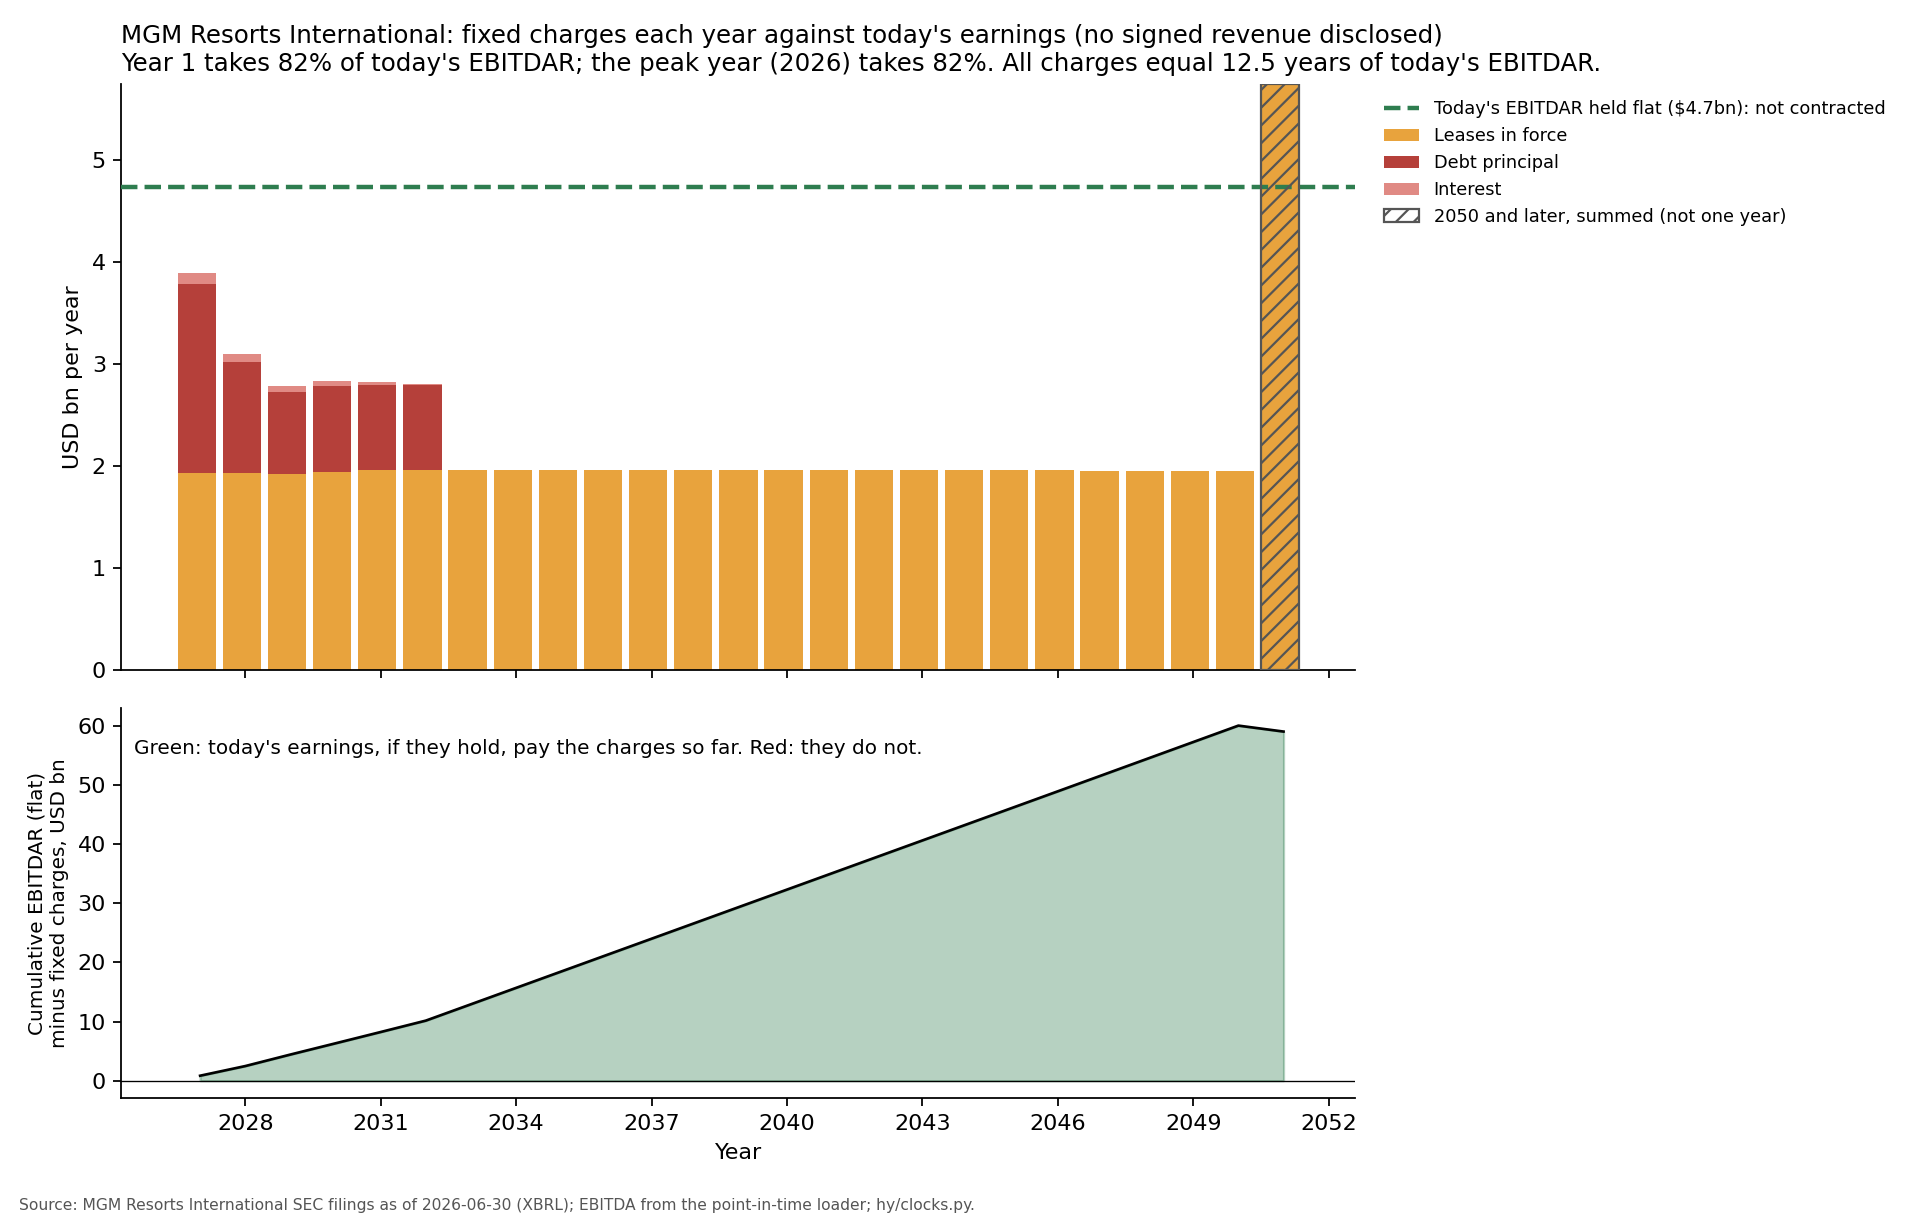
\includegraphics[width=0.95\linewidth]{figures/clocks_all_MGM.png}\caption*{The two clocks (section G2.1).}\end{figure}
\begin{figure}[H]\centering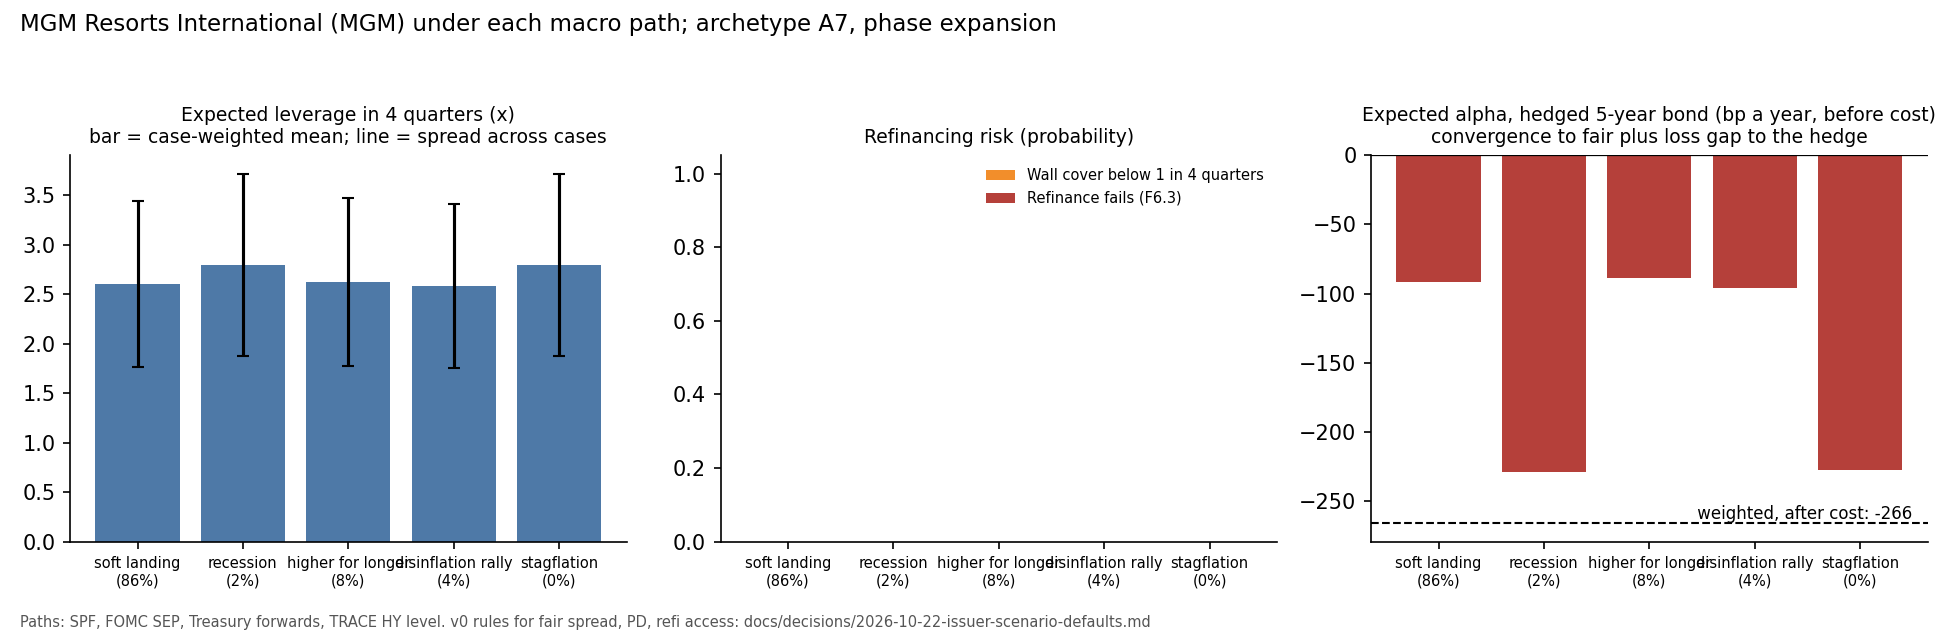
\includegraphics[width=0.95\linewidth]{figures/scenarios_MGM.png}\caption*{The company under each economic story (section G2.2).}\end{figure}
\begin{figure}[H]\centering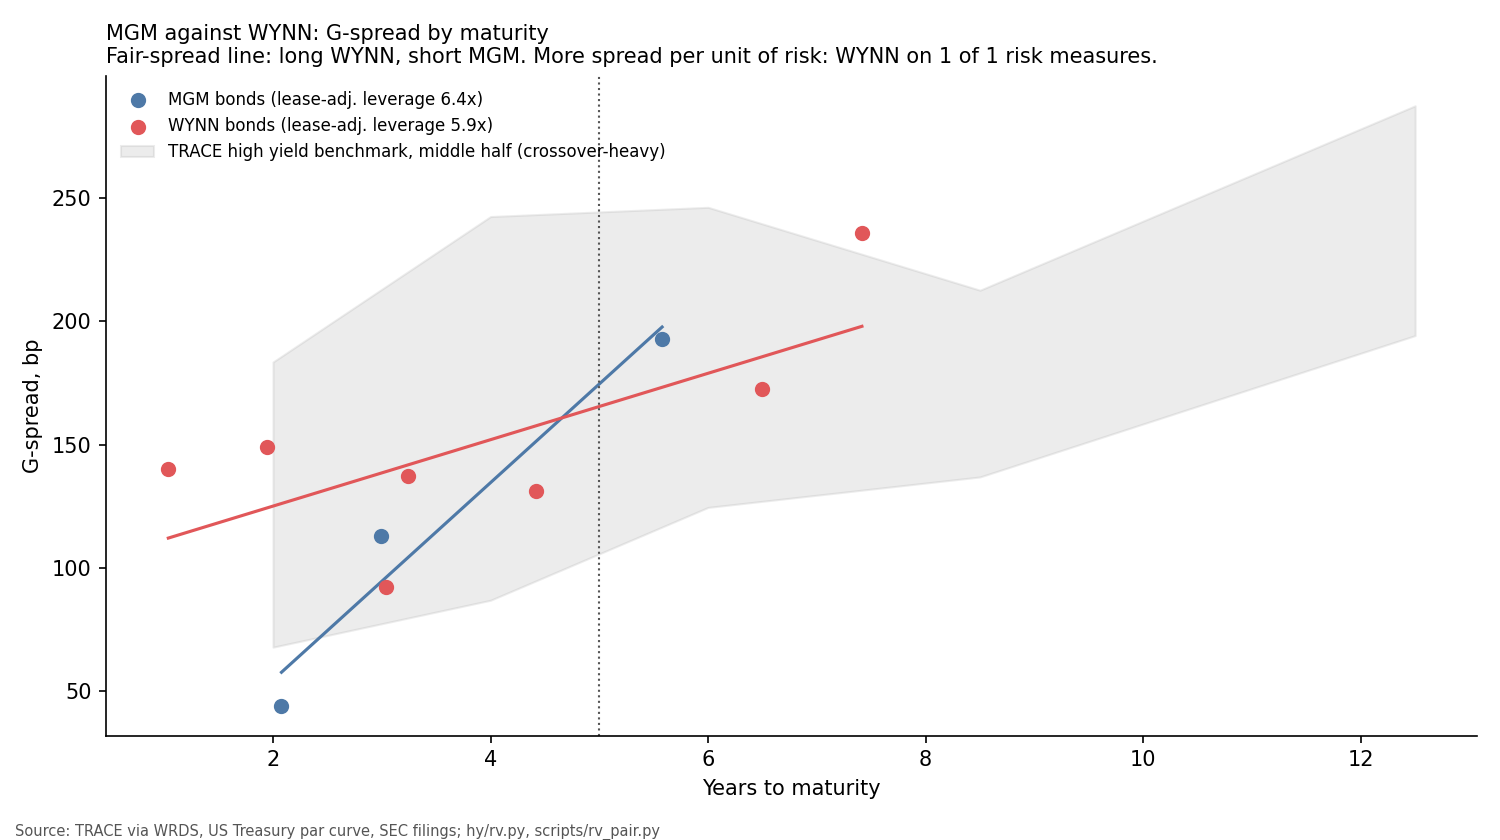
\includegraphics[width=0.85\linewidth]{figures/rv_MGM_WYNN.png}\caption*{The pair (section G2.3).}\end{figure}
\newpage
\section*{Wynn Resorts (WYNN)}\pdfbookmark[1]{WYNN}{bm-WYNN}\label{memo-start-WYNN}
\par\noindent\fcolorbox{gray}{gray!6}{\parbox{\dimexpr\linewidth-2\fboxsep-2\fboxrule-1pt}{\sloppy \textbf{Recommendation.} Pass. This is a view of the company, not a trade: the expected profit does not beat trading costs; the checks point in different directions. If the money went elsewhere, the best alternative in this run is NCLH. Position size and hedge: open until the call passes.}}

\subsection*{The combined view: four groups, one estimate}
Each group of methods estimates the same thing: what the bond should earn above a hedge, in bp a year. The combined estimate weighs the four groups. It ranks 7 of the issuers in this run. 3 of 5 groups point the same way as the combination.
\begin{center}\footnotesize\setlength{\tabcolsep}{3.5pt}\begin{tabular}{@{}lrrrl@{}}\toprule
Group & bp a year & Weight & Adds & Call \\\midrule
G1. Core process & -22 & 45\% & -10 & \textcolor{bad}{against owning} \\
G2 clocks. Two clocks & +4 & 20\% & +1 & \textcolor{amber}{leans to owning} \\
G2 rest. Built methods (rest) & -58 & 12\% & -7 & \textcolor{bad}{against owning} \\
G3. Credit skills & +0 & 12\% & +0 & \textcolor{good}{no objection} \\
G4. Books & -148 & 12\% & -17 & \textcolor{bad}{against owning} \\
\textbf{Combined, before trading costs} &  &  & \textbf{-33} &  \\
Trading costs &  &  & -172 &  \\
\textbf{Combined, after trading costs} &  &  & \textbf{-205} &  \\
Weighted cases and stories alone, after costs &  &  & -336 &  \\
Calibrated: after-cost number x measured slope 0.079 &  &  & -16 &  \\
\bottomrule\end{tabular}\end{center}
Against the weighted cases and stories alone, the combination is 131 bp a year higher: the other methods add to the case for owning the bond. A group that supports owning must beat the trading costs on its own. The weights are the user's choice: core process 45\%, two clocks 20\%, and 11.7\% each for the rest of the built methods, the credit skills and the books. The backtest alone would have put most weight on the built methods.
\par\noindent\fcolorbox{gray}{gray!6}{\parbox{\dimexpr\linewidth-2\fboxsep-2\fboxrule-1pt}{\sloppy \textbf{Alpha sizes are uncalibrated.} The backtest (2008 to 2026) shows that this kind of estimate ranks bonds well but overstates the size of the move. Realised alpha has been about 0.08 times the predicted alpha (standard error 0.05; 0.25 since 2019). The calibrated number multiplies by that slope: -16 bp a year after costs (-52 on the 2019 slope). The slope is not above zero by two standard errors, so the number ranks the bond but does not size it. Decision page: 2026-10-22-alpha-backtest-design. The backtest has no default-loss term yet.}}

\section*{G1. Core process: Gatto's steps, our method and rulebook, the relative value paper}
\par\noindent\fcolorbox{gray}{gray!6}{\parbox{\dimexpr\linewidth-2\fboxsep-2\fboxrule-1pt}{\sloppy \textbf{Verdict: \textcolor{bad}{against owning}.} This group reads Gatto's seven steps, our method and rulebook, and the relative value paper. Its estimate of expected profit is -22 bp a year before trading costs (costs are 172 bp a year); 2 of 4 of its weighted estimates point the same way. It carries 45\% of the combined view and ranks 7 of the issuers on this group alone. Best alternative for the same money: NCLH.}}
\begin{center}\footnotesize\setlength{\tabcolsep}{3.5pt}\begin{tabular}{@{}p{6.2cm}rrrp{4.2cm}@{}}\toprule
Estimate & bp a year & Weight in group & Adds & Where it comes from \\\midrule
Default chance the price assumes (shown, weight 0) & -20 & 0\% & -0 & F9; mapping C2 \\
Earnings quality, add-backs, FCF check (can only lower) & +0 & 25\% & +0 & F3; ebitda-addback-treatment; hy-model-standards \\
Access to new money and the funding gap & +96 & 25\% & +24 & F4; RV PDF E75-E76 \\
Debt against market value & -178 & 25\% & -44 & F7.7 \\
Return above cash, repriced in every story & -6 & 25\% & -2 & RV PDF E50-E60; C1, C3 \\
\bottomrule\end{tabular}\end{center}
\subsection*{G1.1 Thesis}
The bond pays 165 bp over Treasuries at 5 years. A company with its leverage (6.0x with leases) pays 226 bp on the fair line, so the bond is expensive by 60 bp. What would reveal it, and when: open question.
\subsection*{G1.2 The business}
\begin{enumerate}
\item \textbf{What it sells:} Wynn Resorts, Limited ("Wynn Resorts," "Wynn," or together with its subsidiaries, "we" or the "Company") is a preeminent designer, developer, and operator of integrated resorts featuring luxury hotel rooms, high-end retail space, an array of dining and entertainment options, meeting and convention facilities, and gaming, all supported by an unparalleled focus on our guests, our people, and our community. We believe that our extensive design and operational experience across numerous gaming juris
\item \textbf{How it earns:} revenue 7.4bn a year at a 24\% EBITDA margin.
\item \textbf{What it must spend to stand still:} rent of about \$0.0bn a year, plus maintenance capital spending.
\item \textbf{Competition:} open question.
\item \textbf{What breaks it:} an asset-specific shock or a block on distributions.
\end{enumerate}
Business type: A7.
\subsection*{G1.3 Earnings, normalised}
Last 12 months: EBITDA \$1.8bn at a 24\% margin; margin trend over 8 quarters -1.6 (t-statistic: above 1 rising, below $-1$ falling). One-off items \$-0.0bn. Free cash flow \$0.8bn: 44\% of EBITDA. Earnings-quality flags raised: EQ5 recurrence, FCF check (waterfall against OCF less capex) (of 5 tests the data supports). The add-back detail is in section G3.1.
\subsection*{G1.4 Cash, the funding gap, and the refinancing shock}
\begin{center}\footnotesize\setlength{\tabcolsep}{3.5pt}\begin{tabular}{@{}lr@{}}\toprule
Item & Value \\\midrule
Cash & \$2.1bn \\
Unused credit lines (tagged) & \$0.0bn \\
Less cash needed to run & \$0.0bn \\
Liquidity & \$2.1bn \\
Runway at today's cash burn, all capital spending (quarters) & no burn \\
First quarter cash runs out, severe case, maintenance spending only & no shortfall in 8 quarters \\
First quarter cash runs out, severe case, all committed spending & no shortfall in 8 quarters \\
\textbf{Runway we quote (the shortest)} & \textbf{none in 8 quarters} \\
Debt due in the next 18 months & \$0.0bn \\
Cash to meet debt due in a year, base case & 347.38x \\
Refinancing access score, likely story (0 to 6) & 3 \\
\bottomrule\end{tabular}\end{center}
\textbf{Funding gap if no lender refinances.} We add cash, the unused lines and the free cash flow of the cases, then take off the debt as it falls due, quarter by quarter. The minimum cash kept back is one month of cash operating costs (\$0.5bn).
\begin{center}\footnotesize\setlength{\tabcolsep}{3.5pt}\begin{tabular}{@{}lr@{}}\toprule
Measure & Value \\\midrule
Lowest point, likely story (maintenance spending only) & \$1.2bn \\
First quarter below zero, likely story & none in 8 quarters \\
Lowest point with all capital spending & \$1.2bn \\
First quarter below zero with all capital spending & none in 8 quarters \\
Lowest point, severe case & \$0.2bn \\
Severe case with all capital spending: first quarter below zero & no gap in 8 quarters \\
Lowest point, weighted over the stories & \$1.2bn \\
Debt due inside 8 quarters, share of all debt & 27\% \\
\bottomrule\end{tabular}\end{center}
\textbf{Refinancing shock.} \$2.9bn falls due in the next two years. It pays about 5.56\% today (TRACE coupons of bonds due inside 27 months). Refinanced at the forecast Treasury rate plus today's spread, yearly interest changes by \$0.0bn (1.8\% of EBITDA). Interest cover after refinancing: 2.7x; after capital spending 1.7x. Free cash flow after the shock: 7.1\% of debt.
\subsection*{G1.5 Debt: going-concern view}
\begin{center}\footnotesize\setlength{\tabcolsep}{3.5pt}\begin{tabular}{@{}lr@{}}\toprule
Measure & Value \\\midrule
Debt & \$10.7bn \\
Lease liabilities & \$0.0bn \\
EBITDA, last 12 months & \$1.8bn \\
Debt / EBITDA & 6.0x \\
(Debt + leases) / (EBITDA + rent) & 6.0x \\
Net debt / EBITDA & 5.1x \\
Coverage (after all capital spending) & 1.8x \\
Fixed-charge cover (after maintenance spending) & 1.86x \\
\bottomrule\end{tabular}\end{center}
\begin{center}\footnotesize\setlength{\tabcolsep}{3.5pt}\begin{tabular}{@{}lrrrrr@{}}\toprule
Bond & Coupon & Matures & Price & Yield & Spread (bp) \\\midrule
98313RAD8 & 5.50\% & 2027-10-01 & 99.7 & 5.81\% & 140 \\
98313RAH9 & 5.63\% & 2028-08-26 & 99.1 & 6.14\% & 149 \\
983133AA7 & 5.12\% & 2029-10-01 & 98.5 & 5.67\% & 92 \\
98313RAE6 & 5.12\% & 2029-12-15 & 97.1 & 6.13\% & 137 \\
983133AC3 & 7.12\% & 2031-02-15 & 103.8 & 6.08\% & 131 \\
983133AD1 & 6.25\% & 2033-03-15 & 98.3 & 6.57\% & 173 \\
\bottomrule\end{tabular}\end{center}
Claims view (who is paid what in a default): open question until the debt documents are read.
\subsection*{G1.6 Company value}
Market value of the whole company \$19bn (shares \$10bn plus net debt): 10.6x EBITDA; debt is 56\% of it. Our own valuation range and the bonds' recovery if the company defaults: open questions (they need a peer set and a distressed multiple).
\subsection*{G1.7 The decision against cash}
We put the same money in the bond nearest five years (983133AC3, 7.12\% due 2031-02-15, price 103.79 plus 0.62 accrued) or in six-month Treasury bills at 4.20\%. In each story the bond either survives and is repriced, or defaults and returns 35 per 100 (a 40\% recovery paid a year later, valued at 15\% a year). In default the holder loses 67\% of the price paid.
\begin{center}\footnotesize\setlength{\tabcolsep}{3.5pt}\begin{tabular}{@{}lr@{}}\toprule
Measure & Value \\\midrule
Expected return above cash, bp a year & -6 \\
Chance of a loss over six months & 9.4\% \\
Chance of doing worse than cash & 9.4\% \\
Average loss in the worst 5\% of outcomes & 12.1\% \\
Same, with rates and the market hedged out, bp a year & -142 \\
Best alternative in this run (worst 5\% loss within the 25\% budget) & NCLH \\
Return given up against that alternative, bp a year & +452 \\
\bottomrule\end{tabular}\end{center}
\section*{G2. Built methods: two clocks, stories and cases, relative value, the gate}
\par\noindent\fcolorbox{gray}{gray!6}{\parbox{\dimexpr\linewidth-2\fboxsep-2\fboxrule-1pt}{\sloppy \textbf{Verdict: \textcolor{bad}{against owning}.} This group reads the spread level, the fair line and the pair, the economic stories, the health panel. Its estimate of expected profit is -58 bp a year before trading costs (costs are 172 bp a year); 4 of 5 of its weighted estimates point the same way. It carries 12\% of the combined view and ranks 5 of the issuers on this group alone. Gate: pass.}}
\begin{center}\footnotesize\setlength{\tabcolsep}{3.5pt}\begin{tabular}{@{}p{6.2cm}rrrp{4.2cm}@{}}\toprule
Estimate & bp a year & Weight in group & Adds & Where it comes from \\\midrule
Spread level: the extra pay over the market (carry) & -2 & 42\% & -1 & Spec S14 E0; K15 \\
Weighted cases and stories & -164 & 25\% & -41 & M5.4, M7.5 \\
Spread against the fair line & -144 & 17\% & -24 & M7.4, M7.5 \\
The pair & +109 & 8\% & +9 & M7.4; F10 S4 \\
Health panel & -6 & 8\% & -1 & F8 \\
\bottomrule\end{tabular}\end{center}
\subsection*{G2.1 The two clocks: bills against what pays for them}
\par\noindent\fcolorbox{gray}{gray!6}{\parbox{\dimexpr\linewidth-2\fboxsep-2\fboxrule-1pt}{\sloppy \textbf{Verdict: \textcolor{amber}{leans to owning}.} This group reads the bills the company owes against the revenue customers have signed for. Its estimate of expected profit is +4 bp a year before trading costs (costs are 172 bp a year); 1 of 1 of its weighted estimates point the same way. It carries 20\% of the combined view and ranks 5 of the issuers on this group alone. The clocks count as their own bucket in the combined view.}}
\begin{center}\footnotesize\setlength{\tabcolsep}{3.5pt}\begin{tabular}{@{}p{6.2cm}rrrp{4.2cm}@{}}\toprule
Estimate & bp a year & Weight in group & Adds & Where it comes from \\\midrule
The two clocks & +4 & 100\% & +4 & M4.7 \\
\bottomrule\end{tabular}\end{center}
Fixed bills total \$16.7bn, centred 5.9 years out: leases in force \$4.3bn, debt principal \$10.6bn, interest \$1.8bn. That is 9.3 years of today's EBITDAR; next year's bills take 115\% of it.
The company discloses no material signed revenue, so the second clock is today's earnings held flat (chart at the end).
\subsection*{G2.2 Economic stories and cases}
Cases on the most likely story (soft landing), stage of the cycle: expansion.
\begin{center}\scriptsize\setlength{\tabcolsep}{3.5pt}\begin{tabular}{@{}lrrrrrrr@{}}\toprule
Case & Weight & Growth / qtr & Leverage in 1 yr & Peak leverage & Lowest liquidity & Cash runs out & Refi fails \\\midrule
base & 60\% & 1.6\% & 5.6x & 5.9x & \$2.4bn & no & no \\
down moderate & 15\% & 1.9\% & 6.7x & 6.7x & \$2.3bn & no & no \\
down severe & 5\% & 1.9\% & 9.3x & 9.3x & \$2.2bn & no & no \\
upside & 20\% & 1.8\% & 4.8x & 5.5x & \$2.4bn & no & no \\
\bottomrule\end{tabular}\end{center}
\begin{center}\scriptsize\setlength{\tabcolsep}{3.5pt}\begin{tabular}{@{}lrrrrrr@{}}\toprule
Story & Chance & Leverage in 1 yr & Peak leverage (down) & Refi fails & Default chance & Expected profit (bp/yr) \\\midrule
soft landing & 86\% & 5.8x & 9.3x & 0\% & 1.6\% & -158 \\
recession & 2\% & 6.2x & 10.0x & 0\% & 4.1\% & -409 \\
higher for longer & 8\% & 5.8x & 9.4x & 0\% & 1.9\% & -187 \\
disinflation rally & 4\% & 5.7x & 9.2x & 0\% & 1.2\% & -123 \\
stagflation & 0\% & 6.2x & 10.0x & 0\% & 4.1\% & -416 \\
\bottomrule\end{tabular}\end{center}
\subsection*{G2.3 Relative value and the pair}
Fair line: log spread = -5.64 + 0.312 x leverage, fitted on 8 issuers in this run. 5-year spread 165 bp against a fair 226 bp.
\textbf{Against peers.} Peers are the high yield bonds that traded in 2026-08-31 (733 bonds with leverage on file), in the same 3 to 7 year maturity bucket. Sector: Consumer Discretionary. Rating class: B (implied by leverage). A positive value means the issuer pays more than the median peer.
\begin{center}\footnotesize\setlength{\tabcolsep}{3.5pt}\begin{tabular}{@{}lrr@{}}\toprule
Peer group & Excess spread to peers (ESP) & Spread per turn against peers (E13) \\\midrule
Sector and rating & -34\% & -35\% \\
Sector only & -1\% & -13\% \\
Rating only & -3\% & -14\% \\
\bottomrule\end{tabular}\end{center}
\textbf{SPiDER} (spread per unit of debt to 10-year average EBITDA; Dynkin et al. 2021, ch. 14): cheaper than 24\% of the peer bonds across all sectors, and -65\% against sector and rating peers. It has no weight in the score: its edge beyond spread level is small (t 1.3 at 12 months).
\textbf{Against MGM.} Spreads at 5 years: MGM 175 bp, WYNN 165 bp.
\begin{center}\footnotesize\setlength{\tabcolsep}{3.5pt}\begin{tabular}{@{}lrrr@{}}\toprule
Spread per & MGM & WYNN & Cheaper \\\midrule
turn of leverage & 27 & 28 & WYNN \\
\bottomrule\end{tabular}\end{center}
The fair line favours long WYNN, short MGM: a gap of 13 bp, which halves in about 2 weeks on six months of trades. Under the stories the pair earns soft landing +56, recession +146, higher for longer +67, disinflation rally +63, stagflation +149 bp a year; weighted +59 bp before costs.
\subsection*{G2.4 Expected profit and price against our view}
Hedged 5-year bond over six months: -164 bp a year before trading costs, -336 bp after. It does not beat costs. The expected default loss is charged on the price paid: 67\% of it in default, not 60\% of face.
\begin{center}\footnotesize\setlength{\tabcolsep}{3.5pt}\begin{tabular}{@{}p{5.2cm}rrrrl@{}}\toprule
Question & Price assumes & Our view & Gap & Noise & Gap bigger than noise? \\\midrule
Default chance at the v0 price of risk (shown, not tested) & 1.4\% & 1.6\% & 0.3\% & open & not tested \\
Breakeven default probability, 12 months (loss on price) & 2.5\% & 1.6\% & -0.8\% & 1.2\% & no \\
Leverage the spread is pricing & 4.95 & 5.95 & 1.00 & 0.90 & yes \\
Spread against fair (bp) & 165 & 226 & 60 & 63 & no \\
Rating class & open & BB & open & open & not tested \\
Recovery if default (per 1 of face, discounted for delay) & open & 0.35 & open & open & not tested \\
\bottomrule\end{tabular}\end{center}
The first row turns the spread into a default chance with a fixed price of risk. That is not a real default chance, so it is shown but not tested. The breakeven row asks a cleaner question: is our default chance below the rate at which the spread only just pays for default losses?
\subsection*{G2.5 Risks and the health panel}
\begin{itemize}\item Margins are falling. Tracked by: margin trend (t-statistic) (-1.61). Resolves when: two quarters of stable margins.\end{itemize}
\begin{center}\footnotesize\setlength{\tabcolsep}{3.5pt}\begin{tabular}{@{}lrl@{}}\toprule
Measure & Value & Band \\\midrule
Margin trend (t-statistic) & -1.61 & \textcolor{bad}{red} \\
Coverage & 1.80 & \textcolor{amber}{amber} \\
Free cash flow / debt & 0.07 & \textcolor{amber}{amber} \\
Refinancing access score (0 to 6) & 3.00 & \textcolor{amber}{amber} \\
Earnings-quality flags & 2.00 & \textcolor{amber}{amber} \\
Fixed-charge cover & 1.86 & \textcolor{good}{green} \\
Cash conversion (FCF / EBITDA) & 0.44 & \textcolor{good}{green} \\
Cash to meet debt due in 1 year (base case) & 347.38 & \textcolor{good}{green} \\
Weight on the downside cases & 0.20 & \textcolor{good}{green} \\
Chance debt due in 1 year is not covered & 0.00 & \textcolor{good}{green} \\
Chance cash runs out within 2 years & 0.00 & \textcolor{good}{green} \\
\bottomrule\end{tabular}\end{center}
\section*{G3. Credit skills: the lender's checklists applied to a public bond}
\par\noindent\fcolorbox{gray}{gray!6}{\parbox{\dimexpr\linewidth-2\fboxsep-2\fboxrule-1pt}{\sloppy \textbf{Verdict: \textcolor{good}{no objection}.} This group reads the lender's checklists: add-backs, covenants, watchlist, trend, memo structure. Its estimate of expected profit is +0 bp a year before trading costs (costs are 172 bp a year); 1 of 1 of its weighted estimates point the same way. It carries 12\% of the combined view and ranks 1 of the issuers on this group alone. Its estimates can only lower the combined number: a clean checklist earns no credit. Watchlist: none.}}
\begin{center}\footnotesize\setlength{\tabcolsep}{3.5pt}\begin{tabular}{@{}p{6.2cm}rrrp{4.2cm}@{}}\toprule
Estimate & bp a year & Weight in group & Adds & Where it comes from \\\midrule
Watchlist tier (can only lower) & +0 & 100\% & +0 & borrower-monitoring; covenant-compliance \\
\bottomrule\end{tabular}\end{center}
\subsection*{G3.1 Add-backs and their cash effect}
Reported EBITDA over the last 12 months is \$1.8bn. The company's own measure adds back \$0.0bn of one-off items to reach \$1.8bn: 0.0\% of reported EBITDA (a negative figure is a one-off gain taken out). This is under the 5\% line for one item. They do not recur in three quarters running. If every add-back were paid in cash, free cash flow would be \$0.8bn. The two roads to free cash flow (the EBITDA bridge, \$0.4bn; operating cash flow less capital spending, \$0.8bn) differ by 21\% of EBITDA: above the 10\% tolerance, so an earnings-quality flag is raised. The add-back table by category is an open question: the data has one total line.
\subsection*{G3.2 Covenant headroom}
The filing states these maintenance tests. We test them on our own ratio, which uses our EBITDA, not the covenant's, and the whole group.
\begin{center}\footnotesize\setlength{\tabcolsep}{3.5pt}\begin{tabular}{@{}p{3.8cm}rrrp{1.9cm}p{4.4cm}@{}}\toprule
Test & Level & Our ratio & Headroom & Band & Notes \\\midrule
a Consolidated First Lien Net Leverage Ratio & 3.75 & 4.78 & -28\% & proxy only (open) & binds a subsidiary group; our ratio is only a bound for this test; net debt / EBITDA \\
\bottomrule\end{tabular}\end{center}
No test can be read on our own ratio: each one binds a narrower group of debt or needs the credit lines. Headroom stays an open question; it does not move the watchlist.
\subsection*{G3.3 Watchlist and trajectory}
Watchlist tier: \textbf{none}: no trigger is met. EBITDA against the same months a year earlier: 0.8\% (no plan is public, so last year stands in for it).
\begin{center}\footnotesize\setlength{\tabcolsep}{3.5pt}\begin{tabular}{@{}llll@{}}\toprule
Measure & Direction & How much weight & Change on a year earlier, last quarter \\\midrule
revenue & improving & trend & 6.9\% \\
EBITDA & improving & data point & 10.9\% \\
EBITDA margin & improving & observation & 3.8\% \\
cash conversion & improving & trend & 27.4\% \\
\bottomrule\end{tabular}\end{center}
One quarter is an observation, two a data point, three or four a trend.
\subsection*{G3.4 Memo structure check}
\begin{center}\footnotesize\setlength{\tabcolsep}{3.5pt}\begin{tabular}{@{}lp{9cm}l@{}}\toprule
Section & Requires & Status \\\midrule
Executive summary & the business in one sentence, the opportunity, 2 to 3 reasons, 2 to 3 risks & \textcolor{good}{pass} \\
Capital structure & each tranche with face, coupon, maturity; senior, total and net leverage; LTV & \textcolor{amber}{open} \\
Terms & maintenance covenant levels and test dates; incurrence baskets; call terms & \textcolor{amber}{open} \\
Investment merits & free cash flow generation and the base-case deleveraging path & \textcolor{good}{pass} \\
Key risks & 3 to 5 issuer-specific risks, each with a mitigant & \textcolor{good}{pass} \\
Historical financials & at least 3 years, quarterly where available & \textcolor{good}{pass} \\
EBITDA adjustments & reported-to-adjusted bridge with the load as a share of EBITDA and the 5\% flag & \textcolor{amber}{open} \\
Model output & base and downside: EBITDA, FCF, leverage path, covenant headroom, liquidity runway & \textcolor{amber}{open} \\
\bottomrule\end{tabular}\end{center}
\textbf{Rules that do not transfer to a public bond:}\begin{itemize}\item The compliance certificate is the source of truth; public bonds have none. Headroom here uses our own ratio against a level parsed from the filing text. (covenant-compliance)\item Equity cures, step-down schedules and window-dressing checks need the credit agreement and monthly revolver balances. (covenant-compliance)\item Performance against the sponsor plan: no plan is public. The proxy is the same quarters a year earlier. (borrower-monitoring)\item Add-back caps and the certificate reconciliation live in the credit agreement. Compustat gives one special-items line, not the category table. (ebitda-addback-treatment)\item Sources and uses at entry, the sponsor case and the management call apply to new loans, not to bonds bought in the secondary market. (credit-memo-standards)\item Monthly lender packages do not exist for public issuers; XBRL quarters replace them. (quarterly-package-extraction)\end{itemize}
\section*{G4. Books: Kricheff, and Ganguin and Bilardello (S\&P)}
\par\noindent\fcolorbox{gray}{gray!6}{\parbox{\dimexpr\linewidth-2\fboxsep-2\fboxrule-1pt}{\sloppy \textbf{Verdict: \textcolor{bad}{against owning}.} This group reads Kricheff's cash bridge and ratios; the S\&P risk profiles and rating anchor. Its estimate of expected profit is -148 bp a year before trading costs (costs are 172 bp a year); 2 of 2 of its weighted estimates point the same way. It carries 12\% of the combined view and ranks 8 of the issuers on this group alone. S\&P anchor class: BB.}}
\begin{center}\footnotesize\setlength{\tabcolsep}{3.5pt}\begin{tabular}{@{}p{6.2cm}rrrp{4.2cm}@{}}\toprule
Estimate & bp a year & Weight in group & Adds & Where it comes from \\\midrule
Spread against the S\&P risk score & -190 & 50\% & -95 & Ganguin and Bilardello ch. 10 \\
Spread per turn of leverage (with the trap guard) & -106 & 50\% & -53 & Kricheff ch. 21 \\
\bottomrule\end{tabular}\end{center}
\subsection*{G4.1 Kricheff's cash-flow bridge and ratio set}
\begin{center}\footnotesize\setlength{\tabcolsep}{3.5pt}\begin{tabular}{@{}lr@{}}\toprule
Line (last 12 months) & Value \\\midrule
Adjusted EBITDA & \$1.8bn \\
less capital spending & \$0.7bn \\
less cash interest & \$0.6bn \\
less cash taxes & \$0.1bn \\
less increase in working capital & \$-0.0bn \\
\textbf{Free cash flow} & \textbf{\$0.4bn} \\
Check: free cash flow before capital spending less operating cash flow & \$-0.4bn \\
Free cash flow after dividends & open (dividends not loaded) \\
\bottomrule\end{tabular}\end{center}
\begin{center}\footnotesize\setlength{\tabcolsep}{3.5pt}\begin{tabular}{@{}lrlr@{}}\toprule
Ratio & Value & Ratio & Value \\\midrule
EBITDA / cash interest & 2.9x & Debt / EBITDA & 6.0x \\
(EBITDA $-$ capex) / interest & 1.8x & Net debt / EBITDA & 4.8x \\
(EBITDA $-$ maintenance capex) / interest & 1.9x & Free cash flow / debt & 7.0\% \\
EBITDA / debt (highest rate at 1x cover) & 17.0\% & Market value / EBITDA & 10.3x \\
Equity cushion (1 $-$ debt / market value) & 43\% & Spread per turn of leverage & 28 bp \\
\bottomrule\end{tabular}\end{center}
Kricheff's snapshot rule: operating cash flow covers capital spending. Spread per turn compares the bond with the run's median of 38 bp a turn. Kricheff warns that a high spread per turn can mean weak cash flow, not value; read it with free cash flow / debt. The book measures leverage through each bond's rank; with no face by rank, total leverage stands in.
\subsection*{G4.2 The S\&P risk profiles and the rating anchor}
S\&P adds leases to debt and scores each ratio against the median of each rating class (CreditStats 2002, from the book). Scores run from 1 (safest) to 10 (default).
\begin{center}\footnotesize\setlength{\tabcolsep}{3.5pt}\begin{tabular}{@{}lrrrr@{}}\toprule
Ratio & Value & Score & BB median & B median \\\midrule
Debt / (debt + market value of equity) & 52\% & 6.5 & 57.5\% & 78.5\% \\
Funds from operations / debt & 13\% & 8.9 & 19.5\% & 10.8\% \\
Free operating cash flow / debt & 7\% & 7.9 & 8.5\% & 2.5\% \\
EBITDA / interest (with lease interest) & 2.9x & 8.0 & 3.2x & 1.8x \\
EBITDA margin & 24\% & 3.0 &  &  \\
\bottomrule\end{tabular}\end{center}
Financial risk score 7.2. Business risk score 5.5: industry 6, steadiness of sales 5 (year-on-year growth varies by 5.8\%), customer spread 5. The book puts 45\% of the weight on business risk for this class, so the default risk score is 6.4: the \textbf{BB} class. The line from score to spread across the run did not slope upward, so it gives no estimate. The 2005 edition has no modern anchor table; its own weighting table stands in for it.
\section*{Coming events, open questions, and the record}
\begin{itemize}\item Next quarterly results (estimated from filing cadence): 2026-11-05 (estimate).\item Debt due by 1.0 years out:  - \$0.0bn.\end{itemize}
\textbf{Open questions, most important first:}\begin{enumerate}\item A dated catalyst that would close the gap (G2).\item The observable and level that would prove the call wrong (G8).\item Face amount of each tranche and the secured debt ahead of the bonds (debt note table).\item Claims view: allowed claims by class and the entity map (framework F5).\item Covenant 'a Consolidated First Lien Net Leverage Ratio': our ratio is only a bound for this test (subsidiary group, narrower debt, or untagged credit lines); read the credit agreement definition.\item Revolver commitment, draw, and borrowing base: not tagged; read the credit agreement note.\item F4 points 3 (unencumbered assets) and 6 (sponsor support) are scored 0 until read.\item Recovery, delay and the required return on a defaulted claim are v0 (R = 0.4, tau = 1 year, k = 15\%); the claims view and documents replace them.\item Peer set of at least four issuers of the same archetype (F3.3) for the valuation range (F7.1).\item Distressed multiple (F7.3) and the recovery of the bonds if the company defaults (F7.9).\end{enumerate}
\textbf{Record (filled at exit):} exit date; return against the rating-matched index; worst point against the index; reason; the rule that would have helped.
\newpage
\begin{figure}[H]\centering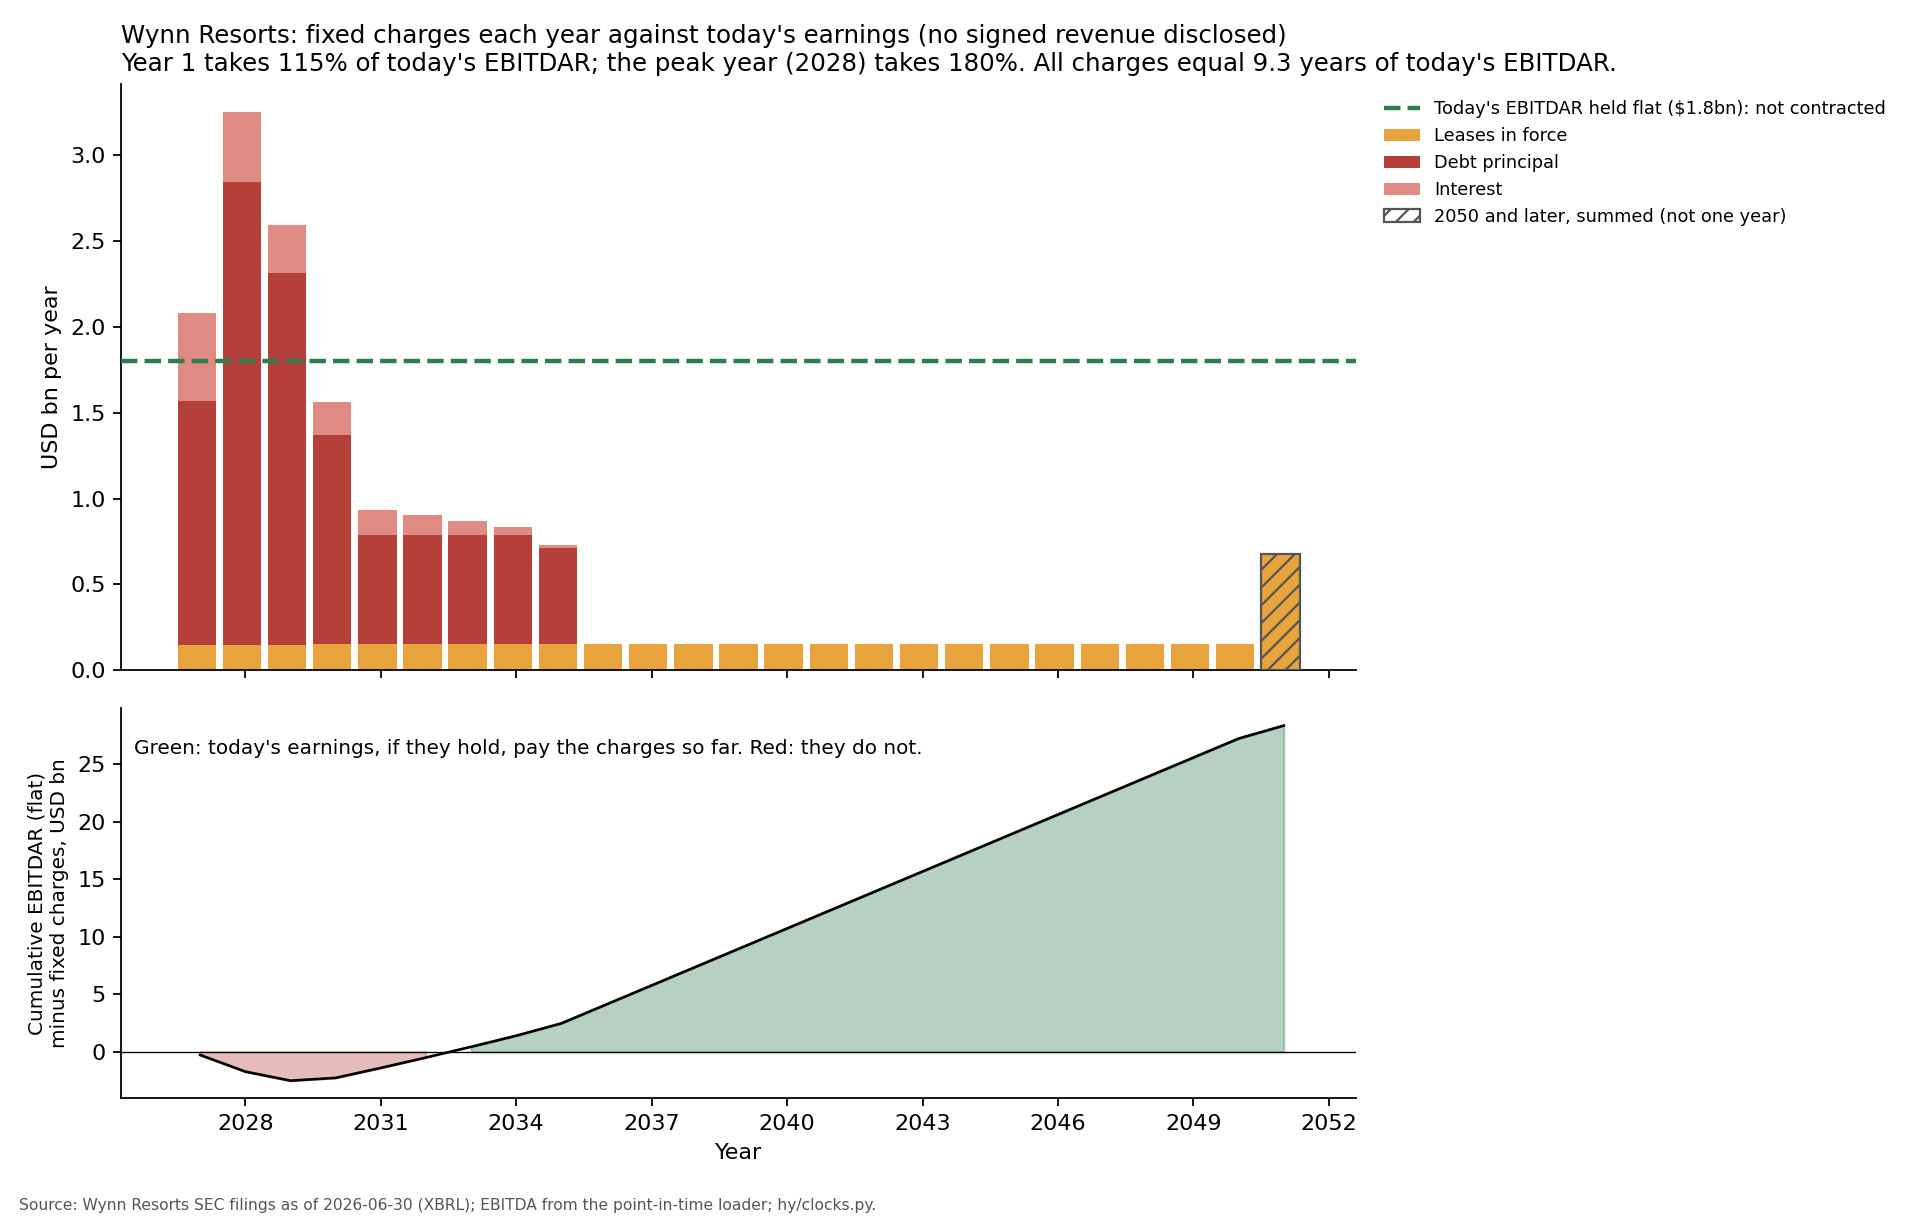
\includegraphics[width=0.95\linewidth]{figures/clocks_all_WYNN.png}\caption*{The two clocks (section G2.1).}\end{figure}
\begin{figure}[H]\centering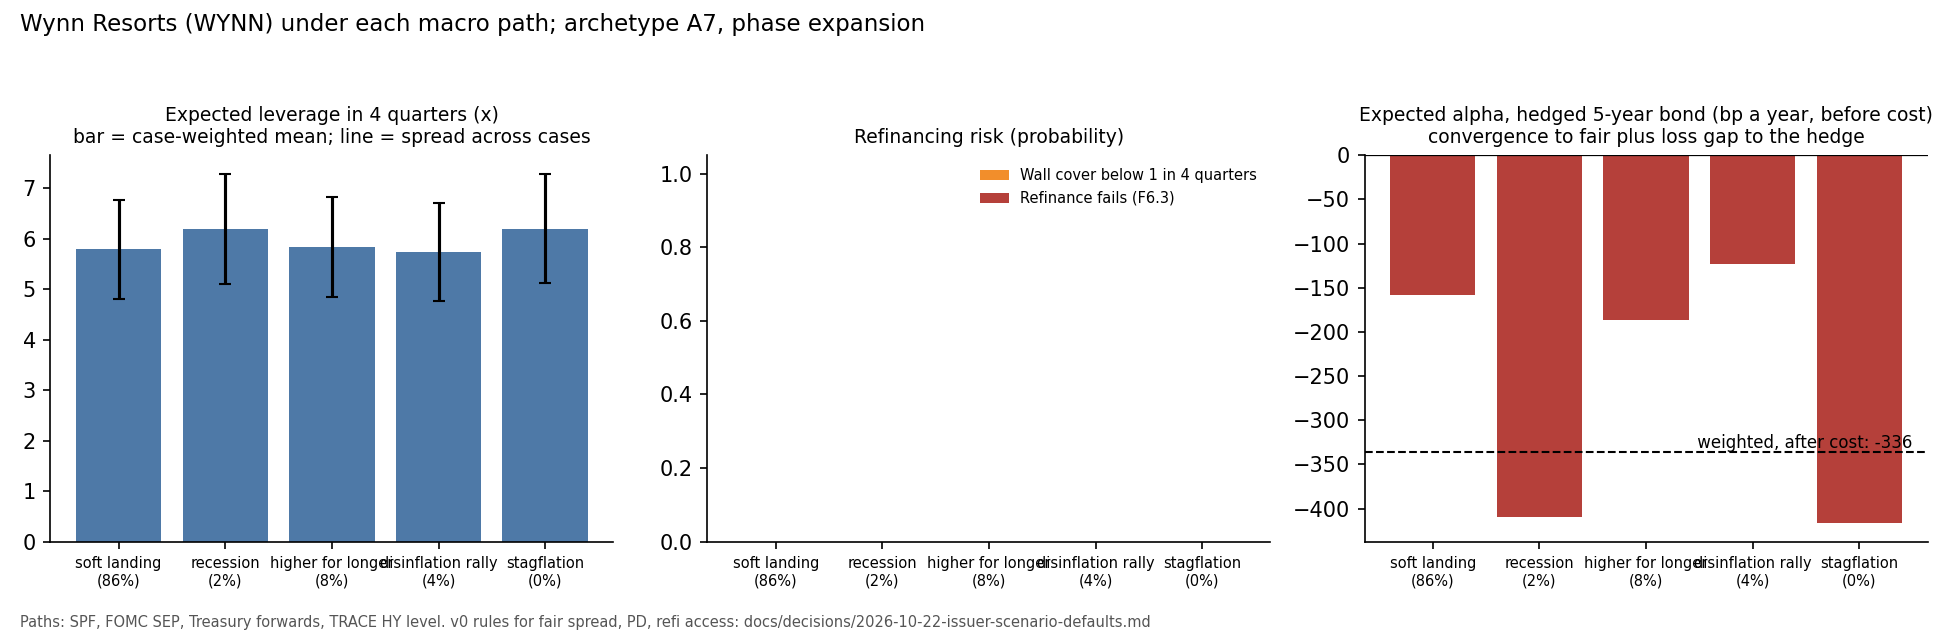
\includegraphics[width=0.95\linewidth]{figures/scenarios_WYNN.png}\caption*{The company under each economic story (section G2.2).}\end{figure}
\begin{figure}[H]\centering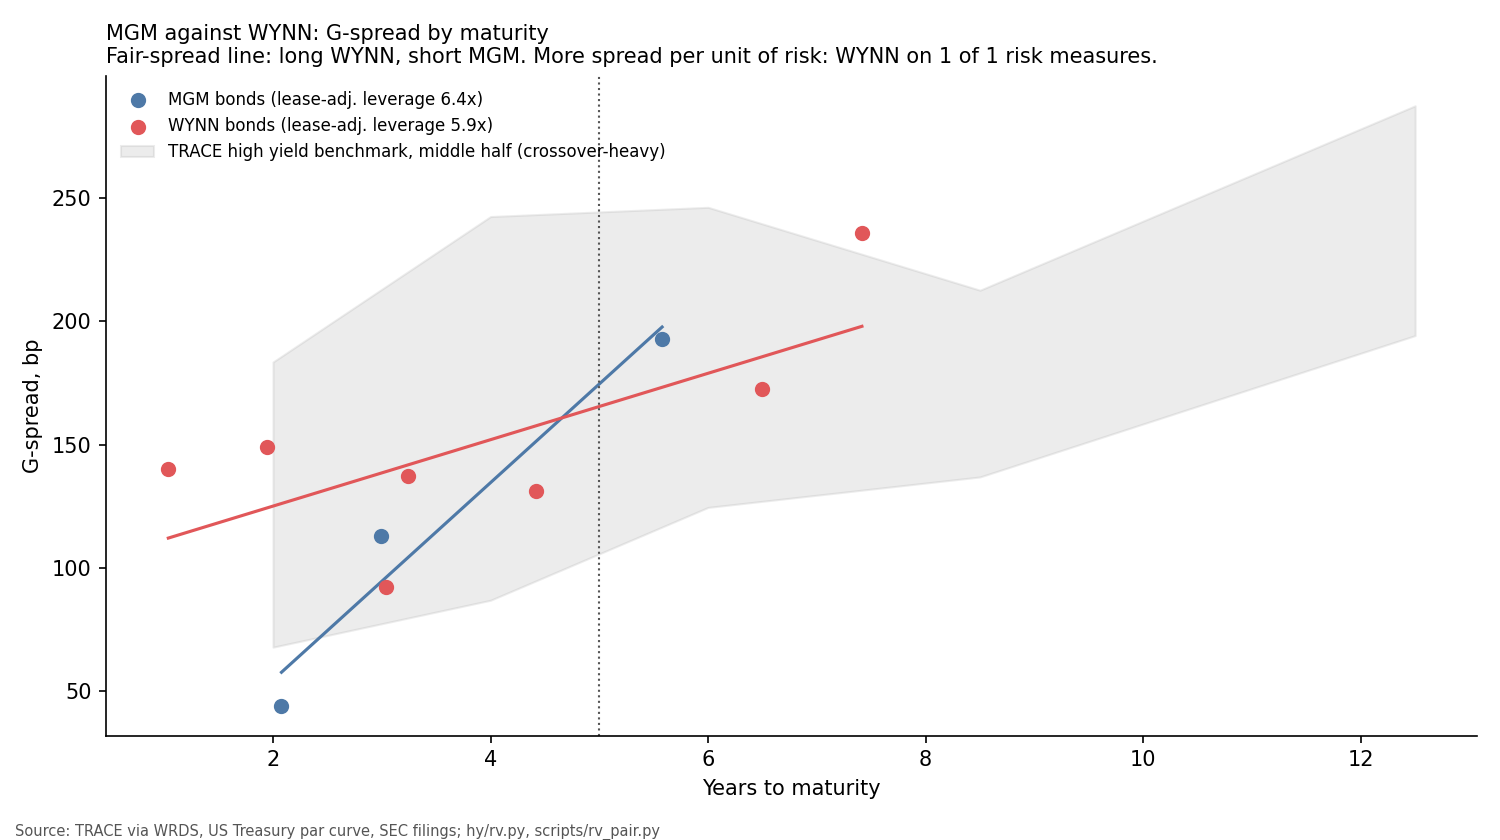
\includegraphics[width=0.85\linewidth]{figures/rv_MGM_WYNN.png}\caption*{The pair (section G2.3).}\end{figure}
\newpage
\end{document}
